\documentclass[specialist,
substylefile = spbu_report.rtx,
subf,12pt]{disser}

\usepackage[utf8]{inputenc}
\usepackage[T2A]{fontenc}
\usepackage[english,russian]{babel}
\usepackage{hyperref}
\hypersetup{unicode=true, pdfencoding=auto,
    colorlinks=true,
    linkcolor=blue,
    citecolor=blue,
    filecolor=blue,
    urlcolor=blue}

\usepackage[a4paper,
mag=1000, includefoot,
left=3cm, right=1.5cm, top=2cm, bottom=2cm, headsep=1cm, footskip=1cm]{geometry}

\usepackage{graphicx,subcaption,ragged2e}

\usepackage{caption}

\usepackage{booktabs}

\usepackage{amsthm}
\usepackage{amsmath}
\usepackage{amssymb}
\usepackage{mathtools}
\usepackage{hhline}
\usepackage{xcolor}
\usepackage{array}
\usepackage{bbm}
\usepackage{bm}

\usepackage{slashbox}

\usepackage{algorithm}
\usepackage{algorithmicx}

\floatname{algorithm}{Алгоритм}
\newcommand{\Input}{\emph{Входные данные: }}
\newcommand{\Output}{\emph{Результат: }}

\newcounter{algsubstate}
\renewcommand{\thealgsubstate}{\alph{algsubstate}}
\newenvironment{algsubstates}
  {\setcounter{algsubstate}{0}%
   \renewcommand{\State}{%
     \stepcounter{algsubstate}%
     \Statex {\footnotesize\thealgsubstate:}\space}}
  {}

\newcommand{\setlineformat}[1]{\algrenewcommand{\alglinenumber}[1]{#1}}

\theoremstyle{definition}
\newtheorem{definition}{Определение}[chapter]
\newtheorem{remark}{Замечание}[chapter]
\newtheorem{example}{Пример}[chapter]
\newtheorem{statement}{Утверждение}
\newtheorem{proposition}{Предложение}[chapter]
\newtheorem{corollary}{Следствие}[chapter]

\usepackage{cite}
\makeatletter
\newcommand{\citecomment}[2][]{\citen{#2}#1\citevar}
\newcommand{\citeone}[1]{\citecomment{#1}}
\newcommand{\citetwo}[2][]{\citecomment[,~#1]{#2}}
\newcommand{\citevar}{\@ifnextchar\bgroup{;~\citeone}{\@ifnextchar[{;~\citetwo}{]}}}
\newcommand{\citefirst}{\@ifnextchar\bgroup{\citeone}{\@ifnextchar[{\citetwo}{]}}}
\newcommand{\cites}{[\citefirst}
\makeatother

\newcommand{\R}{\mathbb{R}}
\newcommand{\const}{\mathrm{const}}
\newcommand{\im}{\mathrm{i}}

\usepackage{float}

\usepackage{rotating}

\input{letters_series_mathbb.tex}

\setcounter{tocdepth}{2}

\begin{document}

%
% Титульный лист на русском языке
%
% Название организации
\institution{%
	Санкт-Петербургский государственный университет\\
	Прикладная математика и информатика
}

\title{Учебная практика 2 (проектно-технологическая) (семестр 3)}

% Тема
\topic{Применение метода Monte Carlo SSA для анализа временных рядов}

% Автор
\author{Потешкин Егор Павлович}
\group{группа 24.M22-мм}

% Научный руководитель
\sa       {Голяндина Нина Эдуардовна \\%
	Кафедра Статистического Моделирования}
\sastatus {д.\,ф.-м.\,н., профессор}

% Город и год
\city{Санкт-Петербург}
\date{\number\year}

\maketitle

\tableofcontents

\intro
Метод Singular Spectrum Analysis (SSA)~\cite{Broomhead1986,Golyandina2001} является мощным инструментом для анализа временных рядов. Он позволяет разложить ряд на интерпретируемые компоненты, такие как тренд, периодические колебания и шум, что значительно упрощает процесс анализа. Метод Monte Carlo SSA~\cite{Allen1996}, в свою очередь, решает задачу обнаружения сигнала в шуме, проверяя соответствующую гипотезу.

Для наиболее распространенного варианта метода Monte Carlo SSA необходимо, чтобы спектральная плотность шума была строго монотонной. Такое ограничение связано с методом SSA и понятием строгой разделимости компонент, без которой оценить доминирующую частоту значимой компоненты не представляется возможным.

В большинстве работ, посвященных методу Monte Carlo SSA, в качестве шума используется модель красного шума~--- процесса авторегрессии первого порядка с положительным коэффициентом. Такая модель шума обладает строго монотонной спектральной плотностью, однако она плохо описывает временные ряды, обладающие длинной памятью, то есть ряды, автоковариционная функция которых убывает медленней, чем экспоненциальное затухание. Процессы с длинной памятью довольно распространены в реальном мире, например, в работе~\cite{Hipel1994} обнаружена длинная память в таких среднегодовых гидрологических временных рядах, как количество осадков, температура и данных о речном стоке. В работе~\cite{Haslett1989} на наличие длинной памяти исследовалась скорость ветра в Ирландии, в работе~\cite{Mariani2020} исследовался эффект длинной памяти у сейсмических данных. Помимо геофизики, длинная память встречается также в финансах~\cite{Barkoulas1997,Guglielmo2019}.

Помимо проблемы выбора модели шума, существует проблема оценки параметров рассматриваемой модели. В реальных задачах редко встречается ситуация, когда параметры известны, поэтому параметры необходимо наилучшим образом оценить на основе исходного временного ряда. Неправильно оцененные параметры модели могут значительно повлиять на результат Monte Carlo SSA.

После проверки гипотезы о наличии сигнала в шуме возникает задача выделения сигнала, если он обнаружился. Выделяться сигнал можно с помощью SSA, однако один из шагов метода подразумевает визуальный анализ для определения компонент сигнала. В связи с этим возникает потребность в автоматизации этого шага. Этой проблеме посвящены, например, работы~\cite{Alexandrov2009, Kalantari2019, Bogalo2021, autoSSA}.

Целями данной работы является расширение применимость метода Monte Carlo SSA на более широкий класс временных рядов, а также реализация метода автоматической идентификации компонент, использующего критерий Monte Carlo SSA для определения значимых частот. Также, поскольку истинные параметры модели для конкретного временного ряда неизвестны почти всегда, необходимо провести численное сравнение различных методов оценки параметров.

В этом семестре было проведено исследование по выбору параметров метода \newline autoMCSSA в разделе~\ref{sect:autoMCSSA_opt_param} и модификация метода autoMCSSA вместе с численным сравнением с другими методами автоматической идентификации компонент на большом количестве примеров в разделе~\ref{sect:ssa_aid_mc}.

Для реализации рассматриваемых методов использовался язык программирования \textsf{R}~\cite{R} и пакет \textsf{Rssa}~\cite{SSA_R}.

% Опишем структуру работы.

% В главе~\ref{chpt:processes} приведено понятие процессов с длинной памятью, также описаны методы оценки параметров модели $\textrm{ARFIMA}(p, d, q)$, одного из распространенных процессов с длинной памятью, и численное сравнение этих методов. В главе~\ref{chpt:mcssa} представлены методы SSA и Monte Carlo SSA, и проведено численное сравнение метода Monte Carlo SSA с моделями красного шума и $\textrm{ARFIMA}(0, d, 0)$, обладающими одинаковой дисперсией. Помимо этого, в этой главе продемонстрированы примеры применения метода на реальных данных, обладающих длинной памятью.
% \chapter{Теория случайных процессов}\label{chpt:processes}
% \section{Вспомогательные определения}
% Для начала введем некоторые обозначения, которые будем использовать в дальнейшем.
% \begin{definition}\label{def:stationary}
% 	Случайный процесс $\{Y_t:t\in\mathbb{Z}\}$ называют стационарным (в широком смысле), если
% 	\begin{enumerate}
% 		\item $\mathsf{E}Y_t\equiv\const$ (среднее постоянно по времени);
% 		\item $\mathsf{cov}(Y_t,Y_{t+h})=\gamma(h)$ (ковариация зависит только от лага $h$).
% 	\end{enumerate}
% \end{definition}
% \begin{remark}
% 	Поскольку $\gamma(0)=\mathsf{cov}(Y_t,Y_t)=\mathsf{D}Y_t$, то дисперсия также не меняется со временем.
% \end{remark}
% \begin{remark}
% 	Далее под стационарностью будет подразумеваться именно стационарность в широком смысле.
% \end{remark}
% \begin{definition}
% 	Случайный процесс $\{\varepsilon_t\}$ называют белым шумом $\mathrm{WN}(0, \sigma^2)$, если он стационарный, $\mathsf{E}\varepsilon_t=0$, $\gamma(h)=0$ $\forall h\ne 0$ и $\mathsf{D}\varepsilon_t=\sigma^2$.
% \end{definition}

% \begin{definition}
% 	Моделью $\mathrm{ARMA}(p, q)$, где $p$, $q\in \mathbb{N}\cup\{0\}$ называют случайный процесс $\{X_t\}$, удовлетворяющий соотношению
% 	\[
% 		X_t=\varepsilon_t + \sum_{i=1}^p \phi_i X_{t-i} + \sum_{i=1}^q\theta_i\varepsilon_{t-i},
% 	\]
% 	где $\{\varepsilon_t\}\sim\mathrm{WN}(0, \sigma^2)$.
% \end{definition}
% \begin{remark}
% 	Модель $\mathrm{ARMA}(p, q)$ является стационарным и обратимым процессом, если корни характеристических полиномов
% 	\[
% 		\Phi(L)=1-\sum_{i=1}^p \phi_i L^i,\quad \Theta(L)=1+\sum_{i=1}^q \theta_i L^i
% 	\]
% 	лежат вне единичной окружности $\{z:|z|=1\}$~\cite[Section 3.4.1]{BoxJenkins2016}.
% \end{remark}

% \begin{definition}
% 	Процесс $\{X_t\}$ называют красным шумом с параметрами $\phi$ и $\sigma^2$, если $\{X_t\}$~--- стационарная модель $\mathrm{ARMA}(p, q)$ с $p=1$, $q=0$ и $\phi=\phi_1\in(0, 1)$.
% \end{definition}

% \begin{definition}
% 	Спектральной плотностью стационарного процесса называется такая функция $f(\omega)$, что
% 	\[
% 		\gamma(h)=\int_{0}^{1} e^{2\pi h\omega\im}f(\omega)d\omega.
% 	\]
% \end{definition}
% \begin{definition}
% 	Пусть $\{Y_t\}$~--- стационарный процесс. Функцию
% 	\begin{equation}\label{eq:pgram}
% 		I(\omega)=\frac1n\left|\sum_{j=1}^{n} Y_je^{-2\pi \omega (j-1)\mathrm{i}}\right|^2
% 	\end{equation}
% 	называют периодограммой выборки размера $n$ процесса $\{Y_t\}$.
% \end{definition}
% \begin{remark}
% 	Для любой фиксированной частоты $\omega_0$
% 	\begin{align*}
% 		\mathsf{E}\left(I(\omega_0)\right)\to f(\omega_0),\quad       & n\to \infty; \\
% 		\mathsf{D}\left(I(\omega_0)\right)\to f^2(\omega_0)\ne0,\quad & n\to\infty.
% 	\end{align*}
% 	Таким образом периодограмма является асимптотически несмещенной, но несостоятельной, оценкой спектральной плотности~\cite[Раздел 4.5]{Hassler2018}.
% \end{remark}

% \section{Процессы с длинной памятью}\label{sect:longmemory}

% \begin{definition}\label{def:longmemory}
% 	Говорят, что стационарный процесс $\{Y_t\}$ обладает длинной памятью, если
% 	\[
% 		\sum_{h=0}^H|\gamma(h)|\to\infty,
% 	\]
% 	при $H\to\infty$. Иначе говорят, что $\{Y_t\}$ обладает короткой памятью:
% 	\[
% 		\sum_{h=0}^\infty|\gamma(h)|<\infty.
% 	\]
% \end{definition}
% Существуют и альтернативные определения процессов с длинной памятью, которые можно найти в~\cite[Раздел 3.1]{Palma2006}. Там же показано, что они согласованы с определением~\ref{def:longmemory}.
% \begin{example}
% 	Процессом с короткой памятью является, например, стационарная модель $\mathrm{ARMA}(p, q)$, поскольку $|\gamma(h)|\leqslant CR^h$, где $C>0$ и $0<R<1$~\cite[Section 10.4]{BoxJenkins2016}.
% \end{example}
% Введем понятие дробного интегрирования $(1-L)^d$, где $L$~--- оператор сдвига. Например, для $d=1$ имеем $(1-L)Y_t=Y_t-Y_{t-1}$, для $d=2$~--- $(1-L)^2Y_t=Y_t-2Y_{t-1}+Y_{t-2}$, и так далее. Обобщим этот оператор для нецелых $d$ с помощью разложения в ряд Тейлора функции $(1-x)^d$ в нуле:
% \[
% 	\begin{aligned}
% 		(1-x)^d & =1-dx-\frac{d(1-d)}{2}x^2-\frac{d(1-d)(2-d)}{3!}x^3-\ldots             \\
% 		        & =\sum_{j=0}^\infty \pi_j(d)x^j=\sum_{j=0}^\infty\binom{d}{j}(-1)^jx^j,
% 	\end{aligned}
% \]
% где $\binom{d}{j}$~--- обобщенный биномиальный коэффициент. Коэффициенты $\pi_j(d)$ удовлетворяют соотношению
% \begin{equation}\label{eq:pi_j}
% 	\pi_j(d)=(-1)^j\binom{d}{j}=\frac{j-1-d}{j}\pi_{j-1}(d)=\frac{\Gamma(j-d)}{\Gamma(j+1)\Gamma(-d)},
% \end{equation}
% где $\Gamma(x)$~--- гамма функция. Заметим, что второе равенство в формуле~\eqref{eq:pi_j} верно для любых $d$, третье же верно только для $d\not\in\bbN\cup\{0\}$, поскольку гамма функция не определена для неположительных целых чисел.
% \begin{definition}\label{def:arfima}
% 	Пусть процесс $\{Y_t\}$ определен соотношением
% 	\[
% 		\begin{aligned}
% 			Y_t=(1-L)^{-d}X_t=\sum_{k=0}^\infty \pi_k(-d)X_{t-k}
% 		\end{aligned},\quad d<1/2,
% 	\]
% 	где $\pi_k(-d)$ из формулы~\eqref{eq:pi_j}, $\{X_t\}$~--- стационарная и обратимая модель $\mathrm{ARMA}(p, d)$. Процесс $\{Y_t\}$ называют дробно интегрированной моделью $\mathrm{ARMA}$ или $\textrm{ARFIMA}(p, d, q)$.
% \end{definition}
% \begin{proposition}\label{prop1}
% 	Процесс $\{Y_t\}$ из определения~\ref{def:arfima} является стационарным процессом с нулевым средним. Его спектральная плотность определяется выражением
% 	\begin{equation}\label{eq:spec_long}
% 		\begin{aligned}
% 			f_Y(\omega) & =4^{-d}\sin^{-2d}\left(\pi\omega\right)f_X(\omega)                                                                                                      \\
% 			            & =4^{-d}\sin^{-2d}\left(\pi\omega\right)\sigma^2\frac{\left|\Theta(e^{-2\pi \omega\im})\right|^2}{\left|\Phi(e^{-2\pi\omega\im})\right|^2},\quad\omega>0 \\
% 			            & \sim\omega^{-2d}\sigma^2\frac{|\Theta(1)|^2}{|\Phi(1)|^2},\quad \omega\to0,
% 		\end{aligned}
% 	\end{equation}
% 	где $\Phi(L)$, $\Theta(L)$~--- характеристические полиномы процесса $\{X_t\}$.
% \end{proposition}
% \begin{proof}
% 	См.~\cite[Proposition 6.1]{Hassler2018}.
% \end{proof}
% \begin{remark}
% 	Из формулы~\eqref{eq:spec_long} видно, что монотонность спектральной плотности процесса $\{Y_t\}$ зависит от поведения спектральной плотности процесса $\{X_t\}$.
% \end{remark}
% \begin{corollary}\label{corollary1}
% 	В условиях предложения~\ref{prop1} при $0<d<1/2$
% 	\[
% 		\gamma(h)\sim C_{\gamma,d}h^{2d-1},\quad h\to\infty,
% 	\]
% 	где
% 	\[
% 		C_{\gamma,d}=\sigma^2 \frac{|\Theta(1)|^2}{|\Phi(1)|^2} \frac{\Gamma(1-2d)}{\Gamma(d)\Gamma(1-d)}.
% 	\]
% \end{corollary}
% \begin{proof}
% 	См.~\cite[Corollary 6.1]{Hassler2018}.
% \end{proof}
% \begin{remark}
% 	Из следствия~\ref{corollary1} сразу следует, что $\textrm{ARFIMA}(p, d, q)$ с $d\in(0, 1/2)$ обладает длинной памятью.
% \end{remark}

% \section{Оценка параметров}

% Пусть $Y_t=(1-L)^{-d}X_t$, $d<1/2$. Будем считать, что $\{X_t\}$ представляет собой модель $\mathrm{ARMA}(p, q)$ с нормально распределенным белым шумом $\{\varepsilon_t\}$. Тогда представим его спектральную плотность в параметрическом виде: $f_X(\omega)=f_X(\omega; \bm\psi, \sigma)$, где
% \[
% 	\bm\psi=(\phi_1,\ldots,\phi_p,\theta_1,\ldots,\theta_q)^\rmT.
% \]
% Поставим задачу оценить параметры $\bm\varphi^\rmT=\left(d, \bm\psi^\rmT\right)$ и $\sigma^2$.

% \subsection{Maximum likelihood estimation (MLE)}

% Поскольку $\{\varepsilon_t\}$~--- гауссовский белый шум, вектор
% \[
% 	\bm Y=(Y_1,\ldots,Y_n)^\rmT\sim \mathcal{N}_n(\bm0, \bm\Sigma_n),
% \]
% где $\bm\Sigma_n=(\gamma(|i-j|))_{i,j=1}^n$~--- ковариационная матрица $\bm Y$. Совместная плотность распределения $\bm Y$ равна
% \[
% 	(2\pi)^{-n/2}\left|\bm\Sigma_n\right|^{-1/2}\exp\left\{-\frac12Y^\rmT\bm\Sigma_n^{-1}Y\right\}.
% \]
% Рассмотрим логарифм функции правдоподобия. Отбрасывая аддитивные константы, получаем
% \[
% 	\ell(\bm\varphi, \sigma^2)=-\frac12\ln\left|\bm\Sigma_n\right|-\frac12 Y^\rmT \bm\Sigma_n^{-1} Y.
% \]
% Положим $\bm\Gamma_n=\bm\Sigma_n / \sigma^2$ и, максимизируя $\ell$ по $\sigma^2$, получаем
% \begin{equation}\label{eq:mle_objective}
% 	\ell_c(\bm\varphi)=-\frac{n}{2}\ln\left(S(\bm\varphi) / n\right) - \frac{1}{2}\ln g_n(\bm\varphi),
% \end{equation}
% где $S(\bm\varphi)=\bm Y^\rmT \bm\Gamma_n\bm Y$, $g_n(\bm\varphi)=\left|\bm\Gamma_n\right|$.
% Тогда
% \[
% 	\widehat{\bm\varphi}_\mathrm{ML}=\operatorname*{argmax}\limits_{\bm\varphi}\ell_c(\bm\varphi),\quad \widehat\sigma^2_\mathrm{ML} = S(\widehat{\bm\varphi}_\mathrm{ML}).
% \]

% \begin{remark}
% 	В случае ненулевого матожидания $\mathsf{E}Y_t=\mu$, для получения $\widehat{\bm\varphi}_\mathrm{ML}$ и $\widehat\sigma^2_\mathrm{ML}$ вместо $\bm Y$ рассматривается $\bm Z=\bm Y-\mu$.
% \end{remark}
% \begin{remark}
% 	Для вычисления $\ell_c$ можно использовать алгоритм Левинсона-Дурбина, имеющий временную трудоемкость $O(n^2)$~\cite{McLeod2007}.
% \end{remark}

% \subsection{Whittle estimation}\label{sect:whittle}

% Метод максимального правдоподобия применим, когда известно матожидание $\mu$. При неизвестном $\mu$ обычно используют его оценку $\overline{\bm Y}$, однако, помимо этого, существует проблема вычислительной сложности метода при больших $n$.

% Обе эти проблемы можно решить, используя оценку Уиттла (Whittle): вместо логарифма функции правдоподобия рассматривается ее оценка (с точностью до константы)~\cite{Whittle1953}. Пусть $f(\omega; \bm\varphi, \sigma^2)$~--- спектральная плотность $\{Y_t\}$, $I(\omega)$~--- периодограмма $\bm Y$, тогда
% \begin{equation}\label{eq:whittle_loglik}
% 	\ell_W(\bm\varphi, \sigma^2)=-\frac1m\sum_{j=1}^m\left(\ln f(\omega_j; \bm\varphi, \sigma^2) + \frac{I(\omega_j)}{f(\omega_j; \bm\varphi, \sigma^2)}\right),
% \end{equation}
% где $m=\lfloor(n-1)/2\rfloor$, $\omega_j = j / n$, $j=1,2,\ldots,m$. Заметим, что $f(\omega; \bm\varphi, \sigma^2)=\sigma^2 g(\omega; \bm\varphi)$. Тогда, максимизируя $\ell_W$ по $\sigma^2$, получаем
% \[
% 	\widehat{\bm\varphi}_W = \operatorname*{argmax}_{\bm\varphi}Q(\bm\varphi),\quad \widehat\sigma_W^2=\frac1m \sum_{j=1}^m\frac{I(\omega_j)}{g(\omega_j; \widehat{\bm\varphi}_W)},
% \]
% где
% \[
% 	Q(\bm\varphi)=-\ln\frac1m \sum_{j=1}^m\frac{I(\omega_j)}{g(\omega_j; \bm\varphi)} - \frac1m \sum_{j=1}^m\ln g(\omega_j; \bm\varphi).
% \]
% \begin{remark}
% 	Такой метод оценки параметров можно использовать при неизвестном среднем, поскольку при ее вычислении не используется значение периодограммы в нуле.
% \end{remark}
% \begin{remark}
% 	Периодограмму временного ряда можно вычислить за $O(n\log n)$ с помощью быстрого преобразования Фурье, что делает этот метод значительно быстрее MLE для больших $n$.
% \end{remark}
% \subsection{Численное сравнение методов оценки параметров}\label{sect:est_param}
% Сравним качество оценок параметров следующих моделей:
% \begin{enumerate}
% 	\item $d=q=0$, $p=1$~--- модель $\textrm{AR}(1)$;
% 	\item $p=q=0$~--- модель $\mathrm{ARFIMA(0, d, 0)}$.
% 	\item $p=1$, $q=0$~--- модель $\textrm{ARFIMA}(1, d, 0)$.
% \end{enumerate}
% Для оценки параметров этих моделей на языке $\mathsf{R}$ были реализованы функции \textsf{arfima\_mle} и \textsf{arfima\_whittle}, которые соответствуют методам MLE и Whittle соответственно. Для реализации MLE были использованы функции \textsf{tacvfARFIMA} из пакета \textsf{arfima}~\cite{Veenstra2012} и \textsf{DLLoglikelihood} из пакета \textsf{ltsa}~\cite{McLeod2007}, вычисляющие автоковариационную функцию модели ARFIMA и функцию $\ell_c$~\eqref{eq:mle_objective} соответственно.

% Помимо функций \textsf{arfima\_mle} и \textsf{arfima\_whittle}, будем использовать:
% \begin{enumerate}
% 	\item Функцию \textsf{arima} из пакета \textsf{stats}, соответствующую MLE модели ARMA;
% 	\item Функцию \textsf{fracdiff} из пакета \textsf{fracdiff}~\cite{fracdiff}, соответствующую аппроксимации MLE модели ARFIMA, описанной в работе~\cite{Haslett1989} (обозначим ее за H\&R).
% \end{enumerate}
% \begin{remark}
% 	Помимо вышеперечисленных функций, в пакете \textsf{arfima} есть функция \textsf{arfima}, которая вычисляет MLE модели ARFIMA. Но данная реализация MLE в некоторых случаях дает оценки хуже, чем \textsf{arfima\_mle}. Сравнение оценок обоих реализаций можно найти в разделе~\ref{sect:mle_comparison}.
% \end{remark}
% Поскольку для реальных временных рядов матожидание $\mu$ неизвестно, будем рассматривать MLE с известным средним и с его оценкой~--- выборочным средним (будем обозначать их $\mathrm{MLE}(\mu)$ и $\mathrm{MLE}(\bar x)$ соответственно). Не умаляя общности, пусть $\mu=0$.

% \begin{figure}[h]
% 	\centering
% 	\begin{subfigure}{\textwidth}
% 		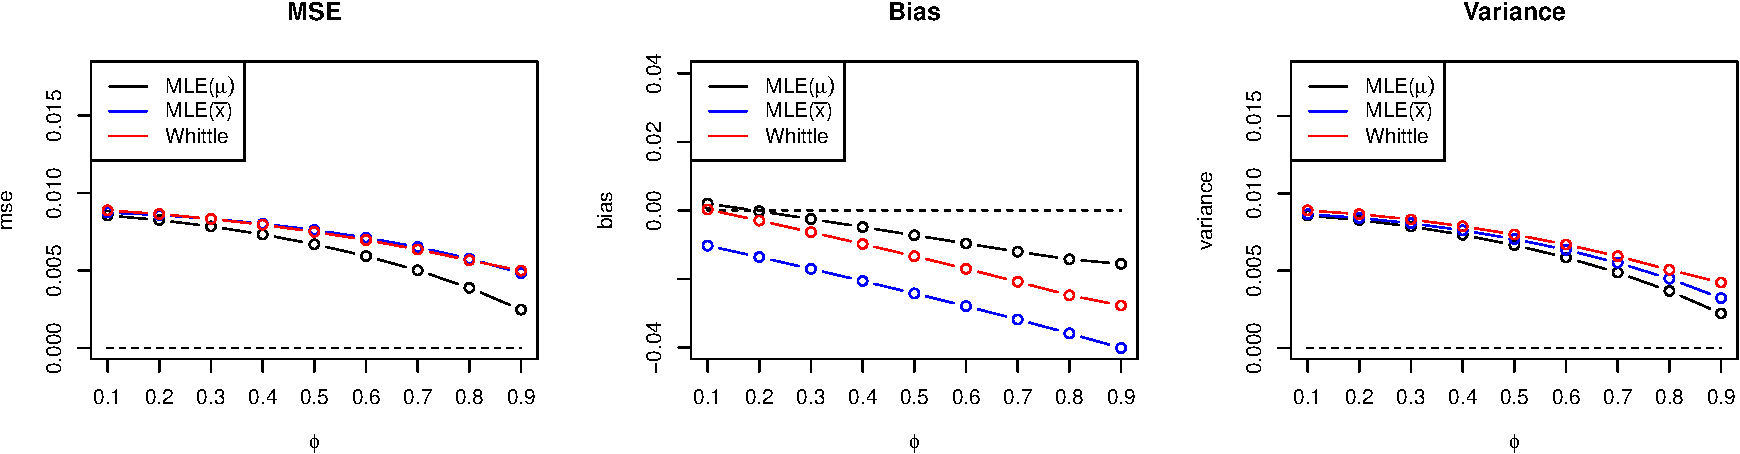
\includegraphics[width=\textwidth]{img/ar1_est_N100.pdf}
% 		\caption{$n=100$}
% 	\end{subfigure}
% 	\begin{subfigure}{\textwidth}
% 		
\includegraphics[width=\textwidth]{img/ar1_est_N1000.pdf}
% 		\caption{$n=1000$}
% 	\end{subfigure}
% 	\caption{Среднеквадратичное отклонение, смещение и дисперсия оценок параметра $\phi$ модели $\textrm{AR}(1)$ ($500$ повторений)}
% 	\label{fig:ar1_est}
% \end{figure}
% \begin{figure}[h]
% 	\centering
% 	\begin{subfigure}{\textwidth}
% 		
\includegraphics[width=\textwidth]{img/fi_est_N100.pdf}
% 		\caption{$n=100$}
% 	\end{subfigure}
% 	\begin{subfigure}{\textwidth}
% 		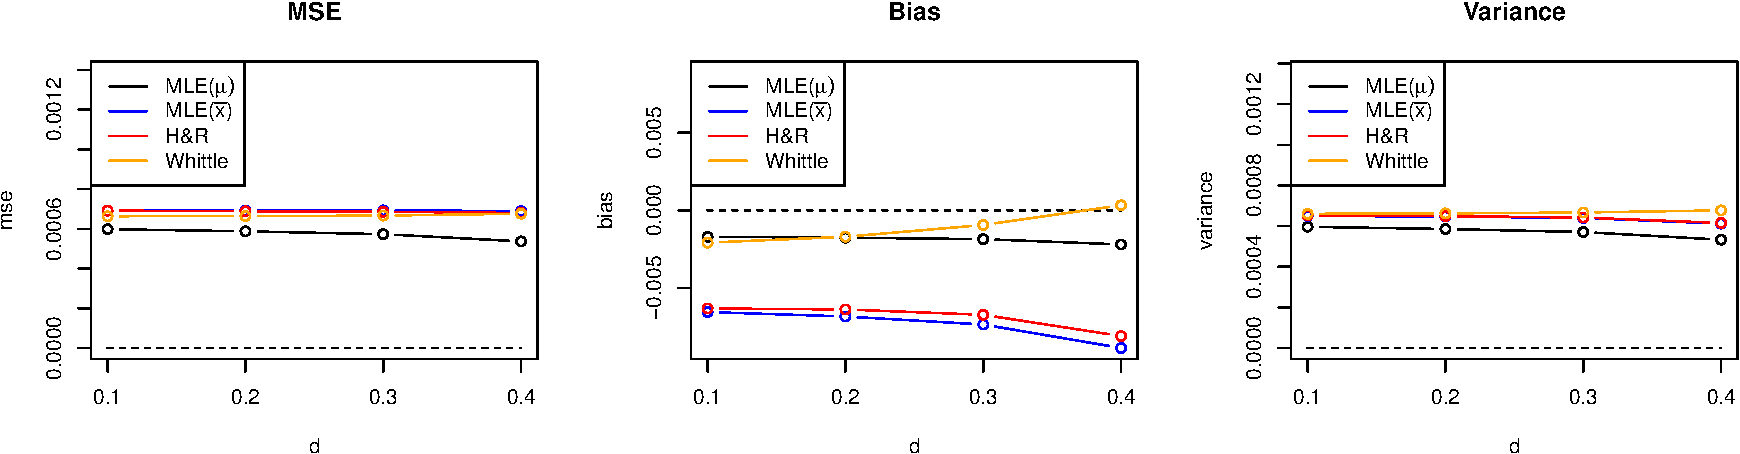
\includegraphics[width=\textwidth]{img/fi_est_N1000.pdf}
% 		\caption{$n=1000$}
% 	\end{subfigure}
% 	\caption{Среднеквадратичное отклонение, смещение и дисперсия оценок параметра $d$ модели $\textrm{ARFIMA}(0, d, 0)$ ($500$ повторений)}
% 	\label{fig:fi_est}
% \end{figure}

% На рис.~\ref{fig:ar1_est} и~\ref{fig:fi_est} изображены среднеквадратичное отклонение, смещение и дисперсия оценок параметров $\phi$ и $d$ моделей $\textrm{AR}(1)$ и $\textrm{ARFIMA}(0, d, 0)$. Отметим, что все оценки имеют в большинстве своем отрицательное смещение и отличаются между собой в основном степенью смещения. Как и ожидалось, оценка параметров методом максимального правдоподобия с известным средним дает оценку с наименьшим $\mathsf{MSE}$. С другой стороны, если использовать вместо известного среднего выборочное среднее, оценки становятся сильно смещенными. Whittle же, в свою очередь, дает менее смещенную оценку, чем $\mathrm{MLE}(\bar x)$, а в случае оценки $d$ имеет смещение даже меньше, чем у $\mathrm{MLE}(\mu)$. Однако оценки Whittle обладают наибольшей дисперсией среди всех рассмотренных методов, но разница не такая значительная, как в случае смещения.

% \begin{sidewaystable}[h!]
% 	\centering
% 	\caption{Смещение и среднеквадратичное отклонение оценок параметров $d$ и $\phi$ модели $\textrm{ARFIMA}(1, d, 0)$ ($n=100$, $500$ повторений)}
% 	\label{tab:arfi_est_n100}
% 	\scalebox{0.9}{
% 		\begin{tabular}{m{1cm}m{1cm}ccccccccm{0.2cm}cccccccc}
% 			\hline
% 			    &        & \multicolumn{8}{c}{$\mathsf{MSE}$}      &                                            & \multicolumn{8}{c}{$\mathsf{Bias}$}                                                                                                                                                                                                                                                                                                                                                                                                              \\
% 			\cline{3-10} \cline{12-19}
% 			    &        & \multicolumn{2}{c}{$\mathrm{MLE}(\mu)$} & \multicolumn{2}{c}{$\mathrm{MLE}(\bar x)$} & \multicolumn{2}{c}{H\&R}            & \multicolumn{2}{c}{Whittle} &                         & \multicolumn{2}{c}{$\mathrm{MLE}(\mu)$} & \multicolumn{2}{c}{$\mathrm{MLE}(\bar x)$} & \multicolumn{2}{c}{H\&R} & \multicolumn{2}{c}{Whittle}                                                                                                                                                                                                      \\
% 			$d$ & $\phi$ & $\hat d$                                & $\hat\phi$                                 & $\hat d$                            & $\hat\phi$                  & $\hat d$                & $\hat\phi$                              & $\hat d$                                   & $\hat\phi$               &                             & $\hat d$                 & $\hat\phi$             & $\hat d$                 & $\hat\phi$ & $\hat d$                 & $\hat\phi$              & $\hat d$                 & $\hat\phi$             \\ \hline
% 			0.1 & 0.1    & 0.049                                   & 0.056                                      & 0.119                               & 0.114                       & \textcolor{blue}{0.009} & \textcolor{red}{0.018}                  & 0.069                                      & 0.067                    &                             & -0.077                   & 0.066                  & -0.229                   & 0.199      & \textcolor{blue}{-0.054} & \textcolor{red}{0.035}  & -0.086                   & 0.068                  \\
% 			0.2 & 0.1    & 0.047                                   & 0.055                                      & 0.151                               & 0.141                       & \textcolor{blue}{0.025} & \textcolor{red}{0.032}                  & 0.077                                      & 0.073                    &                             & \textcolor{blue}{-0.078} & \textcolor{red}{0.067} & -0.265                   & 0.232      & -0.119                   & 0.099                   & -0.094                   & 0.074                  \\
% 			0.3 & 0.1    & \textcolor{blue}{0.041}                 & \textcolor{red}{0.049}                     & 0.183                               & 0.165                       & 0.049                   & 0.055                                   & 0.084                                      & 0.081                    &                             & \textcolor{blue}{-0.076} & \textcolor{red}{0.066} & -0.301                   & 0.266      & -0.179                   & 0.161                   & -0.109                   & 0.09                   \\
% 			0.4 & 0.1    & \textcolor{blue}{0.029}                 & \textcolor{red}{0.038}                     & 0.211                               & 0.187                       & 0.081                   & 0.089                                   & 0.179                                      & 0.194                    &                             & \textcolor{blue}{-0.072} & \textcolor{red}{0.065} & -0.34                    & 0.305      & -0.243                   & 0.23                    & -0.26                    & 0.241                  \\
% 			\hline
% 			0.1 & 0.5    & 0.045                                   & 0.041                                      & 0.086                               & 0.053                       & \textcolor{blue}{0.010} & \textcolor{red}{0.015}                  & 0.057                                      & 0.054                    &                             & -0.071                   & 0.034                  & -0.222                   & 0.151      & -0.07                    & 0.034                   & \textcolor{blue}{-0.066} & \textcolor{red}{0.024} \\
% 			0.2 & 0.5    & 0.042                                   & 0.038                                      & 0.092                               & 0.055                       & \textcolor{blue}{0.031} & \textcolor{red}{0.025}                  & 0.074                                      & 0.058                    &                             & \textcolor{blue}{-0.081} & \textcolor{red}{0.046} & -0.244                   & 0.171      & -0.154                   & 0.108                   & -0.153                   & 0.107                  \\
% 			0.3 & 0.5    & \textcolor{blue}{0.040}                 & \textcolor{red}{0.036}                     & 0.1                                 & 0.059                       & 0.063                   & 0.043                                   & 0.098                                      & 0.062                    &                             & \textcolor{blue}{-0.093} & \textcolor{red}{0.060} & -0.267                   & 0.192      & -0.232                   & 0.174                   & -0.209                   & 0.161                  \\
% 			0.4 & 0.5    & \textcolor{blue}{0.037}                 & \textcolor{red}{0.033}                     & 0.115                               & 0.067                       & 0.104                   & 0.065                                   & 0.104                                      & 0.066                    &                             & \textcolor{blue}{-0.103} & \textcolor{red}{0.073} & -0.304                   & 0.226      & -0.306                   & 0.235                   & -0.228                   & 0.177                  \\
% 			\hline
% 			0.1 & 0.9    & 0.029                                   & 0.029                                      & 0.014                               & 0.01                        & \textcolor{blue}{0.007} & \textcolor{red}{0.007}                  & 0.034                                      & 0.025                    &                             & 0.075                    & -0.089                 & 0.01                     & -0.049     & \textcolor{blue}{0.001}  & \textcolor{red}{-0.043} & 0.049                    & -0.069                 \\
% 			0.2 & 0.9    & 0.019                                   & 0.018                                      & 0.011                               & 0.006                       & \textcolor{blue}{0.009} & \textcolor{red}{0.004}                  & 0.026                                      & 0.019                    &                             & 0.046                    & -0.065                 & \textcolor{blue}{-0.011} & -0.035     & -0.037                   & \textcolor{red}{-0.026} & 0.02                     & -0.056                 \\
% 			0.3 & 0.9    & 0.012                                   & 0.01                                       & \textcolor{blue}{0.009}             & 0.004                       & 0.014                   & \textcolor{red}{0.003}                  & 0.022                                      & 0.015                    &                             & \textcolor{blue}{0.016}  & -0.043                 & -0.033                   & -0.023     & -0.076                   & \textcolor{red}{-0.011} & -0.024                   & -0.039                 \\
% 			0.4 & 0.9    & \textcolor{blue}{0.008}                 & 0.006                                      & 0.009                               & \textcolor{red}{0.002}      & 0.025                   & \textcolor{red}{0.002}                  & 0.028                                      & 0.01                     &                             & \textcolor{blue}{-0.016} & -0.024                 & -0.061                   & -0.008     & -0.121                   & \textcolor{red}{0.003}  & -0.095                   & -0.016                 \\ \hline
% 		\end{tabular}
% 	}
% \end{sidewaystable}

% \begin{sidewaystable}[h!]
% 	\centering
% 	\caption{Смещение и среднеквадратичное отклонение оценок параметров $d$ и $\phi$ модели $\textrm{ARFIMA}(1, d, 0)$ ($n=1000$, $500$ повторений)}
% 	\label{tab:arfi_est_n1000}
% 	\scalebox{0.9}{
% 		\begin{tabular}{m{1cm}m{1cm}ccccccccm{0.2cm}cccccccc}
% 			\hline
% 			    &        & \multicolumn{8}{c}{$\mathsf{MSE} \cdot 100$} &                                            & \multicolumn{8}{c}{$\mathsf{Bias} \cdot 100$}                                                                                                                                                                                                                                                                                                                                                                                                           \\
% 			\cline{3-10} \cline{12-19}
% 			    &        & \multicolumn{2}{c}{$\mathrm{MLE}(\mu)$}      & \multicolumn{2}{c}{$\mathrm{MLE}(\bar x)$} & \multicolumn{2}{c}{H\&R}                      & \multicolumn{2}{c}{Whittle} &                         & \multicolumn{2}{c}{$\mathrm{MLE}(\mu)$} & \multicolumn{2}{c}{$\mathrm{MLE}(\bar x)$} & \multicolumn{2}{c}{H\&R} & \multicolumn{2}{c}{Whittle}                                                                                                                                                                                                   \\
% 			$d$ & $\phi$ & $\hat d$                                     & $\hat\phi$                                 & $\hat d$                                      & $\hat\phi$                  & $\hat d$                & $\hat\phi$                              & $\hat d$                                   & $\hat\phi$               &                             & $\hat d$                 & $\hat\phi$             & $\hat d$                 & $\hat\phi$             & $\hat d$ & $\hat\phi$              & $\hat d$                 & $\hat\phi$              \\ \hline
% 			0.1 & 0.1    & \textcolor{blue}{0.186}                      & \textcolor{red}{0.290}                     & 0.27                                          & 0.37                        & 0.224                   & 0.317                                   & 0.232                                      & 0.33                     &                             & \textcolor{blue}{-0.581} & \textcolor{red}{0.448} & -1.941                   & 1.732                  & -1.729   & 1.508                   & -0.687                   & 0.519                   \\
% 			0.2 & 0.1    & \textcolor{blue}{0.181}                      & \textcolor{red}{0.287}                     & 0.271                                         & 0.371                       & 0.267                   & 0.366                                   & 0.232                                      & 0.329                    &                             & \textcolor{blue}{-0.599} & \textcolor{red}{0.465} & -2.026                   & 1.824                  & -1.981   & 1.773                   & -0.615                   & 0.468                   \\
% 			0.3 & 0.1    & \textcolor{blue}{0.174}                      & \textcolor{red}{0.282}                     & 0.272                                         & 0.372                       & 0.268                   & 0.367                                   & 0.232                                      & 0.328                    &                             & -0.639                   & 0.505                  & -2.177                   & 1.987                  & -2.176   & 1.975                   & \textcolor{blue}{-0.476} & \textcolor{red}{0.372}  \\
% 			0.4 & 0.1    & \textcolor{blue}{0.156}                      & \textcolor{red}{0.267}                     & 0.272                                         & 0.373                       & 0.274                   & 0.371                                   & 0.232                                      & 0.325                    &                             & -0.795                   & 0.666                  & -2.606                   & 2.443                  & -2.725   & 2.542                   & \textcolor{blue}{-0.263} & \textcolor{blue}{0.233} \\
% 			\hline
% 			0.1 & 0.1    & 0.761                                        & 0.8                                        & 1.429                                         & 1.3                         & \textcolor{blue}{0.504} & \textcolor{red}{0.552}                  & 1.104                                      & 1.05                     &                             & \textcolor{blue}{-2.047} & \textcolor{red}{1.588} & -5.86                    & 5.102                  & -3.256   & 2.741                   & -2.555                   & 1.904                   \\
% 			0.2 & 0.1    & \textcolor{blue}{0.710}                      & \textcolor{red}{0.759}                     & 1.432                                         & 1.302                       & 0.978                   & 0.969                                   & 1.213                                      & 1.125                    &                             & \textcolor{blue}{-2.018} & \textcolor{red}{1.571} & -6.08                    & 5.337                  & -5.157   & 4.556                   & -2.721                   & 2.065                   \\
% 			0.3 & 0.1    & \textcolor{blue}{0.617}                      & \textcolor{red}{0.675}                     & 1.462                                         & 1.323                       & 1.246                   & 1.175                                   & 1.23                                       & 1.15                     &                             & \textcolor{blue}{-1.984} & \textcolor{red}{1.560} & -6.506                   & 5.78                   & -6.129   & 5.463                   & -2.578                   & 1.948                   \\
% 			0.4 & 0.1    & \textcolor{blue}{0.473}                      & \textcolor{red}{0.539}                     & 1.499                                         & 1.353                       & 1.507                   & 1.354                                   & 1.294                                      & 1.18                     &                             & \textcolor{blue}{-2.226} & \textcolor{red}{1.861} & -7.514                   & 6.838                  & -7.622   & 6.905                   & -2.695                   & 2.099                   \\
% 			\hline
% 			0.1 & 0.9    & 0.338                                        & 0.155                                      & 0.288                                         & 0.122                       & \textcolor{blue}{0.259} & \textcolor{red}{0.097}                  & 0.387                                      & 0.193                    &                             & 0.623                    & -0.774                 & \textcolor{blue}{-0.095} & -0.56                  & -0.176   & \textcolor{red}{-0.504} & 0.583                    & -0.92                   \\
% 			0.2 & 0.9    & 0.273                                        & 0.106                                      & \textcolor{blue}{0.233}                       & \textcolor{red}{0.077}      & 0.239                   & 0.077                                   & 0.326                                      & 0.128                    &                             & 0.42                     & -0.611                 & -0.388                   & -0.355                 & -0.627   & \textcolor{red}{-0.303} & \textcolor{blue}{0.041}  & -0.652                  \\
% 			0.3 & 0.9    & 0.241                                        & 0.093                                      & \textcolor{blue}{0.217}                       & \textcolor{red}{0.068}      & 0.268                   & 0.075                                   & 0.326                                      & 0.097                    &                             & \textcolor{blue}{0.287}  & -0.53                  & -0.667                   & -0.204                 & -1.395   & \textcolor{red}{-0.029} & -1.003                   & -0.285                  \\
% 			0.4 & 0.9    & \textcolor{blue}{0.173}                      & 0.067                                      & 0.182                                         & \textcolor{red}{0.051}      & 0.381                   & 0.076                                   & 0.545                                      & 0.09                     &                             & \textcolor{blue}{-0.129} & -0.295                 & -1.4                     & \textcolor{red}{0.178} & -2.602   & 0.359                   & -3.357                   & 0.389                   \\
% 			\hline
% 		\end{tabular}
% 	}
% \end{sidewaystable}

% В таблицах~\ref{tab:arfi_est_n100} и~\ref{tab:arfi_est_n1000} представлены значения среднеквадратичной ошибки и смещения оценок параметров $d$ и $\phi$ модели $\textrm{ARFIMA}(1, d)$. Заметим, что в оценках присутствует смещение, для $\phi=0.1$ и $\phi=0.5$ оценки $d$ имеют отрицательное смещение, а оценки $\phi$, наоборот, положительное. Также в таблицах синим цветом выделена лучшая по строке оценка $d$, а красным~--- лучшая оценка $\phi$. Видно, что в случае коротких рядов ($n=100$) метод H\&R в большинстве случаев дает оценки с наименьшим $\mathsf{MSE}$, однако наименьшее смещение имеют оценки $\mathrm{MLE}(\mu)$. В случае же длинных рядов ($n=1000$) наименьшую среднеквадратичную ошибку и смещение дает $\mathrm{MLE}(\mu)$. Отметим, что даже для длинных рядов оценки $\mathrm{MLE}(\bar x)$ имеют, в большинстве случаев, наибольшее смещение и $\mathsf{MSE}$. Оценки H\&R, хотя и дают наименьшее после $\mathrm{MLE}(\mu)$ $\mathsf{MSE}$, также сильно смещены. Оценки методом Whittle выглядят наиболее привлекательными, поскольку имеют наименьшее после $\mathrm{MLE}(\mu)$ смещение и имеют $\mathsf{MSE}$ меньше, чем $\mathrm{MLE}(\bar x)$.

% Подведем итоги численного сравнения. Если для рассматриваемого ряда известно его матожидание $\mu$ (что, конечно, редкость на практике), наилучшим методом является $\mathrm{MLE}(\mu)$. Если же среднее неизвестно, для коротких рядов оценивать параметры моделей $\textrm{AR}(1)$ и $\textrm{ARFIMA}(0, d, 0)$ следует методом Whittle, а параметры модели $\textrm{ARFIMA}(1, d, 0)$~--- методом H\&R. В случае длинных рядов параметры рассматриваемых моделей следует оценивать методом Whittle.

% % \begin{table}[h!]
% % 	\centering
% % 	\caption{Смещение и среднеквадратичное отклонение оценок параметра $\phi$ модели $\textrm{AR}(1)$ ($n=100$, $500$ повторений)}
% % 	\begin{tabular}{m{1cm}cccm{0.5cm}ccc}
% % 		\hline
% % 		& \multicolumn{3}{c}{$\mathsf{bias}\cdot 100$} & & \multicolumn{3}{c}{$\mathsf{MSE}\cdot 100$} \\
% % 		\cline{2-4} \cline{6-8}
% % 		$\phi$ & $\mathrm{MLE}(\mu)$ & $\mathrm{MLE}(\bar x)$ & Whittle & & $\mathrm{MLE}(\mu)$ & $\mathrm{MLE}(\bar x)$ & Whittle \\ \hline
% % 		0.1 & 0.197  & -1.029 &  0.025 & & 0.856 & 0.874 & 0.889\\
% % 		0.2 & -0.023 & -1.362 & -0.298 & & 0.826 & 0.859 & 0.865\\
% % 		0.3 & -0.252 & -1.707 & -0.635 & & 0.785 & 0.834 & 0.834\\
% % 		0.4 & -0.487 & -2.061 & -0.981 & & 0.733 & 0.802 & 0.796\\
% % 		0.5 & -0.725 & -2.423 & -1.337 & & 0.670 & 0.762 & 0.75\\
% % 		0.6 & -0.965 & -2.796 & -1.704 & & 0.594 & 0.712 & 0.697\\
% % 		0.7 & -1.205 & -3.183 & -2.084 & & 0.502 & 0.652 & 0.636\\
% % 		0.8 & -1.427 & -3.59  & -2.478 & & 0.389 & 0.577 & 0.566\\
% % 		0.9 & -1.560 & -4.016 & -2.777 & & 0.248 & 0.483 & 0.5\\
% % 		\hline
% % 	\end{tabular}
% % \end{table}

% \subsection{Сходимость оценок к истинным значениям}
% Известно~\cite[Theorem 8.1]{Hassler2018}, что
% \begin{equation}\label{eq:mle_distribution}
% 	\sqrt{n}(\widehat{\bm\varphi}_\mathrm{ML} - \bm\varphi_0)\overset{d}{\longrightarrow} \mathcal{N}_{k+1}(0, \mathcal{I}^{-1}(\bm{\varphi}_0)),
% \end{equation}
% где $\bm\varphi_0$~--- истинный вектор параметров, $\mathcal{I}(\bm\varphi)$~--- информационная матрица Фишера. Также известно~\cite[Proposition 8.3]{Hassler2018}, что вектор $\widehat{\bm\varphi}_W$ имеет такое же асимптотическое распределение, что и $\widehat{\bm\varphi}_\mathrm{ML}$.

% Покажем, что методы $\mathrm{MLE}(\mu)$ и Whittle реализованы корректно, посмотрев на дисперсию оценок для $n=10000$. В таблице~\ref{tab:variance} представлены оценки дисперсий $\hat d$ и $\hat \phi$, в скобках указана теоретическая дисперсия. Как видим, для разных значений параметров значение дисперсий оценок близки к теоретическим.

% \begin{table}[h]
% 	\centering
% 	\subfloat[$d=0.2$, $\varphi=0.1$]{
% 		\begin{tabular}{c|cc}
% 			Метод               & $n\mathsf{D} \hat d$ (1.83167) & $n\mathsf{D}\hat \phi$ (2.98284) \\
% 			\hline
% 			$\mathrm{MLE}(\mu)$ & 1.72733                        & 2.92604                          \\
% 			Whittle             & 1.78350                        & 2.94929                          \\
% 			\hline
% 		\end{tabular}
% 	}
% 	\subfloat[$d=0.4$, $\varphi=0.1$]{
% 		\begin{tabular}{c|cc}
% 			Метод               & $n\mathsf{D} \hat d$ (1.83167) & $n\mathsf{D}\hat \phi$ (2.98284) \\
% 			\hline
% 			$\mathrm{MLE}(\mu)$ & 1.69348                        & 2.90374                          \\
% 			Whittle             & 1.84265                        & 2.96828                          \\
% 			\hline
% 		\end{tabular}
% 	}\vspace{2em}
% 	\subfloat[$d=0.2$, $\varphi=0.5$]{
% 		\begin{tabular}{c|cc}
% 			Метод               & $n\mathsf{D} \hat d$ (4.91219) & $n\mathsf{D}\hat \phi$ (6.06018) \\
% 			\hline
% 			$\mathrm{MLE}(\mu)$ & 5.00869                        & 6.305                            \\
% 			Whittle             & 5.08405                        & 6.35985                          \\
% 			\hline
% 		\end{tabular}
% 	}
% 	\subfloat[$d=0.4$, $\varphi=0.5$]{
% 		\begin{tabular}{c|cc}
% 			Метод               & $n\mathsf{D} \hat d$ (4.91219) & $n\mathsf{D}\hat \phi$ (6.06018) \\
% 			\hline
% 			$\mathrm{MLE}(\mu)$ & 4.75975                        & 6.06711                          \\
% 			Whittle             & 5.28104                        & 6.4936                           \\
% 			\hline
% 		\end{tabular}
% 	}\vspace{2em}
% 	\subfloat[$d=0.2$, $\varphi=0.9$]{
% 		\begin{tabular}{c|cc}
% 			Метод               & $n \mathsf{D} \hat d$ (2.49203) & $n\mathsf{D}\hat \phi$ (0.77885) \\
% 			\hline
% 			$\mathrm{MLE}(\mu)$ & 2.42011                         & 0.78209                          \\
% 			Whittle             & 2.44394                         & 0.77549                          \\
% 			\hline
% 		\end{tabular}
% 	}
% 	\subfloat[$d=0.4$, $\varphi=0.9$]{
% 		\begin{tabular}{c|cc}
% 			Метод               & $n \mathsf{D} \hat d$ (2.49203) & $n\mathsf{D}\hat \phi$ (0.77885) \\
% 			\hline
% 			$\mathrm{MLE}(\mu)$ & 2.26718                         & 0.749318                         \\
% 			Whittle             & 2.57117                         & 0.77311                          \\
% 			\hline
% 		\end{tabular}
% 	}
% 	\caption{Дисперсия оценок $\hat d$ и $\hat \phi$, $n=10000$, $100$ повторений}
% 	\label{tab:variance}
% \end{table}

\chapter{Метод Monte Carlo SSA}\label{chpt:mcssa}

\section{Вспомогательные определения}

Для начала введем некоторые обозначения теории случайных процессов, которые будем использовать в дальнейшем.
\begin{definition}\label{def:stationary}
	Случайный процесс $\{Y_t:t\in\mathbb{Z}\}$ называют стационарным (в широком смысле), если
	\begin{enumerate}
		\item $\mathsf{E}Y_t\equiv\const$ (среднее постоянно по времени);
		\item $\mathsf{cov}(Y_t,Y_{t+h})=\gamma(h)$ (ковариация зависит только от лага $h$).
	\end{enumerate}
\end{definition}
\begin{remark}
	Поскольку $\gamma(0)=\mathsf{cov}(Y_t,Y_t)=\mathsf{D}Y_t$, то дисперсия также не меняется со временем.
\end{remark}
\begin{remark}
	Далее под стационарностью будет подразумеваться именно стационарность в широком смысле.
\end{remark}
\begin{definition}
	Случайный процесс $\{\varepsilon_t\}$ называют белым шумом $\mathrm{WN}(0, \sigma^2)$, если он стационарный, $\mathsf{E}\varepsilon_t=0$, $\gamma(h)=0$ $\forall h\ne 0$ и $\mathsf{D}\varepsilon_t=\sigma^2$.
\end{definition}

\begin{definition}
	Моделью $\mathrm{ARMA}(p, q)$, где $p$, $q\in \mathbb{N}\cup\{0\}$ называют случайный процесс $\{X_t\}$, удовлетворяющий соотношению
	\[
		X_t=\varepsilon_t + \sum_{i=1}^p \phi_i X_{t-i} + \sum_{i=1}^q\theta_i\varepsilon_{t-i},
	\]
	где $\{\varepsilon_t\}\sim\mathrm{WN}(0, \sigma^2)$.
\end{definition}
\begin{remark}
	Модель $\mathrm{ARMA}(p, q)$ является стационарным и обратимым процессом, если корни характеристических полиномов
	\[
		\Phi(L)=1-\sum_{i=1}^p \phi_i L^i,\quad \Theta(L)=1+\sum_{i=1}^q \theta_i L^i
	\]
	лежат вне единичной окружности $\{z:|z|=1\}$~\cite[Section 3.4.1]{BoxJenkins2016}.
\end{remark}

\begin{definition}
	Процесс $\{X_t\}$ называют красным шумом с параметрами $\phi$ и $\sigma^2$, если $\{X_t\}$~--- стационарная модель $\mathrm{ARMA}(p, q)$ с $p=1$, $q=0$ и $\phi=\phi_1\in(0, 1)$.
\end{definition}

\begin{definition}
	Спектральной плотностью стационарного процесса называется такая функция $f(\omega)$, что
	\[
		\gamma(h)=\int_{0}^{1} e^{2\pi h\omega\im}f(\omega)d\omega.
	\]
\end{definition}
\begin{definition}
	Пусть $\{Y_t\}$~--- стационарный процесс. Функцию
	\begin{equation}\label{eq:pgram}
		I(\omega)=\frac1n\left|\sum_{j=1}^{n} Y_je^{-2\pi \omega (j-1)\mathrm{i}}\right|^2
	\end{equation}
	называют периодограммой выборки размера $n$ процесса $\{Y_t\}$.
\end{definition}
\begin{remark}
	Для любой фиксированной частоты $\omega_0$
	\begin{align*}
		\mathsf{E}\left(I(\omega_0)\right)\to f(\omega_0),\quad       & n\to \infty; \\
		\mathsf{D}\left(I(\omega_0)\right)\to f^2(\omega_0)\ne0,\quad & n\to\infty.
	\end{align*}
	Таким образом периодограмма является асимптотически несмещенной, но несостоятельной, оценкой спектральной плотности~\cite[Раздел 4.5]{Hassler2018}.
\end{remark}

\section{Проверка статистических гипотез}

Рассмотрим некоторый критерий со статистикой $T$. Введем обозначения.
% \begin{definition}
% 	p-value~--- такое значение $\mathrm p$, что при значениях уровня значимости $\alpha$, больших $\mathrm p$, $H_0$ отвергается (статистика попадает в критическую область $A_\text{крит}(\alpha)$), а при меньших~--- не отвергается.
% \end{definition}
\begin{definition}
	Ошибка первого рода~--- вероятность отвергнуть нулевую гипотезу, если она верна: $\alpha_I(\alpha)=\mathsf P_{H_0}(T\in A_\text{крит}(\alpha))$.
\end{definition}
\begin{definition}
	Если $\alpha_I=\alpha$, то говорят, что критерий точный при уровне значимости $\alpha$, иначе говорят, что критерий неточный. При $\alpha_I<\alpha$ критерий является консервативным, а при $\alpha_I>\alpha$~--- радикальным.
\end{definition}
\begin{definition}
	Мощность критерия против альтернативы $H_1$~--- вероятность отвергнуть нулевую гипотезу, если верна альтернативная: $\beta(\alpha)=\mathsf P_{H_1}(T\in A_\text{крит}(\alpha))$.
\end{definition}
% \begin{remark}
% 	По определению p-value $\alpha_I(\alpha)=\mathsf P_{H_0}(\mathrm p < \alpha)$ и $\beta(\alpha)=\mathsf P_{H_1}(\mathrm p < \alpha)$.
% \end{remark}

\subsection{Поправка неточных критериев}\label{sect:correction}
Зафиксируем некоторый неточный (консервативный или радикальный) критерий и уровень значимости $\alpha^*$. Пусть дана зависимость ошибки первого рода от уровня значимости $\alpha_I(\alpha)=\mathsf P_{H_0}(\mathrm p < \alpha)$. Тогда критерий с формальным уровнем значимости $\widetilde\alpha^*=\alpha_I^{-1}(\alpha^*)$ является точным: ошибка первого рода $\alpha_I(\widetilde\alpha^*)=\alpha^*$.

Если зависимость $\alpha_I(\alpha)$ неизвестна, она оценивается с помощью моделирования. Приведем алгоритм поправки в этом случае.
\begin{algorithm}
	\caption{Поправка уровня значимости по зависимости $\alpha_I(\alpha)$~\cite{Larin2022}\label{alg:correction}}
	\Input неточный критерий, уровень значимости $\alpha$, количество выборок $M$ для оценки $\alpha_I(\alpha)$ и их объем $N$.\\
	\Output формальный уровень значимости $\widetilde{\alpha}^*$.
	\begin{algorithmic}[1]
		\State Моделируется $M$ выборок объема $N$ при верной $H_0$.
		\State По моделированным данным строится оценка зависимость ошибки первого рода от уровня значимости $\alpha_I(\alpha)$.
		\State Рассчитывается формальный уровень значимости: $\widetilde{\alpha}^*=\alpha_I^{-1}(\alpha^*)$. Критерий с таким уровнем значимости является асимптотически точным при $M\to\infty$.
	\end{algorithmic}
\end{algorithm}

\subsection{Сравнение критериев}
Точные критерии, проверяющие одну и ту же гипотезу, можно использовать и сравнивать по мощности: чем больше мощность, тем лучше. Если критерий является консервативным, использовать и сравнивать его с другими критерии по мощности также можно, учитывая, что его мощность будет занижена. Радикальный же критерий, без поправки, введенной в разделе~\ref{sect:correction}, нельзя использовать и сравнивать по мощности с другими критериями. Поэтому введем понятие ROC-кривой, соответствующее мощности критерия, к которому была применена поправка.
\begin{definition}
	ROC-кривая~--- это кривая, задаваемая параметрически
	\[
		\begin{cases}
			x=\alpha_I(\alpha) \\
			y=\beta(\alpha)
		\end{cases},\quad \alpha\in[0,1]
	\]
\end{definition}
\begin{remark}
	С помощью ROC-кривых можно сравнивать по мощности неточные (в частности, радикальные) критерии. Отметим, что для точного критерия ROC-кривая совпадает с графиком мощности, так как $\alpha_I(\alpha)=\alpha$.
\end{remark}

\section{Monte Carlo SSA}\label{sect:mcssa}

Метод Monte Carlo SSA (MC-SSA) тесно связан с методом SSA (Singular Spectrum Analysis), состоящим из четырех этапов: \emph{вложения}, \emph{разложения}, \emph{группировки} и \emph{диагонального усреднения}. Поэтому опишем сначала его.
\subsection{Метод SSA}
Пусть $\tX=(x_1,\ldots,x_N)$~--- временной ряд длины $N$. Зафиксируем длину окна $L$, $1<L<N$. Рассмотрим $K=N-L+1$ векторов вложения $X_i=(x_i,\ldots,x_{i+L-1})$ и составим из столбцов $X_i$ так называемую траекторную матрицу:
\[
	\bfX = [X_1:\ldots:X_K].
\]
Далее траекторная матрица $\bfX$ разбивается в сумму матриц единичного ранга. В базовом SSA используются собственные векторы матрицы $\bfX\bfX^\rmT$, в Toeplitz SSA используются собственные векторы матрицы $\bfT$ с элементами
\begin{equation}\label{eq:toeplitz}
	t_{ij} = \frac{1}{N - |i - j|}\sum_{n=1}^{N - |i - j|}x_n x_{n+|i-j|},\quad i,j\leqslant L.
\end{equation}
Обозначим за $P_1,\ldots,P_L$ собственные векторы матрицы $\bfX\bfX^\rmT$ либо матрицы $\bfT$. Тогда получаем следующее разложение:
\[
	\bfX = \sum_{i=1}^L \sigma_i P_i Q_i^\rmT = \bfX_1+\ldots+\bfX_L,
\]
где $S_i=\bfX^\rmT P_i$, $Q_i=S_i/\|S_i\|$, $\sigma_i=\|S_i\|$.

После этого полученные матрицы группируются и каждая из группированных матриц преобразовывается обратно во временной ряд. Таким образом, результатом SSA является разложение временного ряда.
\subsection{Постановка задачи}
Рассмотрим задачу поиска сигнала (неслучайной составляющей) во временном ряде. Модель выглядит следующим образом:
\[
	\tX=\tS + \bm\xi,
\]
где $\tS$~--- сигнал, $\bm\xi$~--- стационарный в широком смысле (см. определение~\ref{def:stationary}) процесс с нулевым средним. Тогда нулевая гипотеза $H_0:\tS=0$ (отсутствие сигнала, ряд состоит из чистого шума) и альтернатива $H_1:\tS\ne0$ (ряд содержит сигнал, например, периодическую составляющую).

\subsection{Множественный тест}\label{sect:multiple_test}
% Зафиксируем длину окна $L$ и модель шума $\bm\xi$. Пусть $\tR_1, \ldots, \tR_G$~--- реализации $\bm\xi$, которые в дальнейшем будем называть суррогатными. Обозначим за $\bfX$ и $\bm\Xi_i$, $i=1,\ldots, G$, траекторные матрицы ряда $\tX$ и каждой суррогатной реализации соответственно.
Рассмотрим $H$ проекционных векторов $W_1,\ldots,W_H$, каждый из которых соответствует некоторой частоте $\omega_k$, $\|W_k\|=1$, $k=1,\ldots,H$. Приведем в алгоритме~\ref{alg:multiple_mc-ssa} метод Multiple MC-SSA~\cite{Golyandina2023}, который далее будем для простоты называть MC-SSA.
\begin{algorithm}[!ht]
	\caption{Multiple MC-SSA~\cite{Golyandina2023}}\label{alg:multiple_mc-ssa}
	\Input временной ряд $\tX$, длина окна $L$, набор векторов $W_k\in \R^L$, $\|W_k\|=1$, $k=1,\ldots, H$, модель шума $\bm\xi$, уровень значимости $\alpha$, количество суррогатных реализаций $G$.\\
	\Output $H_0$ отвергается/не отвергается, скорректированные интервалы прогнозирования
	\begin{algorithmic}[1]
		\State Сгенерировать $G$ реализаций процесса $\bm\xi$, обозначим их за $\tR_1, \ldots, \tR_G$. Обозначим за $\bm\Xi_i$ соответствующие им траекторные матрицы.
		\State Для $k=1,\dots,H$ вычислить статистику $\widehat{p}_k=\|\bfX^\rmT W_k\|^2$, выборку $P_k=\{p_{ki}\}_{i=1}^G$ с элементами $p_{ki}=\|\bm\Xi_i^\rmT W_k\|^2$, ее среднее $\mu_k$ и стандартное отклонение $\sigma_k$.
		\State Вычислить $\mathbf{\eta}=(\eta_1,\dots,\eta_G)$, где
		\[
			\eta_i=\max_{1\leqslant k\leqslant H}(p_{ki}-\mu_k)/\sigma_k,\quad i=1,\dots,G.
		\]
		\State Найти $q$ как выборочный $(1-\alpha)$-квантиль $\eta$, где $\alpha$~--- уровень значимости.
		\State Нулевая гипотеза не отвергается, если
		\[
			t = \max_{1\leqslant k\leqslant H}(\widehat{p}_k-\mu_k)/\sigma_k<q.
		\]
		\State Если $H_0$ отвергнута, вклад $W_k$ (и соответствующей частоты) значим, если $\widehat{p}_k$ превосходит $\mu_k+q\sigma_k$. Таким образом, $[0,\mu_k+q\sigma_k]$~--- скорректированные интервалы прогнозирования.
	\end{algorithmic}
\end{algorithm}

\subsection{Используемый вариант MC-SSA}\label{sect:vectors_choise}
В разделе~\ref{sect:multiple_test} предполагалось, что векторы $W_1,\ldots, W_H$ фиксированные и не зависят от исходного ряда. Такой критерий MC-SSA является точным, то есть ошибка первого рода равна заданному уровню значимости. В этой работе будут рассматриваться векторы $W_k$, порожденные рядом $\tX$, при этом по-прежнему при вычислении $p_{ki}$ используются те же $W_k$, что и при вычислении $\widehat p_k$.
% \begin{remark}\label{remark:complexity}
% 	Если критерий MC-SSA точный и не требует поправки, то его трудоемкость состоит из трудоемкости одного разложения траекторной матрицы исходного ряда и $G$ вычислений по формуле~\eqref{eq:mc-ssa_h0}. При применении поправки трудоемкость увеличивается в $M$ раз, где $M$~--- количество выборок для оценки зависимости $\alpha_I(\alpha)$.
% \end{remark}

Поскольку в этом варианте векторы $W_k$ не заданы заранее, а порождены исходным рядом, критерий MC-SSA становится, вообще говоря, радикальным. Бороться с этой проблемой позволяет метод эмпирической поправки критерия, описанный в разделе~\ref{sect:correction}.

В качестве $W_1, \ldots,W_H$ будем брать собственные векторы матрицы $\bfX\bfX^\rmT$ или $\bfT$~\eqref{eq:toeplitz} в зависимости от того, является ли рассматриваемый ряд стационарным в широком смысле (определение~\ref{def:stationary}). Такой способ выбора векторов для проекции самый распространенный, поскольку, если есть значимые векторы, можно восстановить сигнал с помощью SSA на их основе. Будем под MC-SSA подразумевать именно этот вариант критерия. Варианты критерия будут определяться конкретным разложением траекторной матрицы. Заметим, что обычно используется сингулярное разложение.

\subsection{Ограничение на модель шума}\label{sect:noise_constraint}

Заметим, что при верной $H_0:\tS=0$ верно следующее:
\[
\operatorname*{plim}_{K\to\infty}\bfX\bfX^\rmT / K = \Sigma_L,\quad \operatorname*{plim}_{K\to\infty}\bfT = \Sigma_L.
\]
где $\Sigma_L=(\gamma(|i-j|))_{i,j=1}^L$~--- $L$-ковариационная матрица процесса $\bm\xi$. Поэтому собственные векторы матрицы $\bfX\bfX^\rmT$ (и $\bfT$) асимптотически стремятся к собственным векторам $\Sigma_L$.

В связи с этим для выбранного варианта MC-SSA возникает ограничение на модель шума $\bm\xi$: спектральная плотность процесса должна быть строго монотонной. Это связано с тем, что в таком случае собственные векторы автоковариационной матрицы стационарного процесса ведут себя как синусоиды с равностоящими частотами, а соответствующие им собственные числа примерно равны значению спектральной плотности в этих частотах. Для процессов с короткой памятью это верно, поскольку теплицеву симметричную матрицу можно аппроксимировать циркулянтной матрицей~\cite{Gray2005}, собственные векторы которой равны
\[
	v_j=\frac{1}{\sqrt n}\left(1, \omega^j, \omega^{2j},\ldots,\omega^{(n-1)j}\right),\quad j=0,1\ldots,n-1,
\]
а соответствующие им собственные числа равны
\[
	\lambda_j = \sum_{k=0}^{n-1}c_k\omega^{j},
\]
где $\omega=\exp\{2\pi\im / n\}$. Тогда при строгой монотонности $f_{\bm\xi}(\omega)$ вклад собственных векторов будет попарно различным, делая их сильно разделимыми~\cite[Раздел 1.5.4]{Golyandina2001}. Если же опустить требование строгой монотонности, компоненты могут смешаться, что сделает невозможным определение доминирующей частоты значимого вектора.
% \begin{remark}
% 	Примерами процессов со строго монотонной спектральной плотностью являются красный шум и модель $\textrm{ARFIMA}(0, d, 0)$.
% \end{remark}

Для процессов с длинной памятью покажем правдивость этого факта, проведя численный эксперимент. Рассмотрим модель $\textrm{ARFIMA}(0, d, 0)$ с $d=0.4$ и пусть размер автоковариационной матрицы $\bm\Sigma_n$ равен $n=100$. Частоту векторов будем оценивать с помощью метода \textsf{ESPRIT}~\cite[Раздел 3.1]{SSA_R}.

\begin{figure}[h]
	\begin{subfigure}{\textwidth}
		
\includegraphics[width=\textwidth]{img/eigenvectors_longmemo1.pdf}
	\end{subfigure}
	\begin{subfigure}{\textwidth}
		
\includegraphics[width=\textwidth]{img/eigenvectors_longmemo2.pdf}
	\end{subfigure}
	\caption{Собственные векторы автоковариационной матрицы модели $\textrm{ARFIMA}(0, d, 0)$}
	\label{fig:eigenvectors_longmemo}
\end{figure}

\begin{figure}[h]
	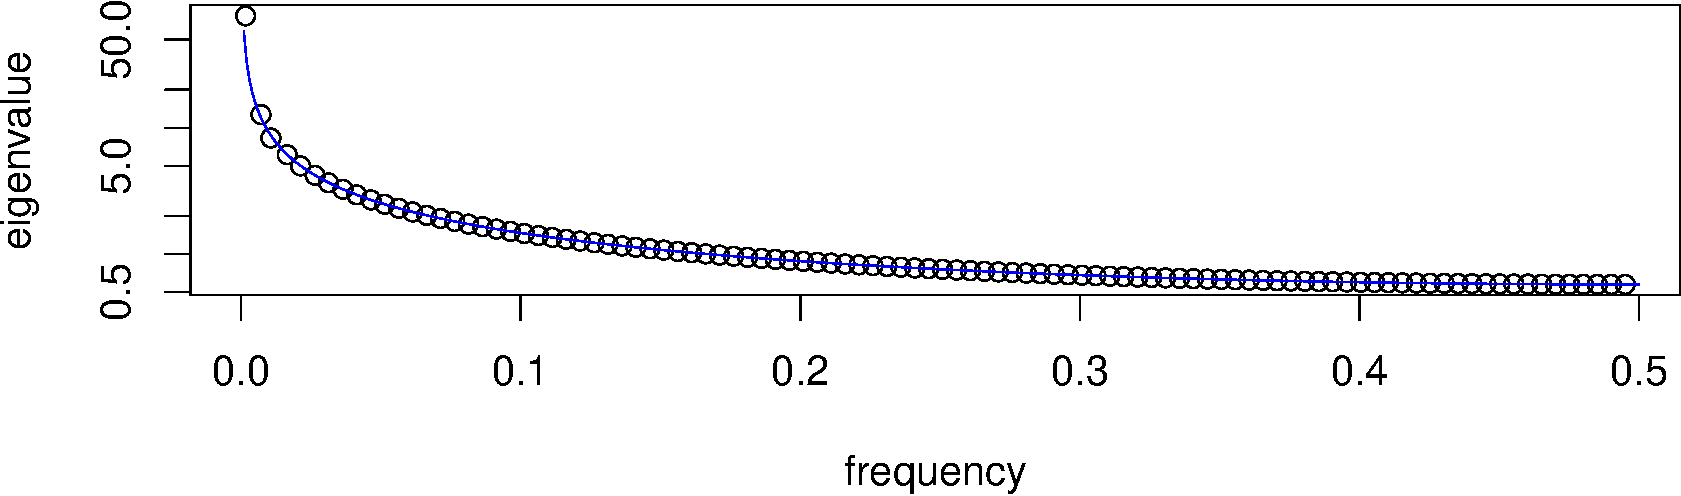
\includegraphics[width=\textwidth]{img/eigenvalues_longmemo.pdf}
	\caption{Собственные числа автоковариационной матрицы модели $\textrm{ARFIMA}(0, d, 0)$}
	\label{fig:eigenvalues_longmemo}
\end{figure}

\begin{figure}[h]
	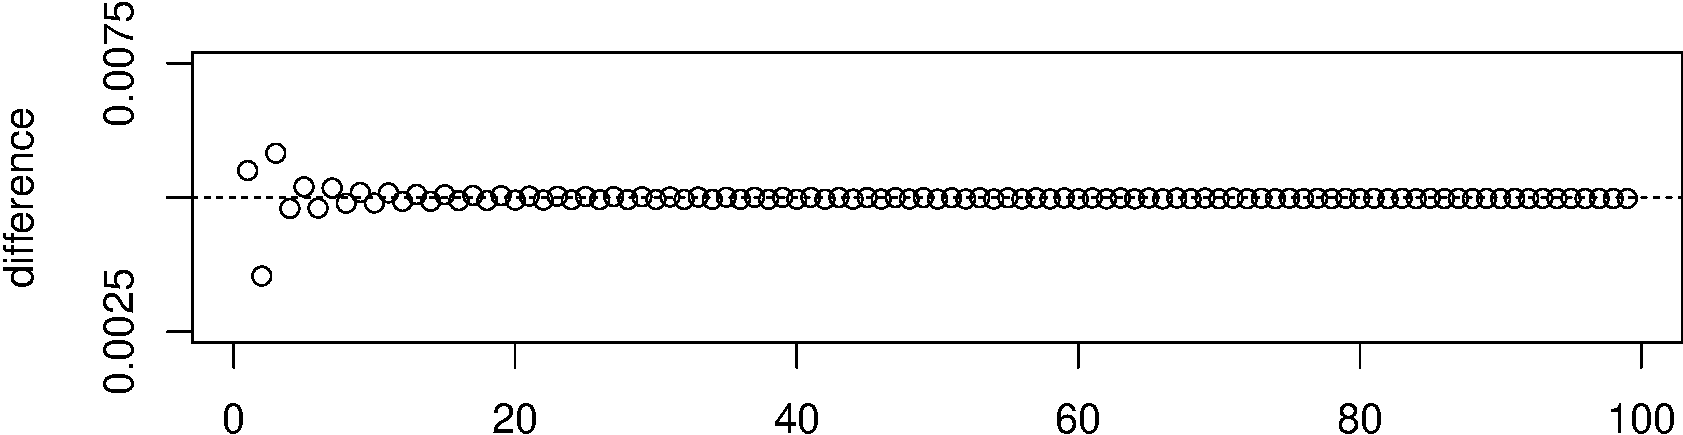
\includegraphics[width=\textwidth]{img/eigenvectors_freq_diff.pdf}
	\caption{Разница частот между ближайшими собственными векторами}
	\label{fig:freq_diff}
\end{figure}

На рис.~\ref{fig:eigenvectors_longmemo} представлены первые $10$ собственных векторов матрицы $\bm\Sigma_n$, на рис.~\ref{fig:eigenvalues_longmemo} по оси $Ox$ отложена частота, которой соответствует собственный вектор, а по оси $Oy$ отложено соответствующее вектору собственное число, дополнительно синей линией проведена спектральная плотность процесса. Как видим, действительно, собственные векторы ведут себя как периодики, собственные числа хорошо приближаются значением спектральной плотности в соответствующей частоте, и по рис.~\ref{fig:freq_diff} разница между частотами примерно равна $1 / (2n)=0.005$.

В случае, когда спектр шума не монотонный, возникают одинаковые собственные числа, которые образуют собственное подпространство, любой вектор из которого является собственным. Таким образом уже нельзя быть уверенным в том, что вектору соответствует определенная частота. Этот недостаток ограничивает использование MC-SSA для большого класса процессов, в частности, для белого шума. 

\subsection{Сравнение способов задания проекционных векторов}\label{sect:mcssa_comp}

Сравним численно два способа задания векторов для проекции $W_k$ критерия MC-SSA (алгоритм~\ref{alg:multiple_mc-ssa}):
\begin{enumerate}
	\item Собственные векторы матрицы $\bfX\bfX^\rmT$ или $\bfT$~\eqref{eq:toeplitz} (см. раздел~\ref{sect:vectors_choise}).
	\item Поскольку для стационарных процессов собственные векторы $L$-ковариационной матрицы $\Sigma_L$ представляют собой гармоники с равноотстоящими частотами (см. раздел~\ref{sect:noise_constraint}), рассмотрим косинусы с равноотстоящими частотами:
	      \begin{equation}\label{eq:cos_proj_vectors}
		      V_k=
		      \begin{pmatrix}
			      \cos(2\pi\omega_k 1) \\
			      \ldots               \\
			      \cos(2\pi\omega_k L)
		      \end{pmatrix},\quad W_k=\frac{V_k}{\|V_k\|},\quad k=1,\ldots,L,
	      \end{equation}
	      где $\omega_k=k / (2L)$.
\end{enumerate}
Для краткости будем называть соответствующие им критерии MC-SSA <<ev>> и <<cos>> соответственно.

Введем понятие соотношения сигнал-шум. Обычно под ним понимают соотношение
\begin{equation}\label{eq:snr_wn}
	\frac{\sum\limits_{n=1}^N s^2_n/N}{\mathsf{D}{\bm\xi}},
\end{equation}
где $\mathsf{S}=(s_1,\ldots,s_N)$~--- сигнал, $\bm{\xi}$~--- шум. Но, поскольку это определение не учитывает поведение спектральной плотности шума, обобщим его.

\begin{definition}
	Будем называть
	\begin{equation}\label{eq:snr}
		\operatorname{SNR}(\mathsf{S}, \bm\xi)=\frac1N\sum_{j=0}^{N-1}\frac{I(j/N)}{f_{\bm{\xi}}(j/N)}
	\end{equation}
	соотношением сигнал-шум, где $I(\omega)$~--- периодограмма~\eqref{eq:pgram} временного ряда $\tS$, $f_{\bm\xi}(\omega)$~--- спектральная плотность процесса $\bm\xi$.
\end{definition}

\begin{remark}
	Для белого шума с плотностью $f_{\bm\xi}(\omega)=\sigma^2$ формулы~\eqref{eq:snr_wn} и~\eqref{eq:snr} совпадают.
\end{remark}

Будем рассматривать ряды длины $N=100$ и $L\in\{10,20,50,80,90\}$. В качестве альтернативы рассмотрим
\begin{equation}\label{eq:em_harmonic}
	\mathsf{S}=\left\{Ae^{a n}\cos(2\pi\omega n)\right\}_{n=1}^N.
\end{equation}
Нас интересуют два конкретных случая:
\begin{enumerate}
	\item $a=0$~--- гармонический ряд;
	\item $a\ne0$~--- экспоненциально-модулированный гармонический ряд.
\end{enumerate}

Помимо этого, будем рассматривать два возможных случая $\omega$: когда для рассматриваемых $L$ значение $L\omega$ (а значит и $2L\omega$) является и не является целым. Таким образом, рассмотрим 4 альтернативы:
\begin{enumerate}
	\item $a=0$, $L\omega$~--- целые;
	\item $a=0$, $L\omega$~--- нецелые;
	\item $a\ne0$, $L\omega$~--- целые;
	\item  $a\ne0$, $L\omega$~--- нецелые.
\end{enumerate}

Пусть $\omega_1=\omega_3=0.1$, $\omega_2=\omega_4=0.085$, $A_1=0.9$, $A_3=0.02$, $a_3=a_4=0.05$, $A_2$ и $A_4$ выбираются таким образом, чтобы $\mathrm{SNR}(\mathsf{S_1}, \bm\xi)\approx\mathrm{SNR}(\mathsf{S_2}, \bm\xi)$ и $\mathrm{SNR}(\mathsf{S_3}, \bm\xi)\approx\mathrm{SNR}(\mathsf{S_4}, \bm\xi)$. В качестве шума рассмотрим красный шум с $\phi=0.7$ и $\sigma^2=1$.

\begin{figure}[h!]
	\centering
	\subfloat[Проекция на собственные векторы $\bfT$]{\label{a}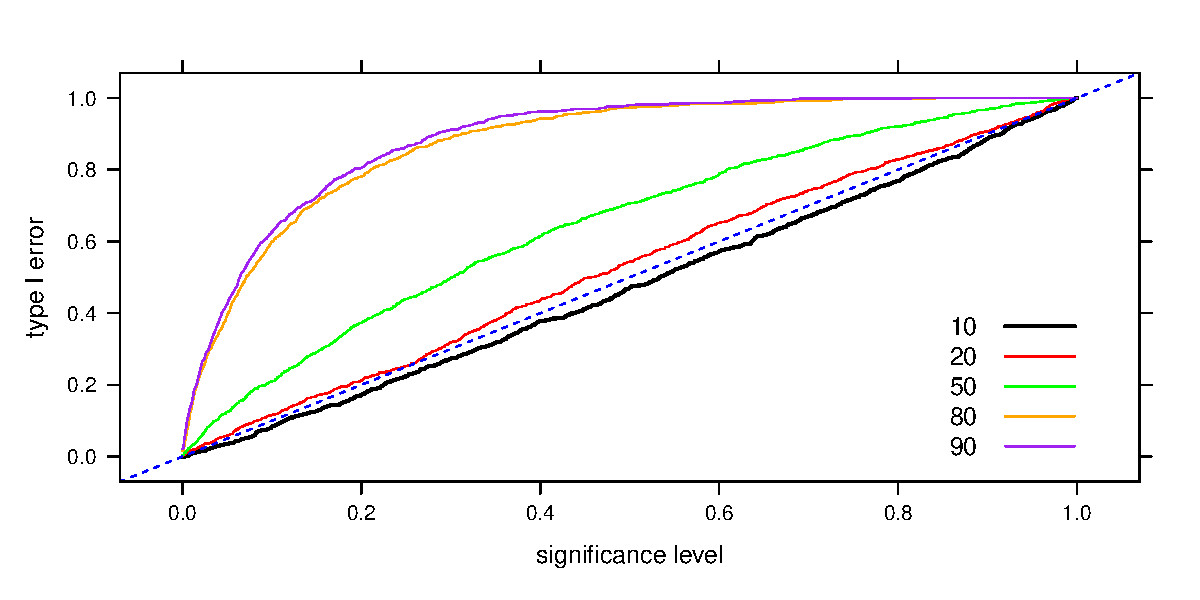
\includegraphics[width=.5\linewidth]{img/mcssa_comp_alphaI_ev.pdf}}\hfill
	\subfloat[Проекция на собственные векторы $\bfX\bfX^\rmT$]{\label{b}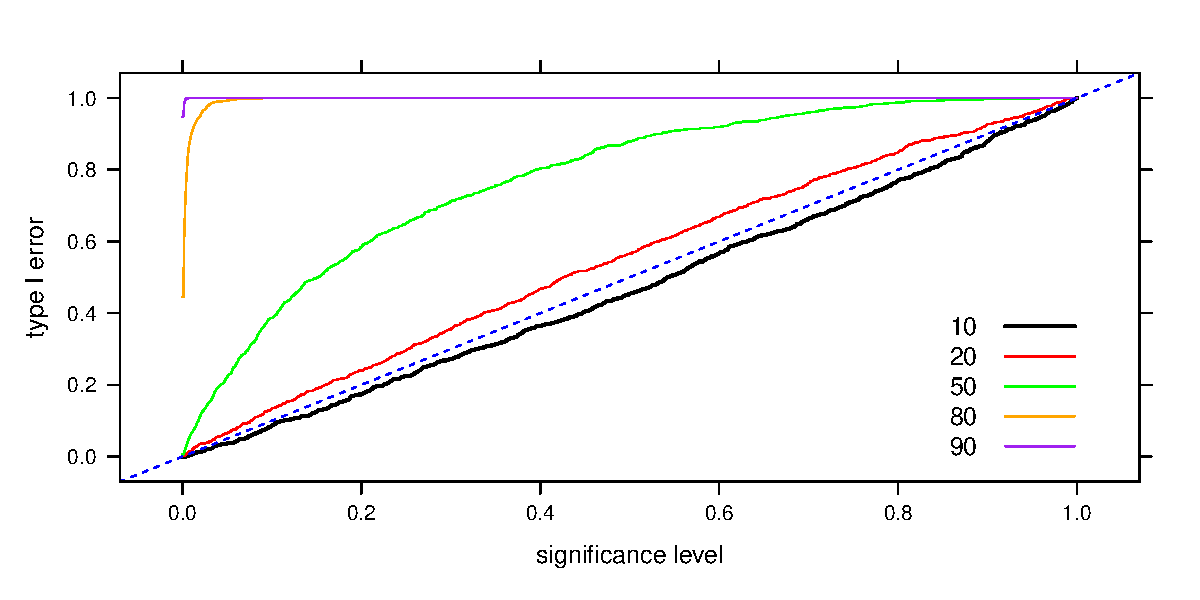
\includegraphics[width=.5\linewidth]{img/mcssa_comp_alphaI_ev_svd.pdf}}\par
	\subfloat[Проекция на косинусы]{\label{c}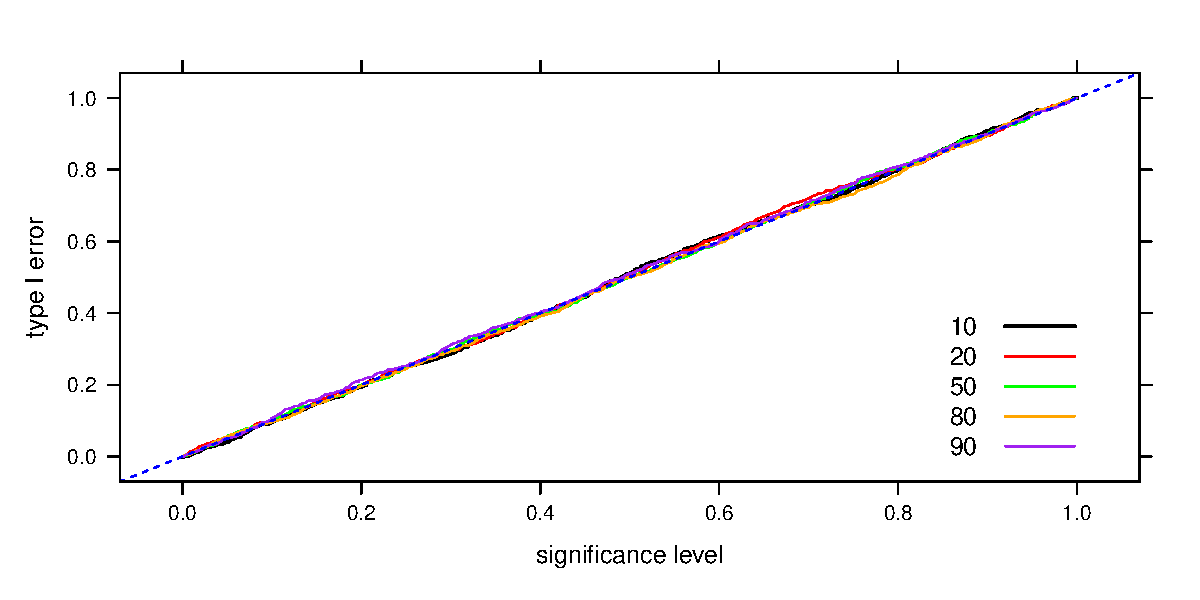
\includegraphics[width=.5\linewidth]{img/mcssa_comp_alphaI_cos.pdf}}
	\caption{Ошибка первого рода}
	\label{fig:mcssa_comp_alphaI}
\end{figure}

На рис.~\ref{fig:mcssa_comp_alphaI} изображены графики ошибок первого рода критериев <<ev>> и <<cos>> для рассматриваемых длин окна. Как видно по графикам, критерий <<ev>> радикальный для всех $L>10$, а <<cos>>, в свою очередь, является точным критерием для любой длины окна.

\begin{table}[h!]
	\centering
	\caption{Мощность поправленных критериев при уровне значимости $\alpha^*=0.1$}
	\label{tab:mcssa_comp_power}
	\begin{tabular}{c|c|c|c|c|c}
		$a=0$, $L\omega$~--- целые                      & $L=10$ & $L=20$ & $L=50$ & $L=80$ & $L=90$ \\
		\hline
		Проекция на собственные векторы $\bfT$          & 0.424  & 0.484  & 0.525  & 0.582  & 0.646  \\
		\hline
		Проекция на косинусы                            & 0.543  & 0.546  & 0.546  & 0.614  & 0.646  \\
		\hhline{======}
		$a=0$, $L\omega$~--- нецелые                    & $L=10$ & $L=20$ & $L=50$ & $L=80$ & $L=90$ \\
		\hline
		Проекция на собственные векторы $\bfT$          & 0.349  & 0.432  & 0.425  & 0.497  & 0.537  \\
		\hline
		Проекция на косинусы                            & 0.475  & 0.431  & 0.403  & 0.505  & 0.488  \\
		\hhline{======}
		$a\ne0$, $L\omega$~--- целые                    & $L=10$ & $L=20$ & $L=50$ & $L=80$ & $L=90$ \\
		\hline
		Проекция на собственные векторы $\bfX\bfX^\rmT$ & 0.329  & 0.303  & 0.307  & --     & --     \\
		\hline
		Проекция на косинусы                            & 0.480  & 0.347  & 0.163  & 0.228  & 0.299  \\
		\hhline{======}
		$a\ne0$, $L\omega$~--- нецелые                  & $L=10$ & $L=20$ & $L=50$ & $L=80$ & $L=90$ \\
		\hline
		Проекция на собственные векторы $\bfX\bfX^\rmT$ & 0.298  & 0.306  & 0.282  & --     & --     \\
		\hline
		Проекция на косинусы                            & 0.469  & 0.302  & 0.157  & 0.209  & 0.249  \\
	\end{tabular}
\end{table}

В таблице~\ref{tab:mcssa_comp_power} представлены значения мощности критериев после поправки, описанной в разделе~\ref{sect:correction} для рассмотренных $L$ при уровне значимости $\alpha^*=0.1$. Прочерки в таблице указывают на то, что критерий при данной длине окна слишком радикальный и построить поправку невозможно. Стоит отметить, что при $a\ne0$ ряд становится нестационарным, поэтому приходится использовать собственные векторы матрицы $\bfX\bfX^\rmT$, которые дают для больших $L$ слишком радикальный критерий и тем самым имеют потенциально меньшую мощность, чем при использовании собственных векторов матрицы $\bfT$.

По таблице видно, что оптимальной длиной окна при постоянной амплитуде сигнала ($a\ne0$) является $L=90$. В случае же модуляции оптимальной является $L=10$. Связано такое поведение мощности с тем, что при $a\ne0$ частота $\omega$, соответствующая сигналу, растекается по всему спектру частот и чем больше разрешение спектра (в данном случае $L$), тем сильнее это растекание. Если сравнивать по оптимальным $L$, то критерий <<cos>> дает наиболее мощный критерий в общем случае, когда модуляция непостоянная.

Учитывая большие вычислительные затраты критерия <<ev>>, и результат его численного сравнения с критерием <<cos>>, рекомендуется использовать косинусы в качестве проекционных векторов, поскольку критерий не является радикальным (следовательно не требует поправки, что заметно уменьшает трудоемкость MC-SSA) и по мощности не уступает, а в некоторых случаях даже превосходит вариант с векторами, порожденными исходным рядом.
% Далее будем рассматривать именно такой способ выбора векторов $W_k$ в алгоритме MC-SSA.

\section{Применение MC-SSA на реальных рядах}

В данном разделе рассмотрим проблемы, возникающие при применении MC-SSA на практике, а также их возможные решения.

\subsection{Ограниченность рассматриваемой модели шума}

В большинстве работ, посвященных MC-SSA, в качестве модели шума используется красный шум. Такая модель, хотя и описывает большой класс временных рядов, не является универсальной. Красный шум плохо описывает ряды, обладающие длинной памятью, то есть когда достаточно долго сохраняется зависимость от предыдущих значений.  

% \section{Процессы с длинной памятью}\label{sect:longmemory}

\begin{definition}\label{def:longmemory}
	Говорят, что стационарный процесс $\{Y_t\}$ обладает длинной памятью, если
	\[
		\sum_{h=0}^H|\gamma(h)|\to\infty,
	\]
	при $H\to\infty$. Иначе говорят, что $\{Y_t\}$ обладает короткой памятью:
	\[
		\sum_{h=0}^\infty|\gamma(h)|<\infty.
	\]
\end{definition}
Существуют и альтернативные определения процессов с длинной памятью, которые можно найти в~\cite[Раздел 3.1]{Palma2006}. Там же показано, что они согласованы с определением~\ref{def:longmemory}.
\begin{example}
	Процессом с короткой памятью является, например, стационарная модель $\mathrm{ARMA}(p, q)$, поскольку $|\gamma(h)|\leqslant CR^h$, где $C>0$ и $0<R<1$~\cite[Section 10.4]{BoxJenkins2016}.
\end{example}
Примером процесса с длинной памятью является модель $\textrm{ARFIMA}(p, d, q)$. Для ее определения введем понятие дробного дифференцирования $(1-L)^d$, где $L$~--- оператор сдвига. Для целых $d$ результат применения оператора интуитивен, например, для $d=1$ имеем $(1-L)Y_t=Y_t-Y_{t-1}$, для $d=2$~--- $(1-L)^2Y_t=Y_t-2Y_{t-1}+Y_{t-2}$, и так далее. Обобщим этот оператор для нецелых $d$ с помощью разложения в ряд Тейлора функции $(1-x)^d$ в нуле:
\[
	\begin{aligned}
		(1-x)^d & =1-dx-\frac{d(1-d)}{2}x^2-\frac{d(1-d)(2-d)}{3!}x^3-\ldots             \\
		        & =\sum_{j=0}^\infty \pi_j(d)x^j=\sum_{j=0}^\infty\binom{d}{j}(-1)^jx^j,
	\end{aligned}
\]
где $\binom{d}{j}$~--- обобщенный биномиальный коэффициент. Коэффициенты $\pi_j(d)$ удовлетворяют соотношению
\begin{equation}\label{eq:pi_j}
	\pi_j(d)=(-1)^j\binom{d}{j}=\frac{j-1-d}{j}\pi_{j-1}(d)=\frac{\Gamma(j-d)}{\Gamma(j+1)\Gamma(-d)},
\end{equation}
где $\Gamma(x)$~--- гамма функция. Заметим, что второе равенство в формуле~\eqref{eq:pi_j} верно для любых $d$, третье же верно только для $d\not\in\bbN\cup\{0\}$, поскольку гамма функция не определена для неположительных целых чисел.
\begin{definition}\label{def:arfima}
	Пусть процесс $\{Y_t\}$ определен соотношением
	\[
		\begin{aligned}
			Y_t=(1-L)^{-d}X_t=\sum_{k=0}^\infty \pi_k(-d)X_{t-k}
		\end{aligned},\quad d<1/2,
	\]
	где $\pi_k(-d)$ из формулы~\eqref{eq:pi_j}, $\{X_t\}$~--- стационарная и обратимая модель $\mathrm{ARMA}(p, d)$. Процесс $\{Y_t\}$ называют дробно интегрированной моделью $\mathrm{ARMA}$ или $\textrm{ARFIMA}(p, d, q)$.
\end{definition}
\begin{proposition}\label{prop1}
	Процесс $\{Y_t\}$ из определения~\ref{def:arfima} является стационарным процессом с нулевым средним. Его спектральная плотность определяется выражением
	\begin{equation}\label{eq:spec_long}
		\begin{aligned}
			f_Y(\omega) & =4^{-d}\sin^{-2d}\left(\pi\omega\right)f_X(\omega)                                                                                                      \\
			            & =4^{-d}\sin^{-2d}\left(\pi\omega\right)\sigma^2\frac{\left|\Theta(e^{-2\pi \omega\im})\right|^2}{\left|\Phi(e^{-2\pi\omega\im})\right|^2},\quad\omega>0 \\
			            & \sim\omega^{-2d}\sigma^2\frac{|\Theta(1)|^2}{|\Phi(1)|^2},\quad \omega\to0,
		\end{aligned}
	\end{equation}
	где $\Phi(L)$, $\Theta(L)$~--- характеристические полиномы процесса $\{X_t\}$.
\end{proposition}
\begin{proof}
	См.~\cite[Proposition 6.1]{Hassler2018}.
\end{proof}
\begin{remark}
	Из формулы~\eqref{eq:spec_long} видно, что монотонность спектральной плотности процесса $\{Y_t\}$ зависит от поведения спектральной плотности процесса $\{X_t\}$.
\end{remark}
\begin{corollary}\label{corollary1}
	В условиях предложения~\ref{prop1} при $0<d<1/2$
	\[
		\gamma(h)\sim C_{\gamma,d}h^{2d-1},\quad h\to\infty,
	\]
	где
	\[
		C_{\gamma,d}=\sigma^2 \frac{|\Theta(1)|^2}{|\Phi(1)|^2} \frac{\Gamma(1-2d)}{\Gamma(d)\Gamma(1-d)}.
	\]
\end{corollary}
\begin{proof}
	См.~\cite[Corollary 6.1]{Hassler2018}.
\end{proof}
\begin{remark}
	Из следствия~\ref{corollary1} сразу следует, что $\textrm{ARFIMA}(p, d, q)$ с $d\in(0, 1/2)$ обладает длинной памятью.
\end{remark}

\subsubsection{Сравнение MC-SSA по мощности при разных моделях шума}

Пусть $\bm \xi$~--- красный шум, а $\bm \eta$~--- модель $\textrm{ARFIMA}(0, d, 0)$. Будем считать дисперсию белого шума одинаковой для обоих процессов и равной $\sigma^2$. Дисперсии $\bm\xi$ и $\bm\eta$ соответственно равны
\[
	\mathsf{D}\bm\xi = \frac{\sigma^2}{1 - \phi^2}, \quad \mathsf{D}\bm\eta = \sigma^2\frac{\Gamma(1 - 2d)}{\Gamma(1-d)^2}.
\]
Тогда дисперсии процессов равны тогда и только тогда, когда
\[
	\phi=\pm\sqrt{1-\frac{\Gamma(1-d)^2}{\Gamma(1-2d)}}.
\]

\begin{figure}[h]
	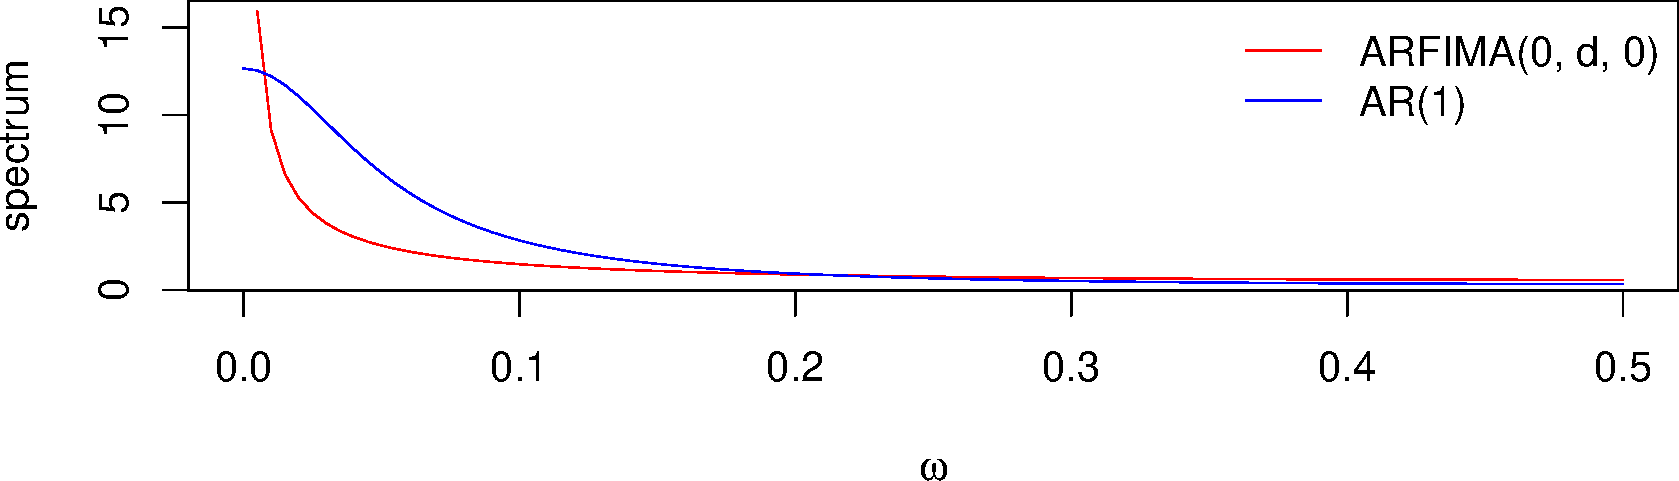
\includegraphics[width=\textwidth]{img/spectrum.pdf}
	\caption{Спектральная плотность процессов с одинаковой дисперсией}
	\label{fig:spectrum}
\end{figure}

Пусть $d=0.4$. Тогда при $\phi\approx0.719$ процессы $\bm\xi$ и $\bm\eta$ имеют одинаковую дисперсию. На рис.~\ref{fig:spectrum} изображены спектральные плотности процессов. На нем видно, что процесс $\bm\eta$ имеет меньшее значение плотности для всех значений $\omega\in(0, 0.2)$, за исключением близких к нулю.

Предполагается, что если рассмотреть в качестве альтернативы сигнал с частотой $\omega:f_{\bm\eta}(\omega) < f_{\bm\xi}(\omega)$, то мощность критерия MC-SSA против этой альтернативы при модели шума $\bm\eta$ больше, чем при модели шума $\bm\xi$. Убедимся в этом. Пусть длина ряда $N=100$, $\sigma^2=1$ и
\[
	\tS = \{A\cos(2 \pi n \omega)\}_{n=1}^N,\quad A=1,\ \omega=0.075.
\]

\begin{figure}[h]
	\begin{subfigure}{\textwidth}
		
\includegraphics[width=\textwidth]{img/alphaI_comp.pdf}
		\caption{Ошибка первого рода}
		\label{fig:ar1_vs_fi_alphaI}
	\end{subfigure}
	\begin{subfigure}{\textwidth}
		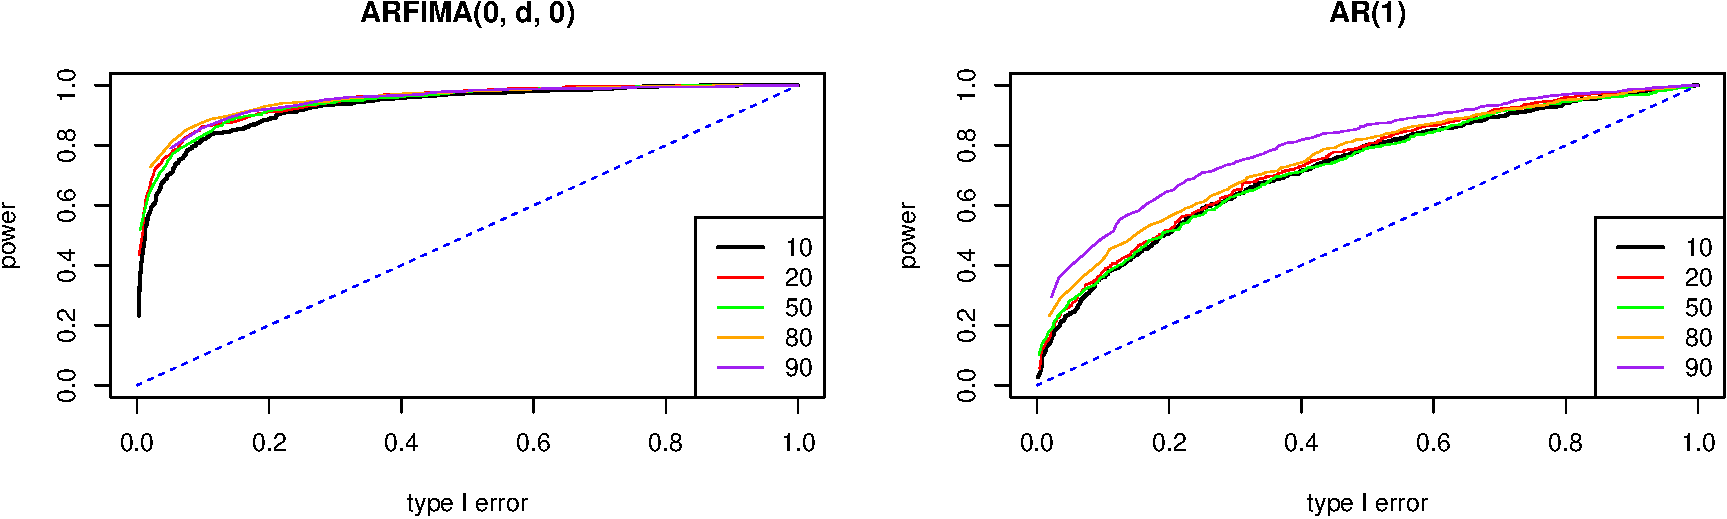
\includegraphics[width=\textwidth]{img/roc_comp.pdf}
		\caption{ROC-кривая}
		\label{fig:ar1_vs_fi_roc}
	\end{subfigure}
	\caption{Сравнение критерия MC-SSA при разных моделях шума}
	\label{fig:ar1_vs_fi}
\end{figure}

На рис.~\ref{fig:ar1_vs_fi_alphaI} изображены графики ошибок первого рода критериев MC-SSA для разных длин окна $L$. По ним видно, что рассматриваемые критерии являются радикальными, поэтому сравнивать их по мощности будем с помощью ROC-кривых, которые являются графиками мощности критериев, к которым была применена поправка из раздела~\ref{sect:correction}. По рис.~\ref{fig:ar1_vs_fi_roc} видно, что, действительно, мощность критерия против данной альтернативы при модели шума $\textrm{ARFIMA}(0, d, 0)$ больше, чем при модели шума $\textrm{AR}(1)$ с такой же дисперсией.

\subsection{Оценка параметров}

До сих пор предполагалось, что параметры шума $\bm\xi$ известны. В реальности параметры шума $\bm\xi$ неизвестны и их нужно оценивать. Тогда перед алгоритмом~\ref{alg:multiple_mc-ssa} необходимо оценить параметры модели $\bm\xi$ по исходному ряду. В данном разделе будем предполагать, что $\bm\xi$~--- модель ARFIMA($p$, $d$, $q$).

Пусть $\xi_t=(1-L)^{-d}\eta_t$, где $d<1/2$, $\bm\eta$~--- модель ARMA($p$, $q$) с белым гауссовским шумом $\bm\varepsilon$. Процесс $\bm\eta$ определяется следующим вектором параметров:
\[
\bm\psi=(\phi_1,\ldots,\phi_p,\theta_1,\ldots,\theta_q)^\rmT.
\]
Поставим задачу оценить параметры $\bm\varphi^\rmT=\left(d, \bm\psi^\rmT\right)$ и $\sigma^2$. Обозначим за $\bm{Y}=(Y_1,\ldots, Y_N)$ реализацию процесса $\bm\xi$ длины $N$.

\subsubsection{Maximum likelihood estimation (MLE)}

Поскольку $\bm\varepsilon$~--- гауссовский белый шум, вектор
\[
	\bm{Y} \sim \mathcal{N}(\bm0, \bm\Sigma_N),
\]
где $\bm\Sigma_N=(\gamma(|i-j|))_{i,j=1}^N$~--- ковариационная матрица вектора $\bm Y$. Совместная плотность распределения равна
\[
	(2\pi)^{-N/2} \left| \bm\Sigma_N \right|^{-1/2} \exp\left\{-\frac12 \bm{Y}^\rmT \bm\Sigma_N^{-1} \bm{Y}\right\}.
\]
Рассмотрим логарифм функции правдоподобия. Отбрасывая аддитивные константы, получаем
\[
	\ell(\bm\varphi, \sigma^2)=-\frac12 \ln\left|\bm{\Sigma}_N\right| - \frac12 \bm{Y}^\rmT \bm\Sigma_N^{-1} \bm{Y}.
\]
Положим $\bm\Gamma_n=\bm\Sigma_N / \sigma^2$ и, максимизируя $\ell$ по $\sigma^2$, получаем
\begin{equation}\label{eq:mle_objective}
	\ell_c(\bm\varphi)=-\frac{N}{2}\ln\left(S(\bm\varphi) / N\right) - \frac{1}{2}\ln g_N(\bm\varphi),
\end{equation}
где $S(\bm\varphi)=\bm Y^\rmT \bm\Gamma_N \bm Y$, $g_N(\bm\varphi)=\left|\bm\Gamma_N\right|$.
Тогда
\[
	\widehat{\bm\varphi}_\mathrm{ML}=\operatorname*{argmax}\limits_{\bm\varphi}\ell_c(\bm\varphi),\quad \widehat\sigma^2_\mathrm{ML} = S(\widehat{\bm\varphi}_\mathrm{ML}).
\]

\begin{remark}
	В случае ненулевого матожидания $\mathsf{E}\bm\xi=\mu$, для получения $\widehat{\bm\varphi}_\mathrm{ML}$ и $\widehat\sigma^2_\mathrm{ML}$ вместо $\bm Y$ рассматривается $\bm Z=\bm Y-\mu$. В случае неизвестного $\mu$ используется его состоятельная оценка $\overline{\bm{Y}}$.
\end{remark}
\begin{remark}
	Для вычисления $\ell_c$ можно использовать алгоритм Левинсона-Дурбина, имеющий временную трудоемкость $O(N^2)$~\cite{McLeod2007}.
\end{remark}

\subsubsection{Whittle estimation}\label{sect:whittle}

Метод максимального правдоподобия обладает двумя недостатками. Во-первых, неизвестное среднее вносит дополнительную неточность в оценку параметров. Во-вторых, существует проблема вычислительной сложности метода при больших $N$.

Обе эти проблемы можно решить, используя оценку Уиттла (Whittle): вместо логарифма функции правдоподобия рассматривается ее оценка (с точностью до константы)~\cite{Whittle1953}. Пусть $f_{\bm\xi}(\omega; \bm\varphi, \sigma^2)$~--- спектральная плотность $\bm\xi$, $I(\omega)$~--- периодограмма $\bm Y$, тогда
\begin{equation}\label{eq:whittle_loglik}
	\ell_W(\bm\varphi, \sigma^2)=-\frac1m\sum_{j=1}^m\left(\ln f_{\bm\xi}(\omega_j; \bm\varphi, \sigma^2) + \frac{I(\omega_j)}{f_{\bm\xi}(\omega_j; \bm\varphi, \sigma^2)}\right),
\end{equation}
где $m=\lfloor(N-1)/2\rfloor$, $\omega_j = j / N$, $j=1,2,\ldots,m$. Заметим, что $f_{\bm\xi}(\omega; \bm\varphi, \sigma^2)=\sigma^2 g_{\bm\xi}(\omega; \bm\varphi)$. Тогда, максимизируя $\ell_W$ по $\sigma^2$, получаем
\[
	\widehat{\bm\varphi}_W = \operatorname*{argmax}_{\bm\varphi}Q(\bm\varphi),\quad \widehat\sigma_W^2=\frac1m \sum_{j=1}^m\frac{I(\omega_j)}{g_{\bm\xi}(\omega_j; \widehat{\bm\varphi}_W)},
\]
где
\[
	Q(\bm\varphi)=-\ln\frac1m \sum_{j=1}^m\frac{I(\omega_j)}{g_{\bm\xi}(\omega_j; \bm\varphi)} - \frac1m \sum_{j=1}^m\ln g_{\bm\xi}(\omega_j; \bm\varphi).
\]
\begin{remark}
	Такой метод оценки параметров можно использовать при неизвестном среднем, поскольку при ее вычислении не используется значение периодограммы в нуле.
\end{remark}
\begin{remark}
	Периодограмму временного ряда можно вычислить за $O(N\log N)$ с помощью быстрого преобразования Фурье, что делает этот метод значительно быстрее MLE для больших $N$.
\end{remark}

\subsubsection{Численное сравнение методов оценки параметров}\label{sect:est_param}

Сравним качество оценок параметров следующих моделей:
\begin{enumerate}
	\item $d=q=0$, $p=1$~--- модель $\textrm{AR}(1)$;
	\item $p=q=0$~--- модель $\textrm{ARFIMA}(0, d, 0)$.
	\item $p=1$, $q=0$~--- модель $\textrm{ARFIMA}(1, d, 0)$.
\end{enumerate}
Для оценки параметров этих моделей на языке $\mathsf{R}$ были реализованы функции \textsf{arfima\_mle} и \textsf{arfima\_whittle}, которые соответствуют методам MLE и Whittle соответственно. Для реализации MLE были использованы функции \textsf{tacvfARFIMA} из пакета \textsf{arfima}~\cite{Veenstra2012} и \textsf{DLLoglikelihood} из пакета \textsf{ltsa}~\cite{McLeod2007}, вычисляющие автоковариационную функцию модели ARFIMA и функцию $\ell_c$~\eqref{eq:mle_objective} соответственно.

Помимо функций \textsf{arfima\_mle} и \textsf{arfima\_whittle}, будем использовать:
\begin{enumerate}
	\item Функцию \textsf{arima} из пакета \textsf{stats}, соответствующую MLE модели ARMA;
	\item Функцию \textsf{fracdiff} из пакета \textsf{fracdiff}~\cite{fracdiff}, соответствующую аппроксимации MLE модели ARFIMA, описанной в работе~\cite{Haslett1989} (обозначим ее за H\&R).
\end{enumerate}
\begin{remark}
	Помимо вышеперечисленных функций, в пакете \textsf{arfima} есть функция \textsf{arfima}, которая вычисляет MLE модели ARFIMA. Но данная реализация MLE в некоторых случаях дает оценки хуже, чем \textsf{arfima\_mle}. Сравнение оценок обоих реализаций можно найти в разделе~\ref{sect:mle_comparison}.
\end{remark}
Поскольку для реальных временных рядов матожидание $\mu$ неизвестно, будем рассматривать MLE с известным средним и с его оценкой~--- выборочным средним (будем обозначать их $\mathrm{MLE}(\mu)$ и $\mathrm{MLE}(\bar x)$ соответственно). Не умаляя общности, пусть $\mu=0$.

\begin{figure}[h]
	\centering
	\begin{subfigure}{\textwidth}
		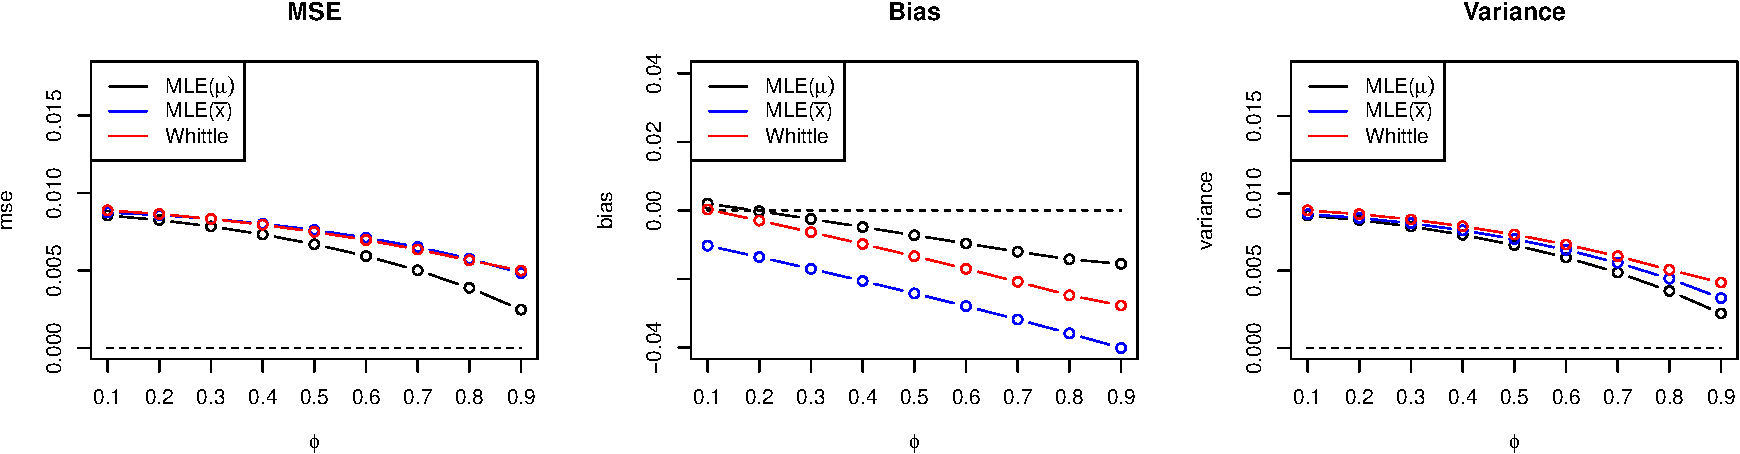
\includegraphics[width=\textwidth]{img/ar1_est_N100.pdf}
		\caption{$N=100$}
	\end{subfigure}
	\begin{subfigure}{\textwidth}
		
\includegraphics[width=\textwidth]{img/ar1_est_N1000.pdf}
		\caption{$N=1000$}
	\end{subfigure}
	\caption{Среднеквадратичное отклонение, смещение и дисперсия оценок параметра $\phi$ модели $\textrm{AR}(1)$ ($500$ повторений)}
	\label{fig:ar1_est}
\end{figure}
\begin{figure}[h]
	\centering
	\begin{subfigure}{\textwidth}
		
\includegraphics[width=\textwidth]{img/fi_est_N100.pdf}
		\caption{$N=100$}
	\end{subfigure}
	\begin{subfigure}{\textwidth}
		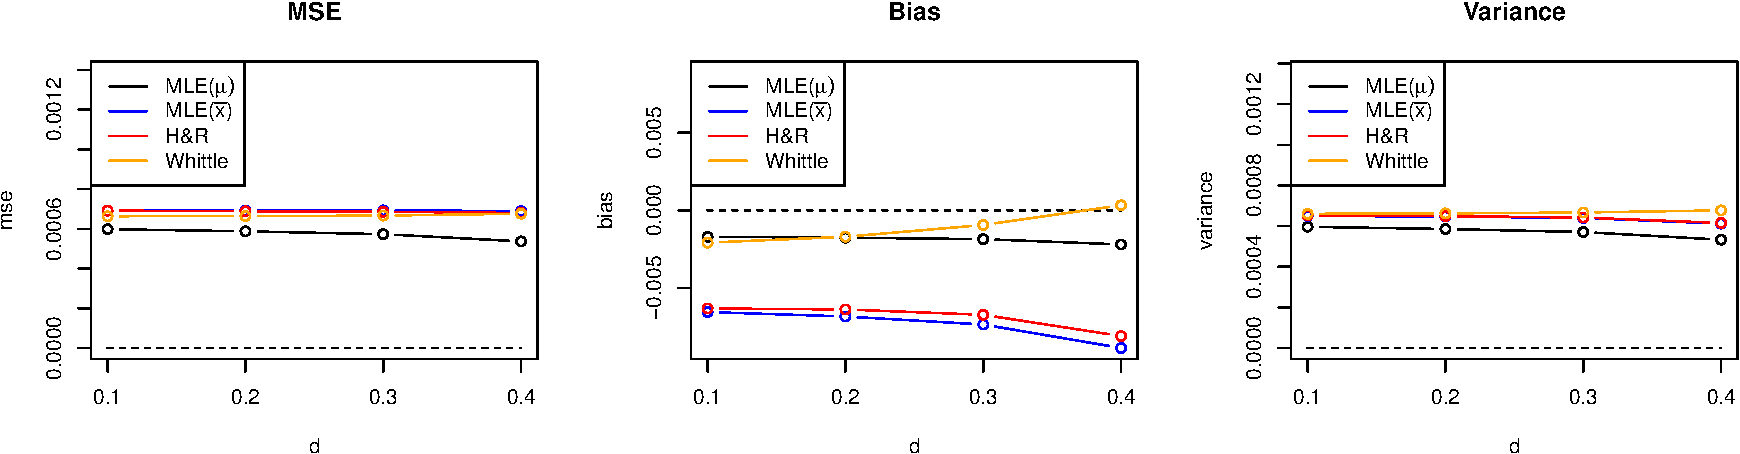
\includegraphics[width=\textwidth]{img/fi_est_N1000.pdf}
		\caption{$N=1000$}
	\end{subfigure}
	\caption{Среднеквадратичное отклонение, смещение и дисперсия оценок параметра $d$ модели $\textrm{ARFIMA}(0, d, 0)$ ($500$ повторений)}
	\label{fig:fi_est}
\end{figure}

На рис.~\ref{fig:ar1_est} и~\ref{fig:fi_est} изображены среднеквадратичное отклонение, смещение и дисперсия оценок параметров $\phi$ и $d$ моделей $\textrm{AR}(1)$ и $\textrm{ARFIMA}(0, d, 0)$. Отметим, что все оценки имеют в большинстве своем отрицательное смещение и отличаются между собой в основном степенью смещения. Как и ожидалось, оценка параметров методом максимального правдоподобия с известным средним дает оценку с наименьшим $\mathsf{MSE}$. С другой стороны, если использовать вместо известного среднего выборочное среднее, оценки становятся сильно смещенными. Whittle же, в свою очередь, дает менее смещенную оценку, чем $\mathrm{MLE}(\bar x)$, а в случае оценки $d$ имеет смещение даже меньше, чем у $\textrm{MLE}(\mu)$. Однако оценки Whittle обладают наибольшей дисперсией среди всех рассмотренных методов, но разница не такая значительная, как в случае смещения.

\begin{sidewaystable}[h!]
	\centering
	\caption{Смещение и среднеквадратичное отклонение оценок параметров $d$ и $\phi$ модели $\textrm{ARFIMA}(1, d, 0)$ ($N=100$, $500$ повторений)}
	\label{tab:arfi_est_n100}
	\scalebox{0.9}{
		\begin{tabular}{m{1cm}m{1cm}ccccccccm{0.2cm}cccccccc}
			\hline
			    &        & \multicolumn{8}{c}{$\mathsf{MSE}$}      &                                            & \multicolumn{8}{c}{$\mathsf{Bias}$}                                                                                                                                                                                                                                                                                                                                                                                                              \\
			\cline{3-10} \cline{12-19}
			    &        & \multicolumn{2}{c}{$\mathrm{MLE}(\mu)$} & \multicolumn{2}{c}{$\mathrm{MLE}(\bar x)$} & \multicolumn{2}{c}{H\&R}            & \multicolumn{2}{c}{Whittle} &                         & \multicolumn{2}{c}{$\mathrm{MLE}(\mu)$} & \multicolumn{2}{c}{$\mathrm{MLE}(\bar x)$} & \multicolumn{2}{c}{H\&R} & \multicolumn{2}{c}{Whittle}                                                                                                                                                                                                      \\
			$d$ & $\phi$ & $\hat d$                                & $\hat\phi$                                 & $\hat d$                            & $\hat\phi$                  & $\hat d$                & $\hat\phi$                              & $\hat d$                                   & $\hat\phi$               &                             & $\hat d$                 & $\hat\phi$             & $\hat d$                 & $\hat\phi$ & $\hat d$                 & $\hat\phi$              & $\hat d$                 & $\hat\phi$             \\ \hline
			0.1 & 0.1    & 0.049                                   & 0.056                                      & 0.119                               & 0.114                       & \textcolor{blue}{0.009} & \textcolor{red}{0.018}                  & 0.069                                      & 0.067                    &                             & -0.077                   & 0.066                  & -0.229                   & 0.199      & \textcolor{blue}{-0.054} & \textcolor{red}{0.035}  & -0.086                   & 0.068                  \\
			0.2 & 0.1    & 0.047                                   & 0.055                                      & 0.151                               & 0.141                       & \textcolor{blue}{0.025} & \textcolor{red}{0.032}                  & 0.077                                      & 0.073                    &                             & \textcolor{blue}{-0.078} & \textcolor{red}{0.067} & -0.265                   & 0.232      & -0.119                   & 0.099                   & -0.094                   & 0.074                  \\
			0.3 & 0.1    & \textcolor{blue}{0.041}                 & \textcolor{red}{0.049}                     & 0.183                               & 0.165                       & 0.049                   & 0.055                                   & 0.084                                      & 0.081                    &                             & \textcolor{blue}{-0.076} & \textcolor{red}{0.066} & -0.301                   & 0.266      & -0.179                   & 0.161                   & -0.109                   & 0.09                   \\
			0.4 & 0.1    & \textcolor{blue}{0.029}                 & \textcolor{red}{0.038}                     & 0.211                               & 0.187                       & 0.081                   & 0.089                                   & 0.179                                      & 0.194                    &                             & \textcolor{blue}{-0.072} & \textcolor{red}{0.065} & -0.34                    & 0.305      & -0.243                   & 0.23                    & -0.26                    & 0.241                  \\
			\hline
			0.1 & 0.5    & 0.045                                   & 0.041                                      & 0.086                               & 0.053                       & \textcolor{blue}{0.010} & \textcolor{red}{0.015}                  & 0.057                                      & 0.054                    &                             & -0.071                   & 0.034                  & -0.222                   & 0.151      & -0.07                    & 0.034                   & \textcolor{blue}{-0.066} & \textcolor{red}{0.024} \\
			0.2 & 0.5    & 0.042                                   & 0.038                                      & 0.092                               & 0.055                       & \textcolor{blue}{0.031} & \textcolor{red}{0.025}                  & 0.074                                      & 0.058                    &                             & \textcolor{blue}{-0.081} & \textcolor{red}{0.046} & -0.244                   & 0.171      & -0.154                   & 0.108                   & -0.153                   & 0.107                  \\
			0.3 & 0.5    & \textcolor{blue}{0.040}                 & \textcolor{red}{0.036}                     & 0.1                                 & 0.059                       & 0.063                   & 0.043                                   & 0.098                                      & 0.062                    &                             & \textcolor{blue}{-0.093} & \textcolor{red}{0.060} & -0.267                   & 0.192      & -0.232                   & 0.174                   & -0.209                   & 0.161                  \\
			0.4 & 0.5    & \textcolor{blue}{0.037}                 & \textcolor{red}{0.033}                     & 0.115                               & 0.067                       & 0.104                   & 0.065                                   & 0.104                                      & 0.066                    &                             & \textcolor{blue}{-0.103} & \textcolor{red}{0.073} & -0.304                   & 0.226      & -0.306                   & 0.235                   & -0.228                   & 0.177                  \\
			\hline
			0.1 & 0.9    & 0.029                                   & 0.029                                      & 0.014                               & 0.01                        & \textcolor{blue}{0.007} & \textcolor{red}{0.007}                  & 0.034                                      & 0.025                    &                             & 0.075                    & -0.089                 & 0.01                     & -0.049     & \textcolor{blue}{0.001}  & \textcolor{red}{-0.043} & 0.049                    & -0.069                 \\
			0.2 & 0.9    & 0.019                                   & 0.018                                      & 0.011                               & 0.006                       & \textcolor{blue}{0.009} & \textcolor{red}{0.004}                  & 0.026                                      & 0.019                    &                             & 0.046                    & -0.065                 & \textcolor{blue}{-0.011} & -0.035     & -0.037                   & \textcolor{red}{-0.026} & 0.02                     & -0.056                 \\
			0.3 & 0.9    & 0.012                                   & 0.01                                       & \textcolor{blue}{0.009}             & 0.004                       & 0.014                   & \textcolor{red}{0.003}                  & 0.022                                      & 0.015                    &                             & \textcolor{blue}{0.016}  & -0.043                 & -0.033                   & -0.023     & -0.076                   & \textcolor{red}{-0.011} & -0.024                   & -0.039                 \\
			0.4 & 0.9    & \textcolor{blue}{0.008}                 & 0.006                                      & 0.009                               & \textcolor{red}{0.002}      & 0.025                   & \textcolor{red}{0.002}                  & 0.028                                      & 0.01                     &                             & \textcolor{blue}{-0.016} & -0.024                 & -0.061                   & -0.008     & -0.121                   & \textcolor{red}{0.003}  & -0.095                   & -0.016                 \\ \hline
		\end{tabular}
	}
\end{sidewaystable}

\begin{sidewaystable}[h!]
	\centering
	\caption{Смещение и среднеквадратичное отклонение оценок параметров $d$ и $\phi$ модели $\textrm{ARFIMA}(1, d, 0)$ ($N=1000$, $500$ повторений)}
	\label{tab:arfi_est_n1000}
	\scalebox{0.9}{
		\begin{tabular}{m{1cm}m{1cm}ccccccccm{0.2cm}cccccccc}
			\hline
			    &        & \multicolumn{8}{c}{$\mathsf{MSE} \cdot 100$} &                                            & \multicolumn{8}{c}{$\mathsf{Bias} \cdot 100$}                                                                                                                                                                                                                                                                                                                                                                                                           \\
			\cline{3-10} \cline{12-19}
			    &        & \multicolumn{2}{c}{$\mathrm{MLE}(\mu)$}      & \multicolumn{2}{c}{$\mathrm{MLE}(\bar x)$} & \multicolumn{2}{c}{H\&R}                      & \multicolumn{2}{c}{Whittle} &                         & \multicolumn{2}{c}{$\mathrm{MLE}(\mu)$} & \multicolumn{2}{c}{$\mathrm{MLE}(\bar x)$} & \multicolumn{2}{c}{H\&R} & \multicolumn{2}{c}{Whittle}                                                                                                                                                                                                   \\
			$d$ & $\phi$ & $\hat d$                                     & $\hat\phi$                                 & $\hat d$                                      & $\hat\phi$                  & $\hat d$                & $\hat\phi$                              & $\hat d$                                   & $\hat\phi$               &                             & $\hat d$                 & $\hat\phi$             & $\hat d$                 & $\hat\phi$             & $\hat d$ & $\hat\phi$              & $\hat d$                 & $\hat\phi$              \\ \hline
			0.1 & 0.1    & \textcolor{blue}{0.186}                      & \textcolor{red}{0.290}                     & 0.27                                          & 0.37                        & 0.224                   & 0.317                                   & 0.232                                      & 0.33                     &                             & \textcolor{blue}{-0.581} & \textcolor{red}{0.448} & -1.941                   & 1.732                  & -1.729   & 1.508                   & -0.687                   & 0.519                   \\
			0.2 & 0.1    & \textcolor{blue}{0.181}                      & \textcolor{red}{0.287}                     & 0.271                                         & 0.371                       & 0.267                   & 0.366                                   & 0.232                                      & 0.329                    &                             & \textcolor{blue}{-0.599} & \textcolor{red}{0.465} & -2.026                   & 1.824                  & -1.981   & 1.773                   & -0.615                   & 0.468                   \\
			0.3 & 0.1    & \textcolor{blue}{0.174}                      & \textcolor{red}{0.282}                     & 0.272                                         & 0.372                       & 0.268                   & 0.367                                   & 0.232                                      & 0.328                    &                             & -0.639                   & 0.505                  & -2.177                   & 1.987                  & -2.176   & 1.975                   & \textcolor{blue}{-0.476} & \textcolor{red}{0.372}  \\
			0.4 & 0.1    & \textcolor{blue}{0.156}                      & \textcolor{red}{0.267}                     & 0.272                                         & 0.373                       & 0.274                   & 0.371                                   & 0.232                                      & 0.325                    &                             & -0.795                   & 0.666                  & -2.606                   & 2.443                  & -2.725   & 2.542                   & \textcolor{blue}{-0.263} & \textcolor{blue}{0.233} \\
			\hline
			0.1 & 0.1    & 0.761                                        & 0.8                                        & 1.429                                         & 1.3                         & \textcolor{blue}{0.504} & \textcolor{red}{0.552}                  & 1.104                                      & 1.05                     &                             & \textcolor{blue}{-2.047} & \textcolor{red}{1.588} & -5.86                    & 5.102                  & -3.256   & 2.741                   & -2.555                   & 1.904                   \\
			0.2 & 0.1    & \textcolor{blue}{0.710}                      & \textcolor{red}{0.759}                     & 1.432                                         & 1.302                       & 0.978                   & 0.969                                   & 1.213                                      & 1.125                    &                             & \textcolor{blue}{-2.018} & \textcolor{red}{1.571} & -6.08                    & 5.337                  & -5.157   & 4.556                   & -2.721                   & 2.065                   \\
			0.3 & 0.1    & \textcolor{blue}{0.617}                      & \textcolor{red}{0.675}                     & 1.462                                         & 1.323                       & 1.246                   & 1.175                                   & 1.23                                       & 1.15                     &                             & \textcolor{blue}{-1.984} & \textcolor{red}{1.560} & -6.506                   & 5.78                   & -6.129   & 5.463                   & -2.578                   & 1.948                   \\
			0.4 & 0.1    & \textcolor{blue}{0.473}                      & \textcolor{red}{0.539}                     & 1.499                                         & 1.353                       & 1.507                   & 1.354                                   & 1.294                                      & 1.18                     &                             & \textcolor{blue}{-2.226} & \textcolor{red}{1.861} & -7.514                   & 6.838                  & -7.622   & 6.905                   & -2.695                   & 2.099                   \\
			\hline
			0.1 & 0.9    & 0.338                                        & 0.155                                      & 0.288                                         & 0.122                       & \textcolor{blue}{0.259} & \textcolor{red}{0.097}                  & 0.387                                      & 0.193                    &                             & 0.623                    & -0.774                 & \textcolor{blue}{-0.095} & -0.56                  & -0.176   & \textcolor{red}{-0.504} & 0.583                    & -0.92                   \\
			0.2 & 0.9    & 0.273                                        & 0.106                                      & \textcolor{blue}{0.233}                       & \textcolor{red}{0.077}      & 0.239                   & 0.077                                   & 0.326                                      & 0.128                    &                             & 0.42                     & -0.611                 & -0.388                   & -0.355                 & -0.627   & \textcolor{red}{-0.303} & \textcolor{blue}{0.041}  & -0.652                  \\
			0.3 & 0.9    & 0.241                                        & 0.093                                      & \textcolor{blue}{0.217}                       & \textcolor{red}{0.068}      & 0.268                   & 0.075                                   & 0.326                                      & 0.097                    &                             & \textcolor{blue}{0.287}  & -0.53                  & -0.667                   & -0.204                 & -1.395   & \textcolor{red}{-0.029} & -1.003                   & -0.285                  \\
			0.4 & 0.9    & \textcolor{blue}{0.173}                      & 0.067                                      & 0.182                                         & \textcolor{red}{0.051}      & 0.381                   & 0.076                                   & 0.545                                      & 0.09                     &                             & \textcolor{blue}{-0.129} & -0.295                 & -1.4                     & \textcolor{red}{0.178} & -2.602   & 0.359                   & -3.357                   & 0.389                   \\
			\hline
		\end{tabular}
	}
\end{sidewaystable}

В таблицах~\ref{tab:arfi_est_n100} и~\ref{tab:arfi_est_n1000} представлены значения среднеквадратичной ошибки и смещения оценок параметров $d$ и $\phi$ модели $\textrm{ARFIMA}(1, d)$. Заметим, что в оценках присутствует смещение, для $\phi=0.1$ и $\phi=0.5$ оценки $d$ имеют отрицательное смещение, а оценки $\phi$, наоборот, положительное. Также в таблицах синим цветом выделена лучшая по строке оценка $d$, а красным~--- лучшая оценка $\phi$. Видно, что в случае коротких рядов ($N=100$) метод H\&R в большинстве случаев дает оценки с наименьшим $\mathsf{MSE}$, однако наименьшее смещение имеют оценки $\mathrm{MLE}(\mu)$. В случае же длинных рядов ($N=1000$) наименьшую среднеквадратичную ошибку и смещение дает $\mathrm{MLE}(\mu)$. Отметим, что даже для длинных рядов оценки $\mathrm{MLE}(\bar x)$ имеют, в большинстве случаев, наибольшее смещение и $\mathsf{MSE}$. Оценки H\&R, хотя и дают наименьшее после $\mathrm{MLE}(\mu)$ $\mathsf{MSE}$, также сильно смещены. Оценки методом Whittle выглядят наиболее привлекательными, поскольку имеют наименьшее после $\mathrm{MLE}(\mu)$ смещение и имеют $\mathsf{MSE}$ меньше, чем $\mathrm{MLE}(\bar x)$.

Подведем итоги численного сравнения. Если для рассматриваемого ряда известно его матожидание $\mu$ (что, конечно, редкость на практике), наилучшим методом является $\mathrm{MLE}(\mu)$. Если же среднее неизвестно, для коротких рядов оценивать параметры моделей $\textrm{AR}(1)$ и $\textrm{ARFIMA}(0, d, 0)$ следует методом Whittle, а параметры модели $\textrm{ARFIMA}(1, d, 0)$~--- методом H\&R. В случае длинных рядов параметры рассматриваемых моделей следует оценивать методом Whittle.

% \begin{table}[h!]
% 	\centering
% 	\caption{Смещение и среднеквадратичное отклонение оценок параметра $\phi$ модели $\textrm{AR}(1)$ ($n=100$, $500$ повторений)}
% 	\begin{tabular}{m{1cm}cccm{0.5cm}ccc}
% 		\hline
% 		& \multicolumn{3}{c}{$\mathsf{bias}\cdot 100$} & & \multicolumn{3}{c}{$\mathsf{MSE}\cdot 100$} \\
% 		\cline{2-4} \cline{6-8}
% 		$\phi$ & $\mathrm{MLE}(\mu)$ & $\mathrm{MLE}(\bar x)$ & Whittle & & $\mathrm{MLE}(\mu)$ & $\mathrm{MLE}(\bar x)$ & Whittle \\ \hline
% 		0.1 & 0.197  & -1.029 &  0.025 & & 0.856 & 0.874 & 0.889\\
% 		0.2 & -0.023 & -1.362 & -0.298 & & 0.826 & 0.859 & 0.865\\
% 		0.3 & -0.252 & -1.707 & -0.635 & & 0.785 & 0.834 & 0.834\\
% 		0.4 & -0.487 & -2.061 & -0.981 & & 0.733 & 0.802 & 0.796\\
% 		0.5 & -0.725 & -2.423 & -1.337 & & 0.670 & 0.762 & 0.75\\
% 		0.6 & -0.965 & -2.796 & -1.704 & & 0.594 & 0.712 & 0.697\\
% 		0.7 & -1.205 & -3.183 & -2.084 & & 0.502 & 0.652 & 0.636\\
% 		0.8 & -1.427 & -3.59  & -2.478 & & 0.389 & 0.577 & 0.566\\
% 		0.9 & -1.560 & -4.016 & -2.777 & & 0.248 & 0.483 & 0.5\\
% 		\hline
% 	\end{tabular}
% \end{table}

\subsubsection{Сходимость оценок к истинным значениям}
Известно~\cite[Theorem 8.1]{Hassler2018}, что
\begin{equation}\label{eq:mle_distribution}
	\sqrt{n}(\widehat{\bm\varphi}_\mathrm{ML} - \bm\varphi_0)\overset{d}{\longrightarrow} \mathcal{N}(0, \mathcal{I}^{-1}(\bm{\varphi}_0)),
\end{equation}
где $\bm\varphi_0$~--- истинный вектор параметров, $\mathcal{I}(\bm\varphi)$~--- информационная матрица Фишера. Также известно~\cite[Proposition 8.3]{Hassler2018}, что вектор $\widehat{\bm\varphi}_W$ имеет такое же асимптотическое распределение, что и $\widehat{\bm\varphi}_\mathrm{ML}$.

Покажем, что методы $\mathrm{MLE}(\mu)$ и Whittle реализованы корректно, посмотрев на дисперсию оценок для $N=10000$. В таблице~\ref{tab:variance} представлены оценки дисперсий $\hat d$ и $\hat \phi$, в скобках указана теоретическая дисперсия. Как видим, для разных значений параметров значение дисперсий оценок близки к теоретическим.

\begin{table}[h]
	\centering
	\subfloat[$d=0.2$, $\varphi=0.1$]{
		\begin{tabular}{c|cc}
			Метод               & $n\mathsf{D} \hat d$ (1.83167) & $n\mathsf{D}\hat \phi$ (2.98284) \\
			\hline
			$\mathrm{MLE}(\mu)$ & 1.72733                        & 2.92604                          \\
			Whittle             & 1.78350                        & 2.94929                          \\
			\hline
		\end{tabular}
	}
	\subfloat[$d=0.4$, $\varphi=0.1$]{
		\begin{tabular}{c|cc}
			Метод               & $n\mathsf{D} \hat d$ (1.83167) & $n\mathsf{D}\hat \phi$ (2.98284) \\
			\hline
			$\mathrm{MLE}(\mu)$ & 1.69348                        & 2.90374                          \\
			Whittle             & 1.84265                        & 2.96828                          \\
			\hline
		\end{tabular}
	}\vspace{2em}
	\subfloat[$d=0.2$, $\varphi=0.5$]{
		\begin{tabular}{c|cc}
			Метод               & $n\mathsf{D} \hat d$ (4.91219) & $n\mathsf{D}\hat \phi$ (6.06018) \\
			\hline
			$\mathrm{MLE}(\mu)$ & 5.00869                        & 6.305                            \\
			Whittle             & 5.08405                        & 6.35985                          \\
			\hline
		\end{tabular}
	}
	\subfloat[$d=0.4$, $\varphi=0.5$]{
		\begin{tabular}{c|cc}
			Метод               & $n\mathsf{D} \hat d$ (4.91219) & $n\mathsf{D}\hat \phi$ (6.06018) \\
			\hline
			$\mathrm{MLE}(\mu)$ & 4.75975                        & 6.06711                          \\
			Whittle             & 5.28104                        & 6.4936                           \\
			\hline
		\end{tabular}
	}\vspace{2em}
	\subfloat[$d=0.2$, $\varphi=0.9$]{
		\begin{tabular}{c|cc}
			Метод               & $n \mathsf{D} \hat d$ (2.49203) & $n\mathsf{D}\hat \phi$ (0.77885) \\
			\hline
			$\mathrm{MLE}(\mu)$ & 2.42011                         & 0.78209                          \\
			Whittle             & 2.44394                         & 0.77549                          \\
			\hline
		\end{tabular}
	}
	\subfloat[$d=0.4$, $\varphi=0.9$]{
		\begin{tabular}{c|cc}
			Метод               & $n \mathsf{D} \hat d$ (2.49203) & $n\mathsf{D}\hat \phi$ (0.77885) \\
			\hline
			$\mathrm{MLE}(\mu)$ & 2.26718                         & 0.749318                         \\
			Whittle             & 2.57117                         & 0.77311                          \\
			\hline
		\end{tabular}
	}
	\caption{Дисперсия оценок $\hat d$ и $\hat \phi$, $n=10000$, $100$ повторений}
	\label{tab:variance}
\end{table}

\subsubsection{Искажение критерия MC-SSA при оценке параметров шума}\label{sect:mcssa_est_model}

В работе~\cite{Poteshkin2024} показано, что оценка параметров несильно искажает критерий, но делает его консервативнее. Для наглядности на рис.~\ref{fig:alphaI_true_est_ev} и~\ref{fig:alphaI_true_est_cos} изображены ошибки первого рода для примера из раздела~\ref{sect:mcssa_comp}, параметры оценивались с помощью метода Уиттла (см. раздел~\ref{sect:whittle}). Как видно из графиков, оценка параметров уменьшила радикальность критерия <<ev>> и сделала консервативным критерий <<cos>>.

\begin{figure}[!htbp]
	\centering
	\begin{subfigure}{0.45\linewidth}
		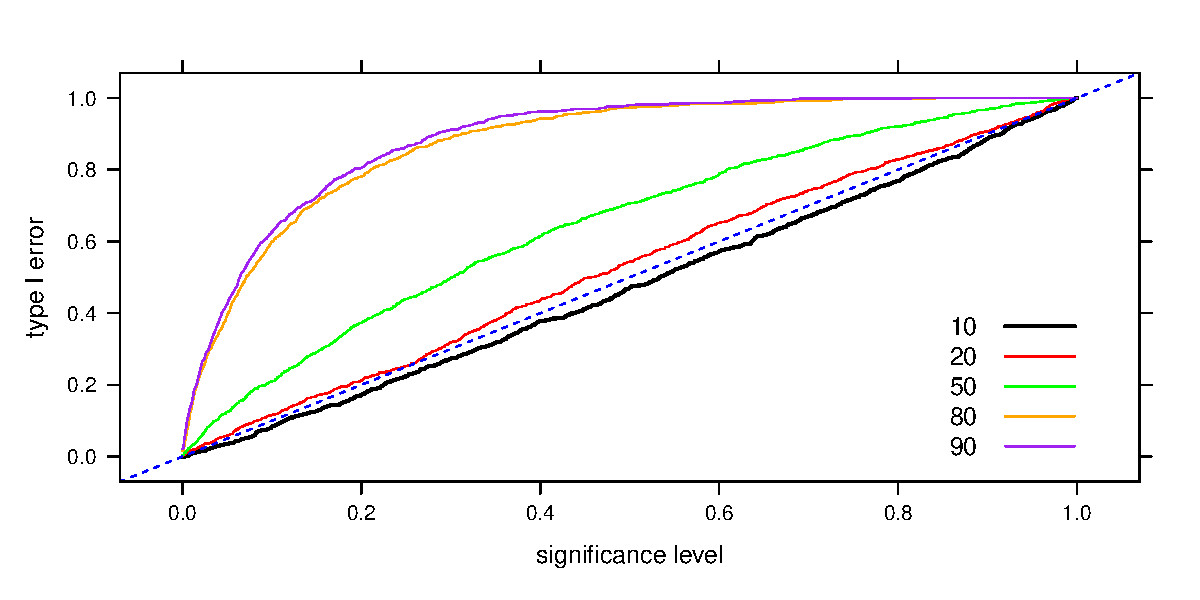
\includegraphics[width=\linewidth]{img/mcssa_comp_alphaI_ev.pdf}
		\caption{Истинные параметры шума}
	\end{subfigure}
	\begin{subfigure}{0.45\linewidth}
		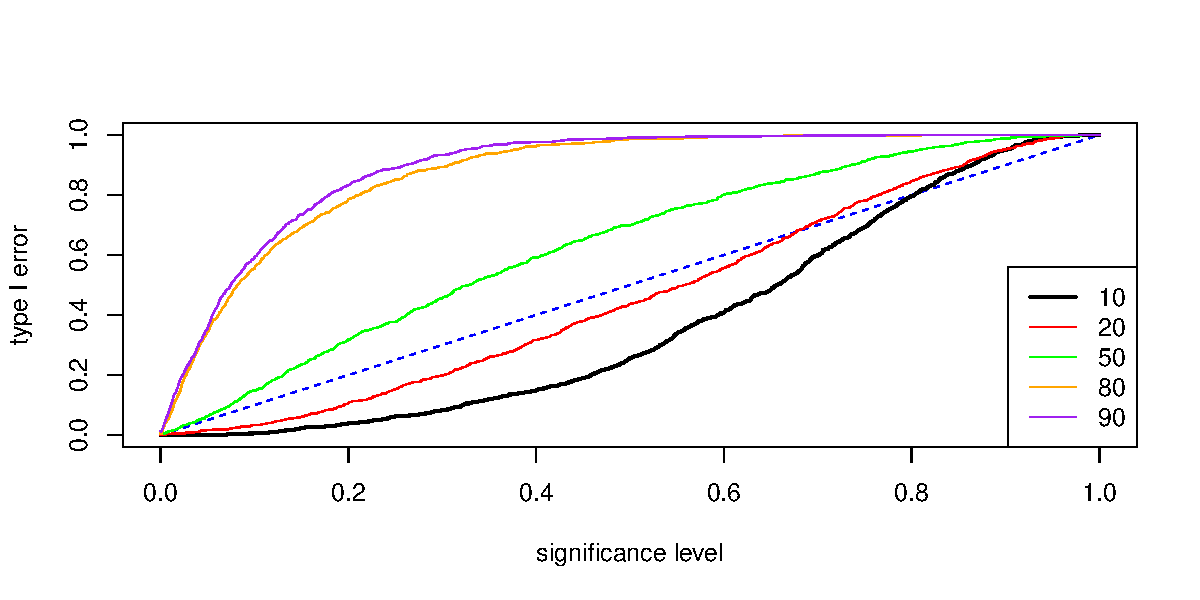
\includegraphics[width=\linewidth]{img/alphaI_ev_est.pdf}
		\caption{Оцененные параметры шума}
	\end{subfigure}
	\caption{Ошибка первого рода для разных длин окна (критерий <<ev>>)}
	\label{fig:alphaI_true_est_ev}
\end{figure}

\begin{figure}[!htbp]
	\centering
	\begin{subfigure}{0.45\linewidth}
		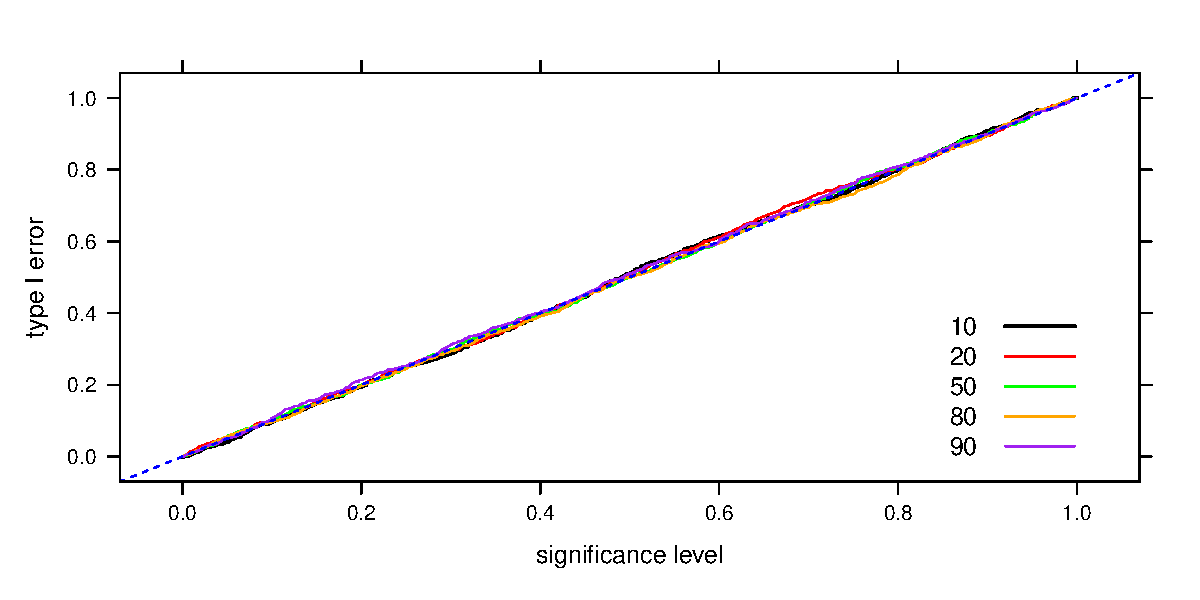
\includegraphics[width=\linewidth]{img/mcssa_comp_alphaI_cos.pdf}
		\caption{Истинные параметры шума}
	\end{subfigure}
	\begin{subfigure}{0.45\linewidth}
		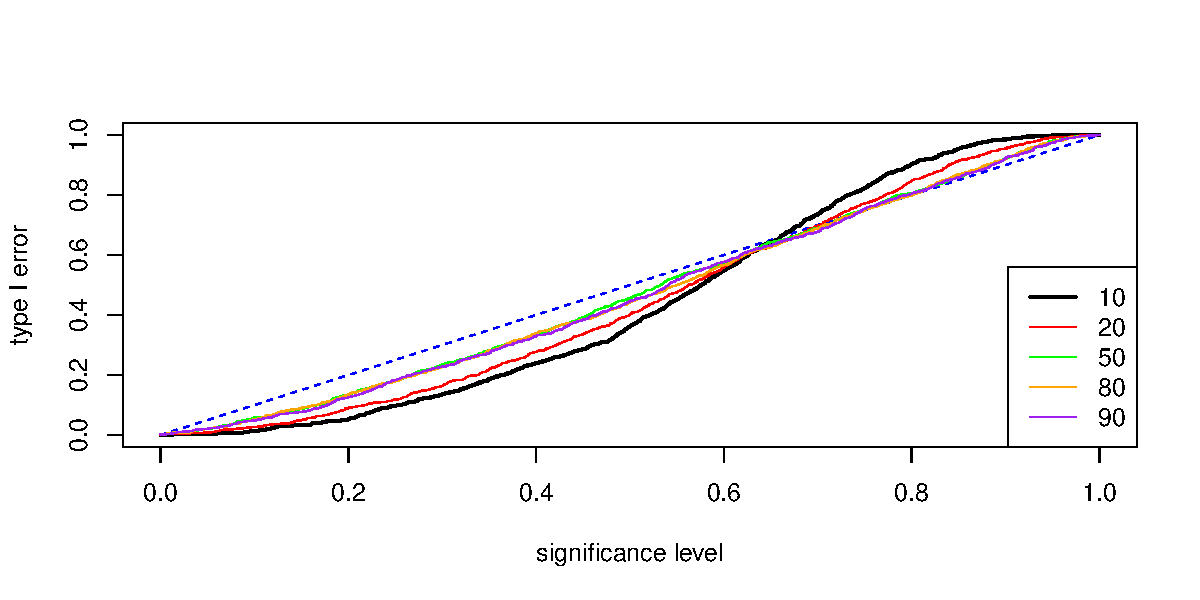
\includegraphics[width=\linewidth]{img/alphaI_cos_est.pdf}
		\caption{Оцененные параметры шума}
	\end{subfigure}
	\caption{Ошибка первого рода для разных длин окна (критерий <<cos>>)}
	\label{fig:alphaI_true_est_cos}
\end{figure}

\subsection{Модификация MC-SSA по части спектра}

Еще одной проблема, возникающая при применении MC-SSA на практике~--- при оценке параметров значениям периодограммы в некоторых частотах нельзя верить. Такая ситуация возникает, например, когда в исходном временном ряде был тренд и, после его выделения, значение периодограммы в низких частотах занижено. Можно убрать не интересующую нас часть спектра, задав диапазоны нерассматриваемых частот $\mathcal{B}=\bigcup\limits_{j}[\omega_{j_1}, \omega_{j_2}]$. Таким образом, в алгоритме~\ref{alg:multiple_mc-ssa} из рассмотрения уйдут все векторы $W_k$, частоты $\omega_k$ которых не попадают в $\mathcal{B}$. Оценка параметров по части спектра возможна, модифицировав правдоподобие Уиттла~\eqref{eq:whittle_loglik}. Пусть $\bm\varphi$ и $\sigma^2$~--- параметры шума $\bm\xi$. Положим $J_{\mathcal{B}^\complement}=\{j \in \{1,\ldots, m\}:~\omega_j=j/N \not\in \mathcal{B}\}$, где $m=\lfloor (N-1)/2 \rfloor$. Тогда правдоподобие Уиттла по части спектра выглядит следующим образом:
\begin{equation}\label{eq:whittle_loglik_par_spectrum}
	\ell_{W_\text{part}}(\bm\varphi, \sigma^2; \mathcal{B})=-\frac{1}{|J_{\mathcal{B}^\complement}|}\sum_{j\in J_{\mathcal{B}^\complement}}\left(\ln f(\omega_j; \bm\varphi, \sigma^2) + \frac{I(\omega_j)}{f(\omega_j; \bm\varphi, \sigma^2)}\right),
\end{equation}
где $f(\omega; \bm\varphi,\sigma^2)$~--- спектральная плотность шума $\bm\xi$, $I(\omega)$~--- периодограмма~\eqref{eq:pgram} исходного временного ряда. В алгоритме~\ref{alg:multiple_mc-ssa_part_spectrum} приведена модификация алгоритма~\ref{alg:multiple_mc-ssa} по части спектра.

\begin{algorithm}[!ht]
	\caption{Multiple MC-SSA по части спектра}\label{alg:multiple_mc-ssa_part_spectrum}
	\Input временной ряд $\tX$, длина окна $L$, набор векторов $W_k\in \R^L$, $\|W_k\|=1$, $k=1,\ldots, H$, модель шума $\bm\xi$, уровень значимости $\alpha$, количество суррогатных реализаций $G$, диапазоны нерассматриваемых частот $\mathcal{B}$.\\
	\Output $H_0$ отвергается/не отвергается, скорректированные интервалы прогнозирования
	\begin{algorithmic}[1]
		\State Если параметры модели $\bm\xi$ неизвестны, оценить их, максимизируя правдоподобие Уиттла по части спектра~\eqref{eq:whittle_loglik_par_spectrum}.
		\State Для $k=1,\ldots,H$ оценить доминирующую частоту $\omega_k$ вектора $W_k$ (например, с помощью ESPRIT~\cite[Раздел 3.1]{SSA_R}).
		\State Применить алгоритм~\ref{alg:multiple_mc-ssa} с векторами $W_k$, $k=1,\ldots, H$ и $\omega_k \not\in \mathcal{B}$.
	\end{algorithmic}
\end{algorithm}

\subsection{Примеры реальных рядов}

Рассмотрим несколько примеров реальных временных рядов с длинной памятью и применим к ним MC-SSA. Оценивать параметры будем теми же методами, что и в разделе~\ref{sect:est_param}.

\subsubsection{Nile Minima}

\begin{figure}[h!]
	\centering
	\subcaptionbox{\label{fig:NileMin_ts}}{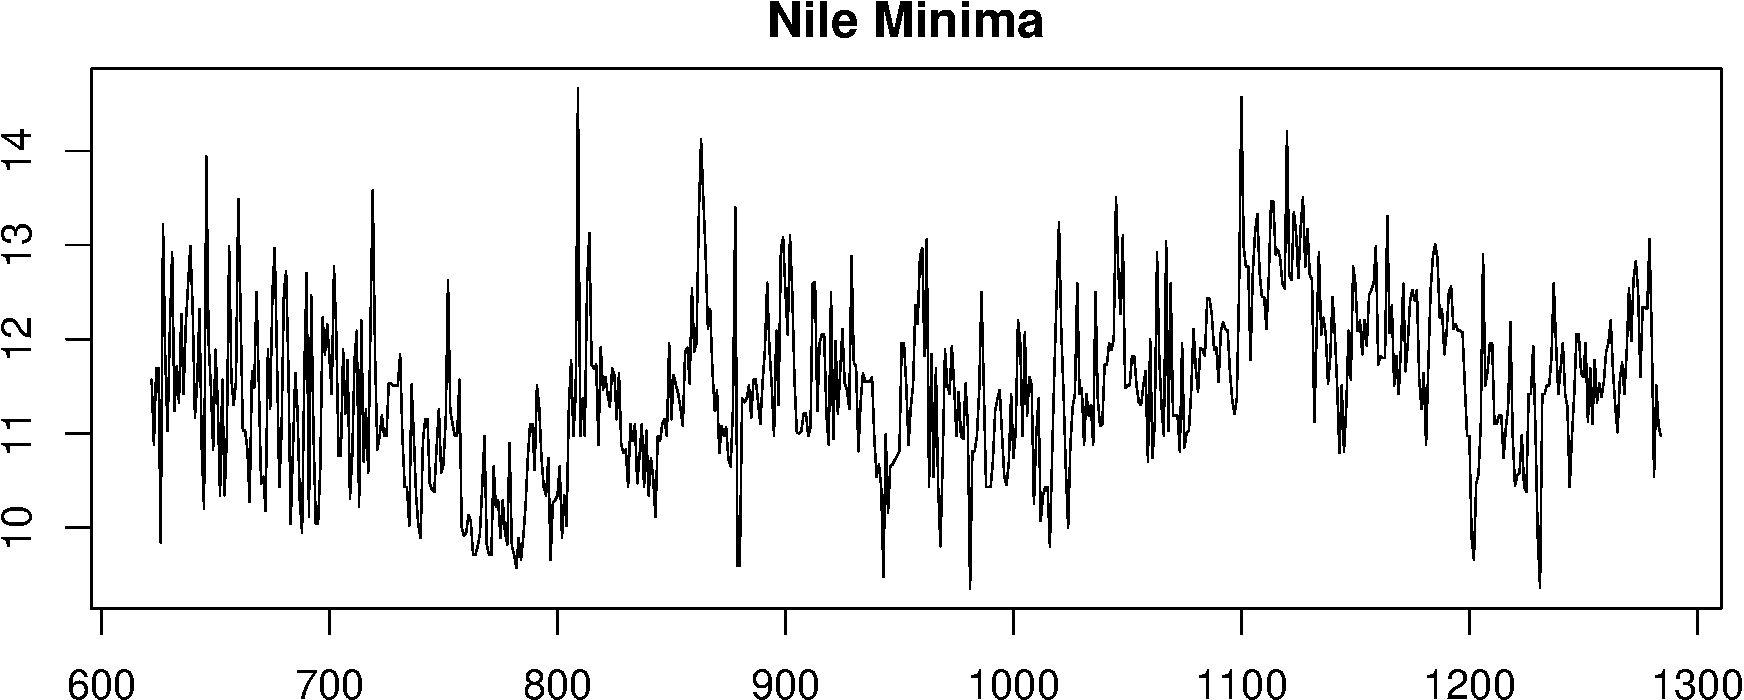
\includegraphics[width=\textwidth]{img/NileMin_ts.pdf}}
	\subcaptionbox{\label{fig:NileMin_acf}}{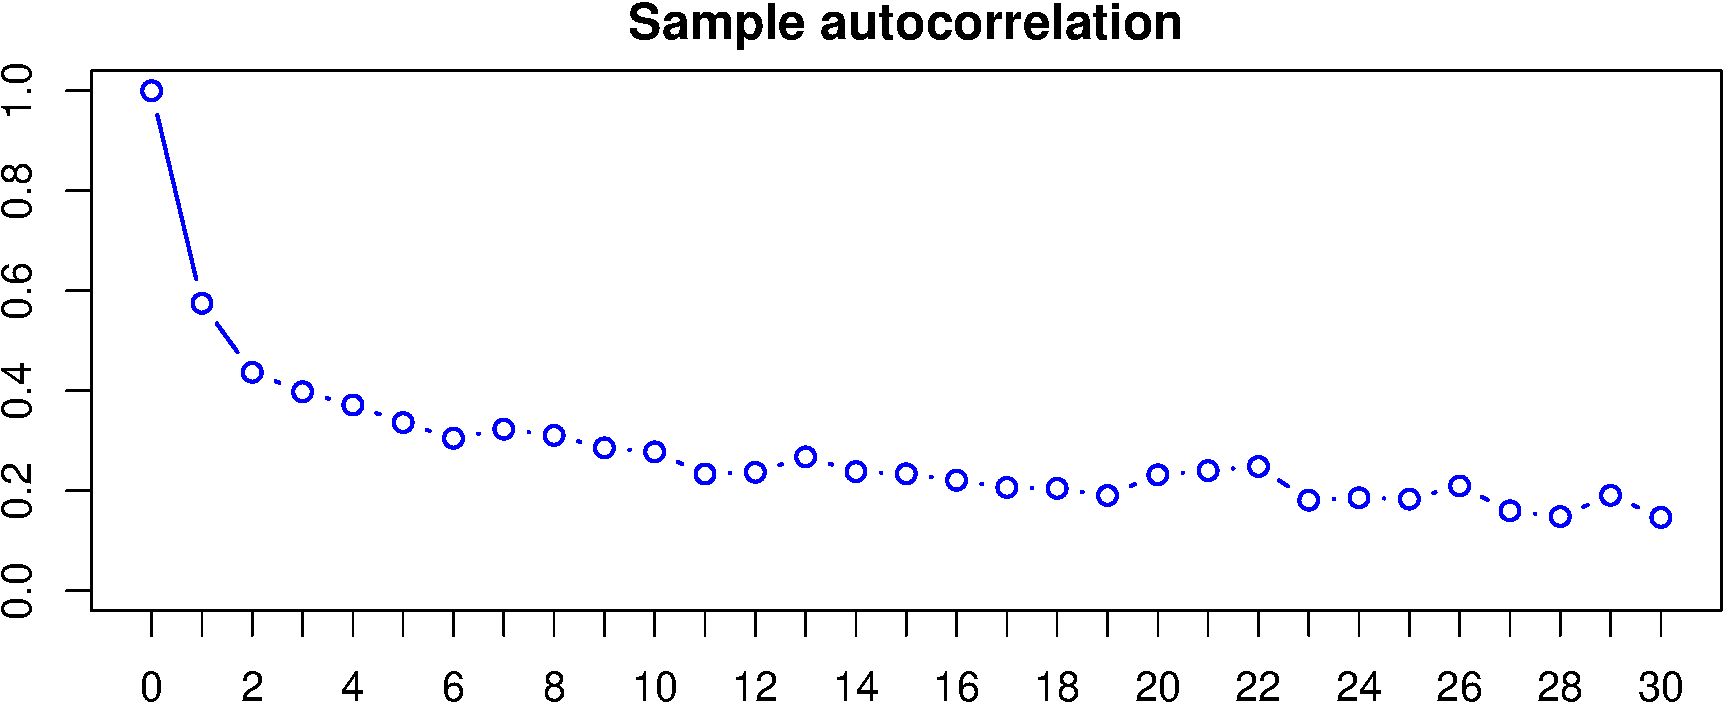
\includegraphics[width=\textwidth]{img/NileMin_acf.pdf}}
	\caption{Ежегодный минимальный уровень воды реки Нил}
\end{figure}

На рис.~\ref{fig:NileMin_ts} изображен ежегодный минимальный уровень воды реки Нил за период с 622 по 1284 год (663 наблюдения), данные были взяты из~\cite{Beran1994}. Нерегулярные циклы или тенденции в этом временном ряду, обусловленные длинной памятью, впервые были обнаружены и обсуждены Хёрстом, британским инженером, который работал гидрологом на реке Нил. Подтверждает присутствие длинной памяти график медленно угасающей автокорреляционной функции на рис.~\ref{fig:NileMin_acf}.

\begin{table}[h]
	\centering
	\caption{Оценка параметров модели $\textrm{ARFIMA}(0, d, 0)$ ряда Nile Minima}
	\label{tab:NileMin_est}
	\begin{tabular}{|c|c|c|}
		\hline
		Метод                  & $\hat{d}$ & $\hat{\sigma}^2$ \\
		\hline
		$\mathrm{MLE}(\bar x)$ & 0.39264   & 0.48939          \\
		H\&R                   & 0.39327   & 0.48934          \\
		Whittle                & 0.40547   & 0.49026          \\
		\hline
	\end{tabular}
\end{table}

\begin{figure}[h]
	\centering
	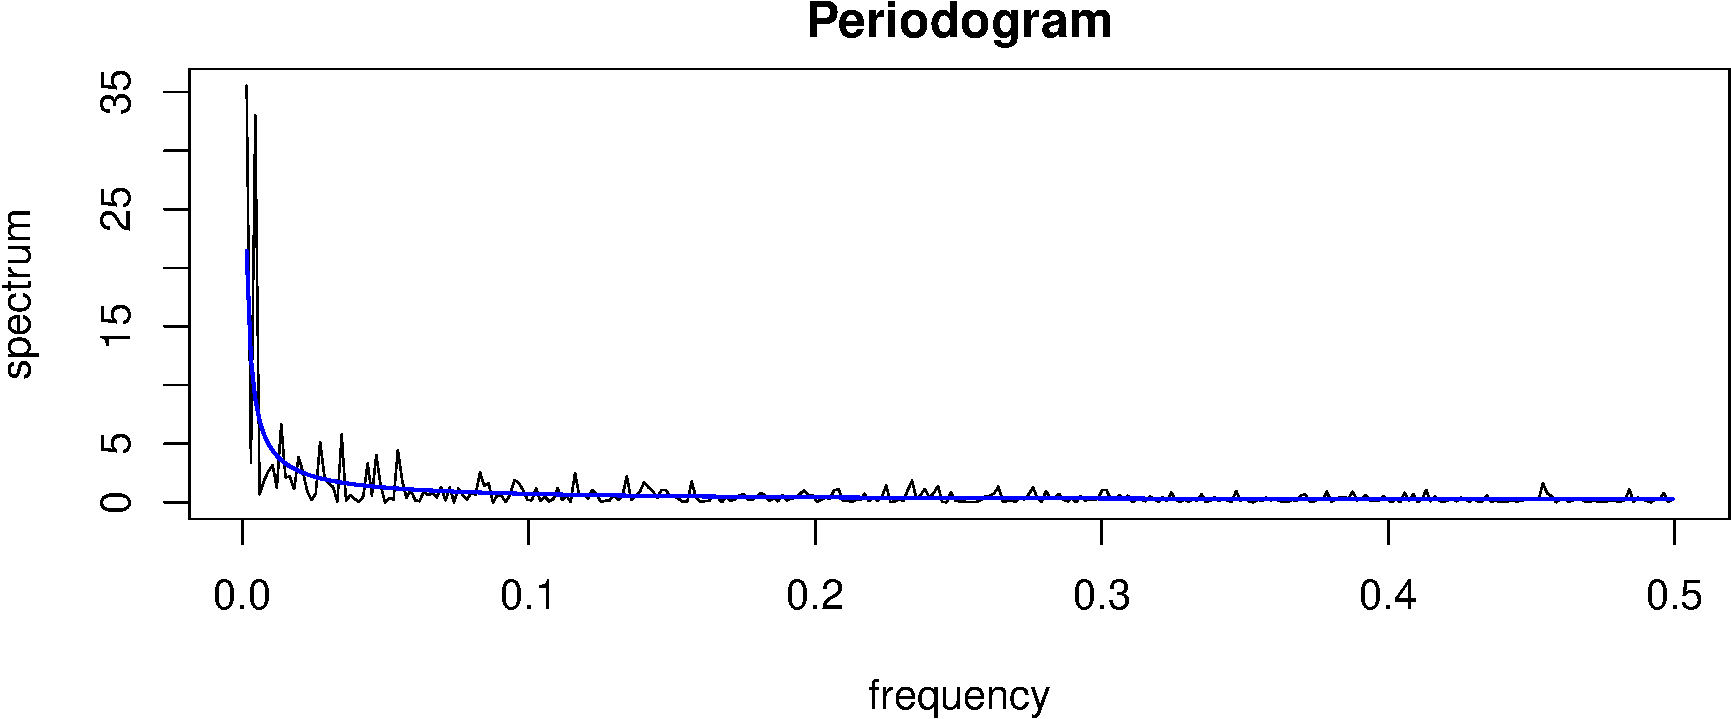
\includegraphics[width=\textwidth]{img/NileMin_per.pdf}
	\caption{Периодограмма ряда Nile Minima}
	\label{fig:NileMin_per}
\end{figure}

Оценим параметры модели $\textrm{ARFIMA}(0, d, 0)$. В таблице~\ref{tab:NileMin_est} представлены оценки параметров $d$ и $\sigma^2$. Поскольку истинное среднее неизвестно и оценка $d$ по Whittle дает наименьшее смещение (см. рис.~\ref{fig:fi_est}), в качестве нулевой гипотезы MC-SSA выберем модель $\textrm{ARFIMA}(0, d, 0)$ с $d=0.40547$ и $\sigma^2=0.48971$, на рис.~\ref{fig:NileMin_per} изображена периодограмма ряда вместе с оцененной спектральной плотностью.

\begin{figure}[h!]
	\centering
	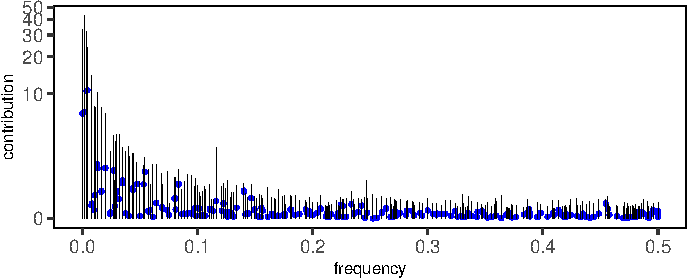
\includegraphics[width=\textwidth]{img/NileMin_mcssa.pdf}
	\caption{Результат работы MC-SSA для ряда Nile Minima}
	\label{fig:NileMin_mcssa}
\end{figure}

Применим MC-SSA с длиной окна $L=330\approx N / 2$. На рис.~\ref{fig:NileMin_mcssa} изображены 95\%-ные доверительные интервалы статистик $\widehat{p}_k$, $k=1,\ldots,L$ (см. алгоритм~\ref{alg:multiple_mc-ssa}). Ни одна из статистик не является значимой, это означает, что нет оснований полагать, что в этом временном ряде присутствует неслучайный сигнал.

\subsubsection{Ireland Wind}

На рис.~\ref{fig:IrelandWind_ts} изображены среднесуточные данные о скорости ветра (в узлах) за период с 1961 по 1978 год ($6574$ дней) на станции Roche's Point в Республике Ирландия~\cite{Haslett1989}.

\begin{figure}[h]
	\centering
	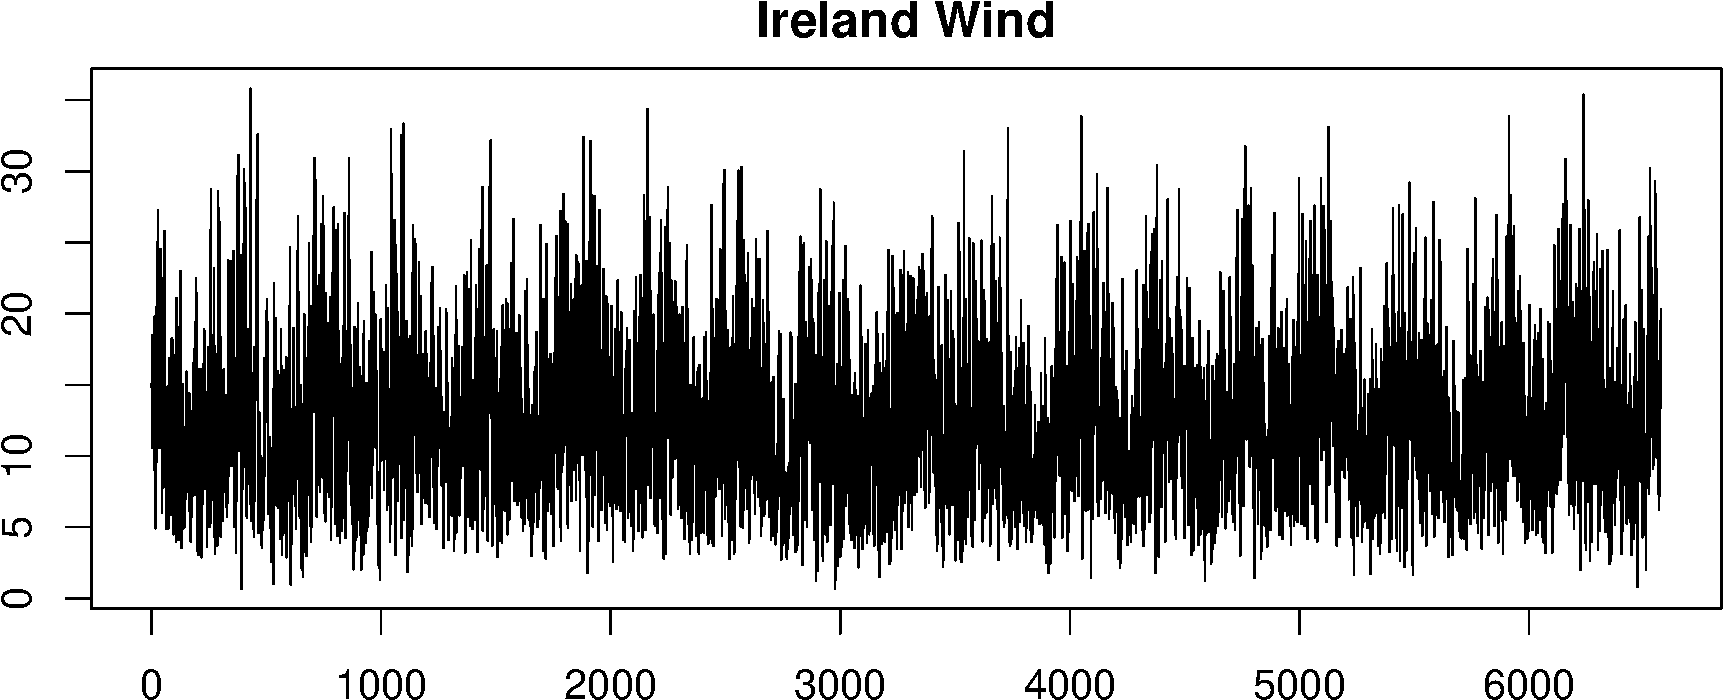
\includegraphics[width=\textwidth]{img/IrelandWind_ts.pdf}
	\caption{Среднесуточные данные о скорости ветра в Республике Ирландия}
	\label{fig:IrelandWind_ts}
\end{figure}

В таблице~\ref{tab:IrelandWind_est} представлены оценки параметров. Полученные оценки примерно одинаковые, но поскольку Whittle дает менее смещенную оценку (см. рис.~\ref{fig:fi_est} и таблицу~\ref{tab:arfi_est_n1000}), будем использовать именно ее.

\begin{table}[h]
	\centering
	\caption{Оценка параметров ряда Ireland Wind}
	\label{tab:IrelandWind_est}
	\begin{tabular}{|c|c|c|c|c|c|}
		\cline{2-6}
		\multicolumn{1}{c|}{}  & \multicolumn{2}{c|}{$\textrm{ARFIMA}(0, d, 0)$} & \multicolumn{3}{c|}{$\textrm{ARFIMA}(1, d, 0)$}                                             \\
		\hline
		Метод                  & $\hat d$                                        & $\hat\sigma^2$                                  & $\hat{d}$ & $\hat\phi$ & $\hat{\sigma}^2$ \\
		\hline
		$\mathrm{MLE}(\bar x)$ & 0.37117                                         & 24.39916                                        & 0.17306   & 0.28403    & 23.7581          \\
		H\&R                   & 0.36891                                         & 24.38116                                        & 0.17245   & 0.28309    & 23.73458         \\
		Whittle                & 0.37287                                         & 24.40285                                        & 0.17598   & 0.28105    & 23.75983         \\
		\hline
	\end{tabular}
\end{table}

\begin{figure}[h]
	\centering
	\subcaptionbox{$\textrm{ARFIMA}(0, d, 0)$\label{fig:IrelandWind_mcssa_fi}}{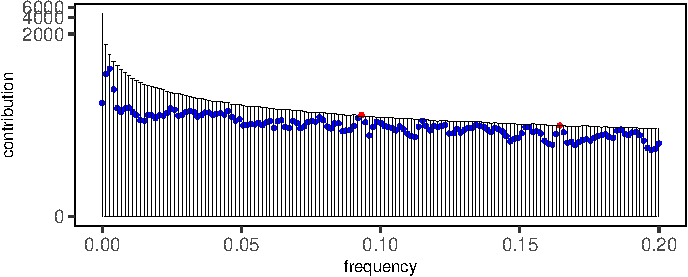
\includegraphics[width=\textwidth]{img/IrelandWind_mcssa_fi.pdf}}
	\subcaptionbox{$\textrm{ARFIMA}(1, d, 0)$\label{fig:IrelandWind_mcssa_arfi}}{
\includegraphics[width=\textwidth]{img/IrelandWind_mcssa_arfi.pdf}}
	\caption{Результат работы MC-SSA для ряда Ireland Wind}
	\label{fig:IrelandWind_mcssa}
\end{figure}

Поскольку ряд достаточно длинный, чтобы не делать поправку, рассмотрим в качестве векторов для проекции косинусы с равноотстоящими частотами, определенные в формуле~\eqref{eq:cos_proj_vectors}. Также выберем длину окна не слишком большой, чтобы метод MC-SSA считался за адекватное время, скажем, $L=365$. На рис.~\ref{fig:IrelandWind_mcssa} представлен результат работы MC-SSA для обоих моделей, уровень значимости, как и в прошлом примере, равен $\alpha = 0.05$. Для модели $\textrm{ARFIMA}(0, d, 0)$ значимых векторов два, их периоды равны $365 / 34\approx10.74$ и $365 / 60\approx6.08$ дней соответственно, что сложно как-то интерпретировать. Однако стоит заметить, что вклады значимых векторов не слишком превосходят верхние границы соответствующих предсказательных интервалов, поэтому, скорее всего, векторы значимы случайно (количество случайно значимых векторов в среднем равно $\alpha \cdot L=18.25$). В случае модели $\textrm{ARFIMA}(1, d, 0)$ значим всего один вектор с периодом $365$ дней, что интерпретируется как наличие во временном ряде годовой периодичности.


\chapter{Методы автоматической идентификации компонент}\label{chpt:auto_ssa}

Важной проблемой метода SSA является автоматическая идентификация компонент на этапе группировке. На данный момент, существуют методы автоматической идентификации, основанные на частотных характеристиках компонент, описанные в работах~\cites[Section 2.7]{SSA_R}{Vautard1992}{AlexandrovGolyandina2004}. В частности, методы основаны на доле значений периодограммы компоненты разложения в выбранном диапазоне частот. Тренд определяется как низкочастотная составляющая ряда, на чем основан частотный метод автоматической идентификации~\cites[Section 2.7]{SSA_R}{AlexandrovGolyandina2004}. Что касается периодических компонент, то в частотном подходе нужно знать периоды, что часто нереализуемо, а также мешает возможная амплитудная модуляция входящих в периодику гармоник, что приводит к растеканию по частотам в периодограмме.

Для решения проблемы неизвестных частот периодик используется свойство SSA разложения, состоящее в том, что экспоненциально-модулированной гармоники кроме случая частоты 0.5 соответствуют две компоненты с той же модуляцией и той же частотой. На этом основан периодограммный метод~\cite{Vautard1992}, который использует это свойство. Однако метод не решает проблемы растекания частот при амплитудной модуляции. Для решения этой проблемы в работах~\cite{Zhornikova2018,GolyandinaZhornikova2023} был предложен метод регулярности углов.

Таким образом, в качестве основных методов мы будет использовать частотный метод для идентификации трендовых и периодических компонент и метод регулярности углов для выделения гармоник. Эти методы описаны в разделе~\ref{sect:grouping_auto} и~\ref{sect:angle_reg}.

При применении методов идентификации компонент существуют две проблемы. Первая~--- это выбор числа первых компонент для идентификации, чтобы идентифицировать только компоненты сигнала или минимально затрагивать шумовые компоненты. Для решения этой проблемы существуют два пути: использование информационных критериев для определения ранга сигнала~\cite{GolyandinaZvonarev2024} и использование такого числа первых компонент, что проверка остатка на отсутствие шума не отвергается некоторым критерием. Для обоих вариантов требуется задавать модель шума и, к сожалению, это не преодолеть.

Для проверки остатка на отсутствие сигнала мы будем рассматривать критерий Monte Carlo SSA~\cite{Allen1996}, описанный в разделе~\ref{sect:mcssa} и обладающий высокой мощностью~\cite{Poteshkin2024}. К его недостаткам можно отнести высокую трудоемкости. В качестве модели шума может быть выбран красный или белый шум, а также процесс с длинной памятью, определенный в разделе~\ref{sect:longmemory}. В любом случае, точно определить число сигнальных компонент сложно ввиду приближенного соответствия реальных временных рядов модели. В этом случае рекомендуется завышать число сигнальных компонент и поэтому методы должны быть устойчивы к включению в число рассматриваемых компонент шумовых компонент.

Вторая общая проблема SSA~--- это смешивание компонент между собой, что мешает идентификации, как визуальной, так и автоматической. Существуют разные модификации метода SSA, которые позволяют делать преобразование сигнальных компонент разложения~\cite{GolyandinaShlemov15, Shlemov2017, autoSSA}, такие как IOSSA, FOSSA и EOSSA. После переразложения сигнальных компонент сигнальные компоненты разложения становятся хорошо разделимыми и пригодными для идентификации. Хорошо работающий метод автоматической идентификации трендовых компонент~\cite{autoSSA} состоит из задания сингулярных компонент с превышением ранга, затем улучшения разделимости методом EOSSA и частотной идентификации трендовых компонент. Так как частотный диапазон тренда довольно узкий и известный, то при завышении числа сигнальных компонент метод работает довольно хорошо~\cite{autoSSA}. Проблема возникает при применении той же идеи к выделению гармоник, так как даже шумовые компоненты начинают разделяться и идентифицироваться как гармонические.

В работе~\cite{Dudnik2025} предлагается алгоритм выделения гармонических компонент, который  решает эту проблему с помощью критерия проверки остатка на отсутствие сигнала. В результате был построен алгоритм, названный SSA-Aid, который может идентифицировать компоненты сигнала и периодик. Алгоритм приведен в разделе~\ref{sect:ssa_aid}

В данной главе под MC-SSA будем подразумевать алгоритм~\ref{alg:multiple_mc-ssa_part_spectrum} с косинусами~\eqref{eq:cos_proj_vectors} в качестве векторов для проекции.

\section{Автоматическая группировка в SSA}\label{sect:grouping_auto}

Для периодограммы~\eqref{eq:pgram} вещественного временного ряда справедливо:
\[
	I(\omega)=I(1-\omega), \quad \forall \omega,
\]
то есть периодограмма вещественного ряда симметрична относительно частоты $0.5$. Введем понятие односторонней периодограммы $\Pi$:
\begin{equation}\label{eq:pgram_corrected}
	\Pi(k / N)=
	\begin{cases}
		I(k / N) + I(1 - k / N), & \text{для } 0<k<N/2, \\
		I(k / N),                & \text{иначе}.
	\end{cases}
\end{equation}
Односторонняя периодограмма обладает следующим свойством:
\[
	\|\tX\|^2=\sum_{n=1}^N x_n^2=\sum_{k=0}^{\lfloor N/2\rfloor} \Pi(k / N).
\]
Таким образом, односторонняя периодограмма сохраняет полную энергию, учитывая симметричность обычной (двусторонней) периодограммы для вещественных рядов.

Для ряда $\tX$ длины $N$ и $0\leqslant\omega_1\leqslant\omega_2\leqslant0.5$ определим меру, следуя~\cite{AlexandrovGolyandina2004}:
\begin{equation}\label{eq:freq_measure}
	T(\tX;\omega_1,\omega_2)=\frac{1}{\|\mathsf{X}\|^2}\sum_{k:\omega_1\leqslant k/N\leqslant \omega_2}\Pi(k/N).
\end{equation}
Поскольку $\|\tX\|^2=\sum_{k=0}^{\lfloor N/2\rfloor} \Pi(k / N)$, величину $T(\tX,\omega_1,\omega_2)$ можно рассматривать как долю вклада частот, содержащегося в интервале $[\omega_1,\omega_2]$.

\subsection{Автоматическая идентификация тренда}

Поскольку тренду соответствуют низкие частоты, можно относить к тренду те компоненты разложения, у которых вклад низких частот больше некоторого порога. Приведем алгоритм автоматической идентификации тренда, описанный в~\cite{AlexandrovGolyandina2004}.

\begin{algorithm}[H]
	\caption{TAI$(\omega_0, T_\text{low})$~\cite{AlexandrovGolyandina2004}}\label{alg:auto_trend}
	\Input элементарные восстановленные компоненты $\tX^{(j)}$, $j\in J$, порог низких частот $\omega_0$, порог вклада низких частот $T_\text{low}\in[0, 1]$.\\
	\Output индексы компонент, относящихся к тренду, оценка тренда $\hat\tT$.
	\begin{algorithmic}[1]
		\State Вычислить $T_j=T(\tX^{(j)};0,\omega_0)$ для каждого $j\in J$.
		\State Определить компоненты $J_\text{Trend}=\{j\in J:~T_j > T_\text{low}\}$, относящиеся к тренду, вычислить оценку тренда $\hat \tT=\sum\limits_{j\in J_\text{Trend}} \tX^{(j)}$.
	\end{algorithmic}
\end{algorithm}

\subsection{Автоматическая идентификация периодики}

По аналогии с алгоритмом~\ref{alg:auto_trend} можно выделять и периодики. Приведем в алгоритме~\ref{alg:auto_periodic} алгоритм идентификации периодики по заданной частоте.

\begin{algorithm}[!ht]
	\caption{Алгоритм идентификации периодики по заданной частоте}\label{alg:auto_periodic}
	\Input Ряды $\tX^{(j)}$, $j\in J$, частота $\omega\in(0, 0.5]$, радиус $\delta \geqslant 0$, порог $T_0\in[0, 1]$, количество компонент $d$. \\
	\Output Индексы рядов, относящихся к периодике с частотой $\omega$, оценка $\hat\tP$.
	\begin{algorithmic}[1]
		\State Вычислить $T_j=T(\tX^{(j)};\omega - \delta,\omega + \delta)$ для каждого $j\in J$.
		\State Из множества $J_\text{signif}=\{j\in J:~T_j > T_0\}$ выбрать $\min(d, |J_\text{signif}|)$ элементов, соответствующих рядам с наибольшим $\mathsf{MSS}\left(\tX^{(j)}\right)=\frac{1}{N}\sum^{N}_{i=1}\left(x^{(j)}_i\right)^2$. Обозначим множество этих индексов за $J_\text{Periodic}$.
		\State Вычислить оценку периодики $\hat \tP=\sum\limits_{j\in J_\text{Periodic}} \tX^{(j)}$.
	\end{algorithmic}
\end{algorithm}

\begin{remark}
	В алгоритме~\ref{alg:auto_periodic} ряды $\tX^{(j)}$ не обязательно являются элементарно восстановленными компонентами. Это могут быть уже сгруппированные (например, с помощью метода регулярности углов~\cite{GolyandinaZhornikova2023}) ряды: в таком случае $d=1$. Если $\tX^{(j)}$~--- элементарные восстановленные компоненты, то, учитывая, что экспоненциально-моделированная гармоника~\eqref{eq:em_harmonic} описывается одной или двумя элементарными восстановленными компонентами, в качестве параметра $d$ логично взять
	\begin{equation}\label{eq:d_cos}
		d_{\cos}(\omega)=
		\begin{cases}
			2, & \text{для } \omega\in(0, 0.5), \\
			1, & \text{иначе}.
		\end{cases}
	\end{equation}
\end{remark}

\begin{remark}
	Недостаток алгоритма~\ref{alg:auto_periodic} заключается в необходимости знать частоты, соответствующие сигналу, что часто нереализуемо. Также заметим, что амплитудная модуляция сигнала приводит к растеканию вклада по частотам периодограммы, что влечет за собой проблему выбора радиуса $\delta$. Однако первый недостаток не является проблемой, поскольку MC-SSA позволяет определять значимые частоты. Этот факт используют методы autoMCSSA и SSA-AidMC, описанные в разделе~\ref{sect:autoMCSSA} и~\ref{sect:ssa_aid_mc} соответственно.
\end{remark}

\section{Метод идентификации колебательной составляющей по регулярности углов}\label{sect:angle_reg}

Идея данного метода идентификации колебательной составляющей была предложена в работе~\cite{Zhornikova2018} и подробно описана в статье~\cite{GolyandinaZhornikova2023}, в работе~\cite{Dudnik2025} была предложена модификация метода. Метод основывается на свойствах следующих специальных мер:

\begin{enumerate}
	\item Для векторов $P = (p_1,\ldots,p_L)^{\mathrm{T}}$, $Q=(q_1,\ldots,q_L)^{\mathrm{T}}\in\R^L$ определим меру $\tau$:
	      \begin{equation}\label{eq:tau_measure}
		      \tau(P, Q) = \hat{\mathsf{D}}(\Theta) =\frac{1}{L-1}\sum_{k=1}^{L-1}{\left(\theta_k  - \bar{\theta}\right)^2},
	      \end{equation}
	      где $\Theta=(\theta_1,\ldots,\theta_L)^{\mathrm{T}}$,
	      $\bar{\theta} = \sum_{k=1}^{L-1}{\theta_k}/(L-1)$, $\theta_k$ --- угол между
	      $\left(p_k, q_{k}\right)^{\mathrm{T}}$ и $\left(p_{k+1}, q_{k+1}\right)^{\mathrm{T}}$, т.е.
	      \begin{gather*}
		      \theta_k = \arccos{\left(\frac{p_{k} p_{k+1} + q_{k} q_{k+1}}{\sqrt{p_{k}^2+q_{k}^2}\sqrt{p_{k+1}^2+q_{k+1}^2}}\right)}.
	      \end{gather*}
	\item Для вектора $U = (u_1,\ldots,u_L)^\rmT\in\R^L$ определим меру $\gamma$:
	      \begin{equation}\label{eq:gamma_measure}
		      \gamma(U) = \frac{1}{L - 1}\sum_{i = 1}^{L - 1}(\mathsf{sign}(u_i) + \mathsf{sign}(u_{i + 1})).
	      \end{equation}
\end{enumerate}

Мера $\tau$ показывает насколько различаются углы между последовательными точками $(p_k, q_k)^\rmT$ двумерной диаграммы векторов $P$ и $Q$ и равное нулю значение меры говорит о принадлежности векторов к одной гармонике. Равное нулю значение меры $\gamma$, в свою очередь, говорит о том, что последовательные точки разные по знаку, что свойственно гармонике с периодом $2$ (частоте $0.5$).

Поскольку в ряде обычно, помимо сигнальных компонент, присутствует шум, необходимо ввести для этих мер пороги. Приведем в алгоритме~\ref{alg:angle_reg} модификацию алгоритма идентификации колебательной составляющей по регулярности углов.

\begin{algorithm}
	\caption{Модифицированный метод регулярности углов~\cite{Dudnik2025}}\label{alg:angle_reg}
	\Input линейно независимые векторы $\{U_j\}_{j=1}^r$, порог $t_0\geqslant0$, порог $p_0\geqslant0$.
	\Output множество индексов $J_\text{Periodics}$, относящихся к колебательной составляющей.
	\begin{algorithmic}[1]
		\State Составить множество индексов, соответствующее периодикам с частотой $\omega=0.5$:
		\[
			J_1=\{i\in J: \gamma(U_i)<p_0\}.
		\]
		\State Перенумеровать оставшиеся векторы $\{U\}_{j\in \{1,\ldots, r\}\setminus J_1}$: $\{U^\prime\}_{j=1}^{r_2}$, где $r_2=r-|J_1|$.
		\State Вычислить значение $\tilde\tau_j=\tilde \tau(U^\prime_j, U^\prime_{j+1})$, $j=1,\ldots,r_2-1$:
		\[
			\tilde \tau(P, Q)=\frac{\tau(P, Q)}{\min(1,\overline\theta^2)},
		\]
		где мера $\tau(P, Q)$ определена в формуле~\eqref{eq:tau_measure}.
		\State $J_2\coloneq \varnothing$. Для $i=1,\ldots,r_2-1$:
		\begin{algsubstates}
			\State Если $\tilde\tau_i < t_0$ и оба индекса $j$, $j+1$ не были отобраны ранее, $J_2 \coloneq J_2 \cup \{(j, j+1)\}$.
		\end{algsubstates}
		\State Множество $J_{Periodics} \coloneq J_1\cup J_2$ состоит из кортежей размера $1$ (случай частоты $\omega = 0.5$) и кортежей размера $2$ (случай частоты $\omega \neq 0.5$).
	\end{algorithmic}
\end{algorithm}

% \section{Метод автоматической идентификации тренда и периодик}

% Для борьбы с неразделимостью компонент предложили использовать вложенное (nestled) разложение матрицы $\bfX$, семейство этих методов~--- Oblique SSA~\cite{SSA_R}. Самым новым и удобным на практике является метод EOSSA (ESPRIT-based Oblique SSA)~\cite{Shlemov2017}.

% Приведем алгоритм~\ref{alg:auto_periodic_trend}, который сначала применяет переразложение сигнальных компонент для улучшения разделимости, а затем разбивает множество индексов компонент на два непересекающихся подмножества: на трендовые и на периодические. Этот алгоритм будет использоваться в дальнейшем при описании других, более сложных, методов автоматической идентификации.

% На его основе уже был предложен метод автоматической идентификации компонент: SSA-Aid~\cite{Dudnik2025}. Приведем описание метода в алгоритмах~\ref{alg:auto_periodic_trend},~\ref{alg:auto_periodic_trend_mc} и~\ref{alg:auto_ssa}, на которые будем ссылаться далее.

% \begin{algorithm}[!ht]
% 	\caption{Алгоритм автоматической идентификации трендовых и периодических компонент~\cite{Dudnik2025}}\label{alg:auto_periodic_trend}
% 	\Input временной ряд $\tX$, длина окна $L_\text{SSA}$, оценка ранга сигнала $r$, порог $t_0$, порог $p_0$, порог низких частот $\omega_0$, порог вклада низких частот $T_{\text{low}}$.\\
% 	\Output Множества индексов, соответствующие тренду и периодикам.
% 	\begin{algorithmic}[1]
% 		\State Применить к исходному ряду алгоритм autoEOSSA($r, \omega_0, T_{\text{low}}$)~\cite{autoSSA}. Результат: множество индексов $J_\text{Trend}$, которое соответствует тренду.
% 		\State Применить к компонентам с индексами из множества $J\setminus J_\text{Trend}$ модифицированный метод регулярности углов (алгоритм~\ref{alg:angle_reg}). Результат: множество индексов $J_\text{Periodics}$, которое соответствует периодикам.
% 	\end{algorithmic}
% \end{algorithm}

\section{Метод SSA-Aid}\label{sect:ssa_aid}

Главная проблема алгоритмов~\ref{alg:auto_trend},~\ref{alg:auto_periodic} и~\ref{alg:angle_reg} заключается в возможном смешивании спектров сигнальных компонент, в таком случае приведенные подходы перестают корректно работать. Для решения этой проблемы используют методы переразложения для улучшения разделимости, в частности, алгоритм EOSSA~\cite{Shlemov2017}.

В работе~\cite{autoSSA} показано, что оценка тренда устойчива к завышению ранга сигнала $r$. Однако это неверно для оценки периодик: при применении EOSSA компоненты, соответствующие шуму, становятся похожими на периодики. В работе~\cite{Dudnik2025} был предложен метод SSA-Aid, который использует статистический критерий для проверки гипотезы об отсутствии сигнала для отбора сигнальных периодик. Приведем описание метода в алгоритмах~\ref{alg:auto_periodics},~\ref{alg:auto_periodic_trend} и~\ref{alg:auto_ssa}. На рис.~\ref{fig:ssa_aid_flowchart} представлена блок-схема одной итерации SSA-Aid (алгоритма~\ref{alg:auto_periodic_trend}). Как уже можно было заметить, метод SSA-Aid итеративно вычисляет оценку ранга сигнала, поэтому метод устойчив к завышению ранга сигнала $r$. Также заметим, что в оригинальной работе~\cite{Dudnik2025} используется произвольный статистический критерий проверки гипотезы об отсутствии сигнала, однако для простоты описания алгоритмов положим в качестве критерия метод MC-SSA, который превосходит по мощности другие критерии проверки гипотезы об отсутствии сигнала~\cite{Poteshkin2024} и с помощью которого можно определенить значимые частоты. Эту особенность критерия будем использовать в последующих разделах.

\begin{algorithm}[!htbp]
	\caption{Алгоритм отбора гармоник, испольщующий критерий для проверки гипотезы о наличии сигнала в шуме~\cite{Dudnik2025}}\label{alg:auto_periodics}
	\Input Ряд без тренда $\tX^\prime$, элементарные восстановленные компоненты $\tX^{(j)}$, $j\in J$, длина окна $L_\text{MC-SSA}$, модель шума $\bm\xi$, уровень значимости $\alpha$, порог низких частот $\omega_0$.
	\Output Оценка периодик $\hat \tP$, оценка ранга периодик $\hat r_\text{Periodics}$.
	\begin{algorithmic}[1]
		\State Инициализировать оценку периодик $\hat{\tP}$ нулевым рядом, оценку ранга периодической компоненты $\hat{r}_\text{Periodics} \coloneq 0$ и диапазоны нерассматриваемых частот $\mathcal{B} \coloneq [0, \omega_0]$.
		\State Применить алгоритм~\ref{alg:multiple_mc-ssa_part_spectrum} к ряду $\tX^\prime$ с длиной окна $L_\text{MC-SSA}$. Если нулевая гипотеза не отвергается при уровне значимости $\alpha$, завершить работу алгоритма.
		\State Применить к компонентам с индексами из множества $J$ модифицированный метод регулярности углов (алгоритм~\ref{alg:angle_reg}). Результат: множество индексов $J_\text{Periodics}$, которое соответствует периодикам.
		\State Восстановить компоненты, используя множество $J_{\text{Periodics}}$ и ранжируем по величине $\mathsf{MSS}\left(\tX^{(j)}\right)=\frac{1}{N}\sum^{N}_{i=1}\left(x^{(j)}_i\right)^2$ по убыванию. Пусть восстановлено $n_{\mathsf{id}} = |J_{\text{Periodics}}|$ компонент и $\left\{\tX^{(j)}\right\}_{j=1}^{n_{\mathsf{id}}}$~--- полученный набор. Этому набору соответствует множество рангов  $\left\{r_p^{(j)}\right\}_{j=1}^{n_{\mathsf{id}}}$.
		\State Для $j = 1, \ldots, n_{\mathsf{id}}$:
		\begin{algsubstates}
			\State $\hat{\tP} \coloneq \hat{\tP} + \tX^{(j)}$. $\hat{r}_\text{Periodics} \coloneq \hat{r}_\text{Periodics}+r_p^{(j)}$, $\hat{\tN} \coloneq \tX^\prime - \hat{\tP}$.
			\State Применить к остатку $\hat{\tN}$ алгоритм~\ref{alg:multiple_mc-ssa_part_spectrum}. Если гипотеза не отвергается при уровне значимости $\alpha$, завершить работу алгоритма.
		\end{algsubstates}
	\end{algorithmic}
	
\end{algorithm}

\begin{algorithm}[!htbp]
	\caption{Алгоритм автоматической идентификации компонент, использующий критерий для проверкой гипотезы о наличии сигнала в шуме~\cite{Dudnik2025}}\label{alg:auto_periodic_trend}
	\Input временной ряд $\tX$, длина окна $L_\text{SSA}$, длина окна $L_\text{MC-SSA}$, модель шума $\bm\xi$, оценка ранга сигнала $r$, порог $t_0$, порог $p_0$, уровень значимости $\alpha$, порог низких частот $\omega_0$, порог вклада низких частот $T_{\text{low}}$.\\
	\Output разложение оценки сигнала в сумму тренда и периодик $\hat{\tS}=\hat{\tT} + \hat{\tP}$, уточненная оценка ранга сигнала $\hat{r}=\hat{r}_\text{Trend} + \hat{r}_\text{Periodics}$.
	\begin{algorithmic}[1]
		\State Применить к исходному ряду алгоритм autoEOSSA($r, \omega_0, T_{\text{low}}$)~\cite{autoSSA}. Результат: множество индексов $J_\text{Trend}$, которое соответствует тренду, оценка тренда $\hat\tT$, оценка ранга тренда $\hat{r}_\text{Trend}=|J_\text{Trend}|$.
		\State Применить алгоритм~\ref{alg:auto_periodics} с $\tX^\prime = \tX - \hat\tT$ и $J=\{1,\ldots,r\} \setminus  J_\text{Trend}$. Результат: оценка периодики $\hat\tP$, оценка ранга периодик $\hat{r}_\text{Periodics}$.
	\end{algorithmic}
\end{algorithm}

\begin{algorithm}[!htbp]
	\caption{Алгоритм SSA-Aid с обновляемой оценкой ранга сигнала~\cite{Dudnik2025}}\label{alg:auto_ssa}
	\Input временной ряд $\tX$, алгоритм автоматической идентификации компонент $\mathcal{A}$, параметры алгоритма $\mathcal{A}$.\\
	\Output разложение оценки сигнала в сумму тренда и периодик $\hat{\tS}=\hat{\tT} + \hat{\tP}$, уточненная оценка ранга сигнала $\hat{r}$.
	\begin{algorithmic}[1]
		\State Инициализируем оценку ранга сигнала $\hat{r}_\text{input}^{(0)} \coloneq r, i \coloneq 0$.
		\State \label{stage2_auto_ssa}Применить к ряду $\tX$ алгоритм $\mathcal{A}$ с оценкой ранга сигнала $r=\hat{r}_\text{input}^{(i)}$. Результат: разложение оценки сигнала в сумму тренда и периодик $\hat{\tS}^{(i)}=\hat{\tT}^{(i)}+\hat{\tP}^{(i)}$ и оценку ранга $\hat{r}_\text{output}^{(i)}$.
		\State  Если $\hat{r}_\text{input}^{(i)}=\hat{r}_\text{output}^{(i)}$, завершить работу алгоритма с $\hat\tS=\hat{\tS}^{(i)}$ и $\hat{r}=\hat{r}_{output}^{(i)}$.
		\State $\hat{r}_\text{input}^{(i+1)} \coloneq \hat{r}_\text{output}^{(i)}, i \coloneq  i + 1$, перейти к шагу~\ref{stage2_auto_ssa}.
	\end{algorithmic}
\end{algorithm}

\begin{figure}[htbp]
	\centering
	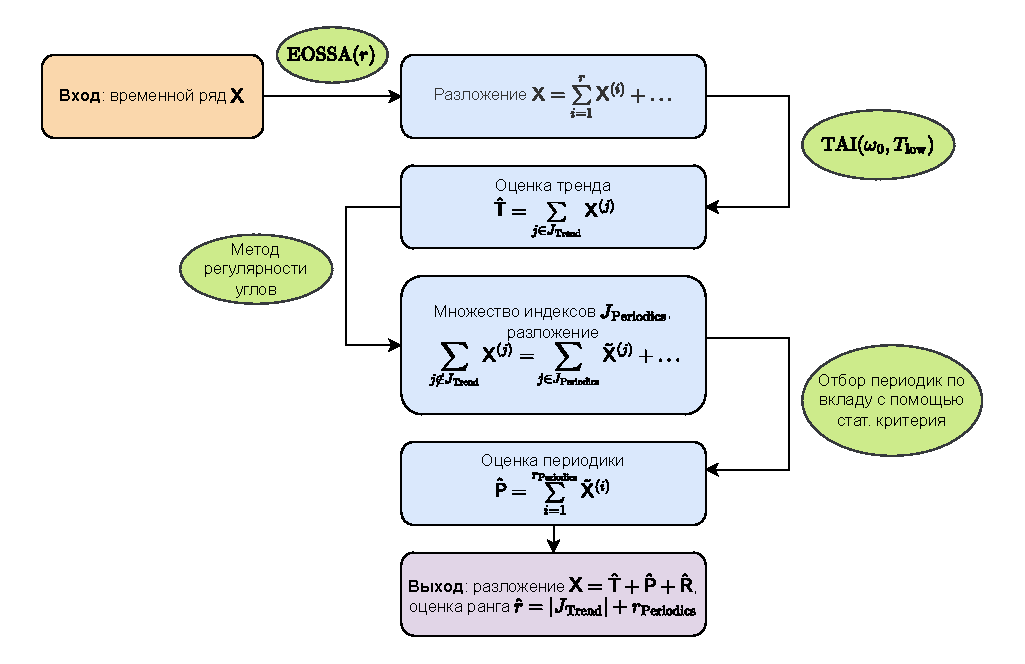
\includegraphics[width=\textwidth]{img/ssa_aid_flowchart.pdf}
	\caption{Блок-схема одной итерации SSA-Aid}
	\label{fig:ssa_aid_flowchart}
\end{figure}

\chapter{Методы автоматической идентификации компонент, использующие критерий MC-SSA для оценки частоты сигнала}

Проблема автоматической идентификации компонент на этапе группировки кажется решенной, однако есть случай, который не охватывается алгоритмами, описанными в главе~\ref{chpt:auto_ssa}: когда сигнальные компоненты идут не подряд. То есть сначала идут сигнальные компоненты, включая трендовые, потом какое-то количество шумовых, а потом снова сигнальные.

Целью данной работы является расширение алгоритма SSA-Aid~\cite{Dudnik2025}, который будет учитывать и этот случай. Этот алгоритм назовем SSA-AidMC, так как он существенно использует метод Monte Carlo SSA~\cite{Allen1996}. Заметим, что алгоритм SSA-Aid также использует метод MC-SSA, однако в SSA-Aid метод MC-SSA используется только как хороший критерий проверки гипотезы об отсутствии сигнала в остатке, а в методе SSA-AidMC он используется для определения частот, которые соответствуют сигналу.

Описание алгоритма SSA-AidMC и его идеи содержится в разделе~\ref{sect:ssa_aid_mc}. Перед этим в разделе~\ref{sect:autoMCSSA} описан алгоритм autoMCSSA выделения компонент сигнала, не обязательно первых, который составляет основу идеи расширения метода SSA-Aid до SSA-AidMC.

В данной главе, как и в предыдущей, под MC-SSA будем подразумевать алгоритм~\ref{alg:multiple_mc-ssa_part_spectrum} с косинусами~\eqref{eq:cos_proj_vectors} в качестве векторов для проекции.

\section{Метод autoMCSSA}\label{sect:autoMCSSA}

% После проверки гипотезы $H_0:\tS=0$ возникает проблема выделения сигнала, если $H_0$ отвергается. Поскольку с помощью критерия MC-SSA можно определить значимые частоты, воспользуемся этим.

\subsection{Мощность MC-SSA в случае сложного сигнала}\label{sect:composite_signal_power}

Давайте рассмотрим следующий сигнал $\tS=(s_1,\ldots, s_N)$:

\begin{example}\label{eg:composite_signal}
	\[
		s_n=2\cos\left(\frac{2\pi n}{4}\right) + \cos\left(\frac{2\pi n}{8}\right).
	\]
\end{example}

Построим для этого примера распределение верхних границ предсказательных интервалов $\mu_k + q\sigma_k$ (см. алгоритм~\ref{alg:multiple_mc-ssa}) для оцененной и истинной модели шума $\bm\xi$. В качестве $\bm\xi$ возьмем красный шум с параметрами $\phi=0.7$ и $\sigma^2=1$, длина ряда равна $N=200$.

\begin{figure}[!h]
	\centering
	\begin{subfigure}{0.45\textwidth}
		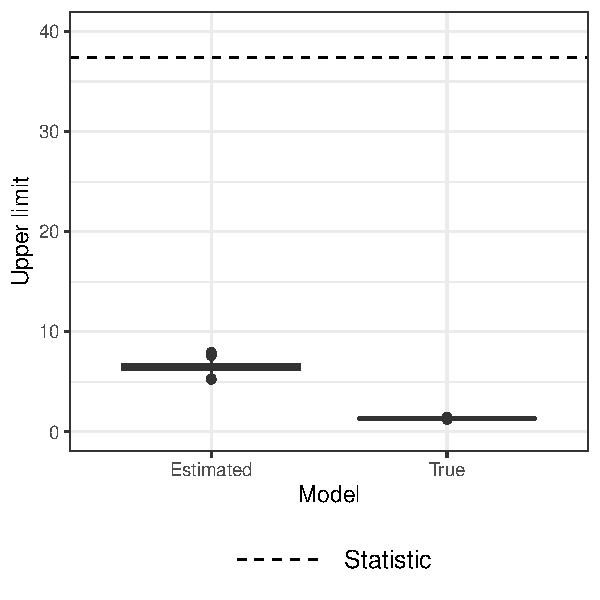
\includegraphics[width=\textwidth]{img/mcssa_ci_025.pdf}
		\caption{$\omega=0.25$}
		\label{fig:mcssa_ci_1}
	\end{subfigure}
	\begin{subfigure}{0.45\textwidth}
		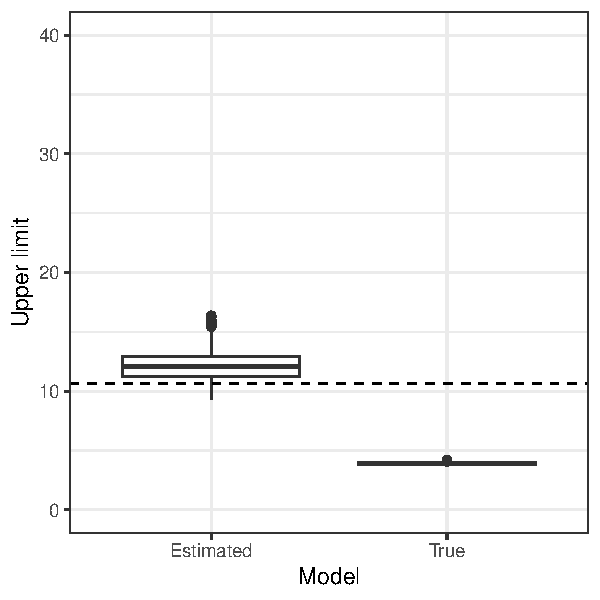
\includegraphics[width=\textwidth]{img/mcssa_ci_0125.pdf}
		\caption{$\omega=0.125$}
		\label{fig:mcssa_ci_2}
	\end{subfigure}
	\caption{Пример~\ref{eg:composite_signal}: верхние границы предсказательных интервалов}
	\label{fig:mcssa_ci}
\end{figure}

На рис.~\ref{fig:mcssa_ci} представлены распределение $\mu_k + q\sigma_k$ для величины $p_k$, соответствующей частоте $\omega=1/4=0.25$ (рис.~\ref{fig:mcssa_ci_1}) и соответствующей частоте $\omega=1/8=0.125$ (рис.~\ref{fig:mcssa_ci_2}), на каждом графике пунктирной линией обозначено значение статистики критерия $\widehat p_k$ (точнее его среднее значение). Как видим, в случае истинной модели шума обе частоты являются значимыми всегда. Когда параметры шума оцениваются, более сильная часть сигнала ($\omega=0.25$) все еще значима, в то время как более слабая часть ($\omega=0.125$) перестает быть значимой в большинстве случаев. То есть можно заметить значительное падение мощности критерия против альтернативы <<сигнал с частотой $\omega=0.125$>>. Связано это с консервативностью критерия при оценке параметров шума (см. раздел~\ref{sect:mcssa_est_model}).

\subsection{Оценка максимально значимой частоты}

Поскольку при непопадании частоты $\omega$ в решетку $k/(2L)$ оценка будет смещена, предлагаем следующую эвристику.

\begin{algorithm}[H]
	\caption{Оценка максимально значимой частоты с помощью MC-SSA}\label{alg:signif_freq_est}
	\Input статистики критерия $\widehat{p}_k$, $k=1,\ldots,L$.\\
	\Output максимально значимая частота $\omega^\star$.

	\begin{algorithmic}[1]
		\State Найти индекс наиболее значимой частоты: $k=\operatorname*{argmax}\limits_i \widehat{p}_i / c_i$, где $c_i$~--- верхняя граница доверительного интервала для $\widehat{p}_i$;
		\State Вычислить значение $\omega^\star$ как взвешенное среднее частот $\omega_{k-1}, \omega_k,\omega_{k+1}$ с весами $w_i=\max(0, \widehat{p}_i-c_i)$;
	\end{algorithmic}
\end{algorithm}

\subsection{Алгоритм}

Как было показано в разделе~\ref{sect:composite_signal_power}, при оцененных параметрах шума метод MC-SSA может обнаружить не все частоты, принадлежащие сигналу. Поэтому будем оценивать сигнал последовательно, применяя критерий MC-SSA к остатку до тех пор, пока гипотеза $H_0:\tS=0$ не перестанет отвергаться. Так на каждой итерации алгоритма определяется максимально значимая частота и применяется алгоритм~\ref{alg:auto_periodic}. С каждым шагом алгоритма оценка параметров шума становится точнее, тем самым критерий становится менее консервативным и более мощным. Стоит отметить, что, поскольку первая проверка гипотезы предлагаемого алгоритма совпадает с одним применением критерия MC-SSA, критерий остается точным для истинной модели шума и консервативным для оцененной (см. раздел~\ref{sect:mcssa_est_model}). Приведем в алгоритме~\ref{alg:autoMCSSA} алгоритм автоматической идентификации периодических компонент с помощью критерия MC-SSA, который назовем autoMCSSA. На рис.~\ref{fig:autoMCSSA_flowchart} изображена его упрощенная блок-схема.

\begin{algorithm}[!ht]
	\caption{autoMCSSA}
	\label{alg:autoMCSSA}
	\Input временной ряд $\tX$, элементарные восстановленные компоненты $\tX^{(j)}$, $j\in J$, длина окна $L\in(1, N)$, модель шума $\bm\xi$, уровень значимости $\alpha$, порог низких частот $\omega_0$, радиус $\delta \geqslant 0$, порог $T_0\in[0, 1]$.\\
	\Output индексы периодических компонент $J_\text{Periodics}$, оценка периодик $\hat \tP$.
	\begin{algorithmic}[1]
		\State Инициализируем оценку периодик $\hat\tP$ нулевым рядом, множество индексов $J_\text{Periodics} \coloneq \varnothing$ и диапазоны нерассматриваемых частот $\mathcal{B} \coloneq [0, \omega_0]$.
		\State Применить алгоритм~\ref{alg:multiple_mc-ssa_part_spectrum} к ряду $\tX$. Если нулевая гипотеза не отвергается при уровне значимости $\alpha$, завершить работу алгоритма.
		\State Пока $|J|\ne0$:
		\begin{algsubstates}
			\State Вычислить оценку максимально значимой частоты $\omega^\star$ (алгоритм~\ref{alg:signif_freq_est}).
			\State Получить компоненты $J_{\omega^\star}$ и оценку периодики $\tP_{\omega^\star}$ с помощью алгоритма~\ref{alg:auto_periodic} с рядами $\left\{\tX^{(j)}\right\}_{j\in J}$ и $d=d_{\cos}(\omega^\star)$~\eqref{eq:d_cos}.
			\State $J_\text{Periodics} \coloneq J_\text{Periodics}\cup J_{\omega^\star}$, $\hat{\tP} \coloneq \hat{\tP} + \tP_{\omega^\star}$, $\hat{\tN} \coloneq \tX - \hat{\tP}$.
			\State Если $|J_{\omega^\star}|=0$, $\mathcal{B} \coloneq \mathcal{B}\cup\left[\omega^\star - \delta, \omega^\star + \delta\right]$.
			\State \label{alg:auto_periodic_trend_modified_3} Применить к остатку $\hat{\tN}$ алгоритм~\ref{alg:multiple_mc-ssa_part_spectrum}. Если гипотеза не отвергается при уровне значимости $\alpha$, завершить работу алгоритма.
			\State $J \coloneq J \setminus J_{\omega^\star}$.
		\end{algsubstates}
	\end{algorithmic}
\end{algorithm}

\begin{figure}[htbp]
	\centering
	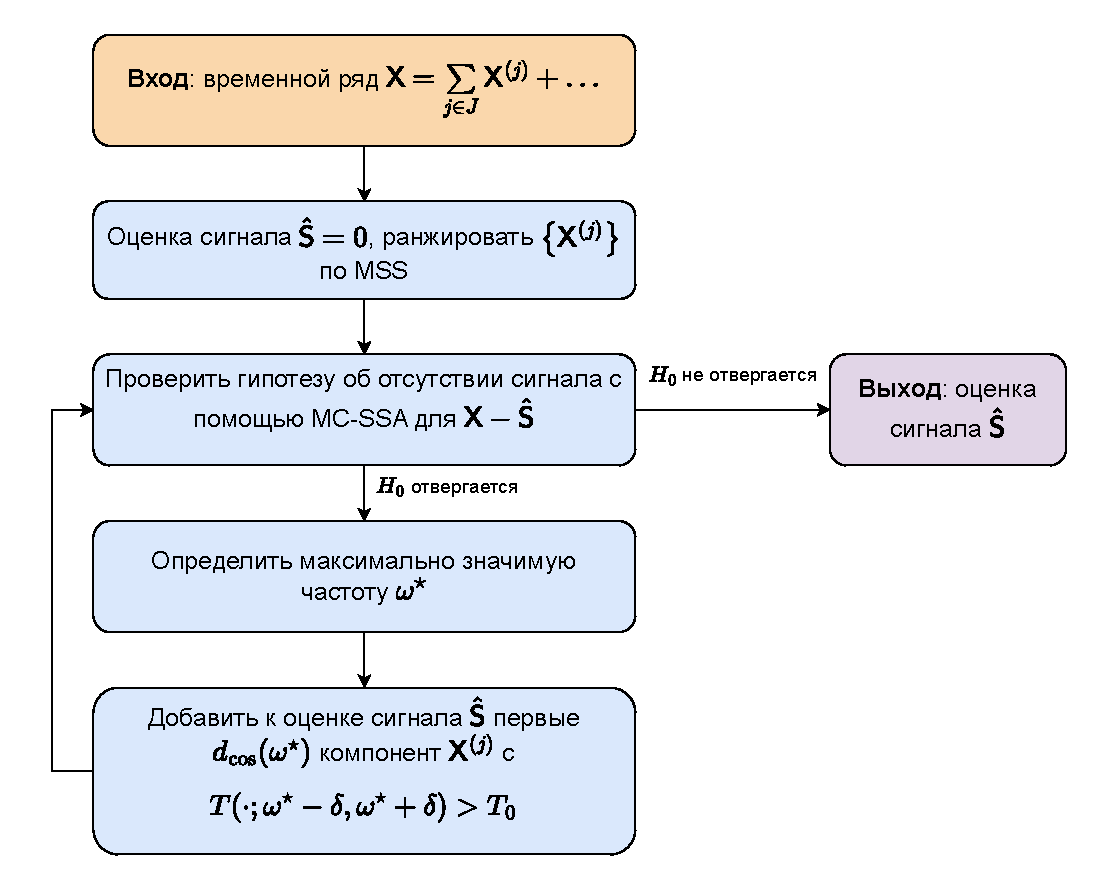
\includegraphics[width=0.85\textwidth]{img/auto_mcssa_flowchart.pdf}
	\caption{Блок-схема метода autoMCSSA}
	\label{fig:autoMCSSA_flowchart}
\end{figure}

\subsection{Пример работы алгоритма}\label{sect:autoMCSSA_example}

Рассмотрим пример работы autoMCSSA. Пусть $\mathsf{X}=\mathsf{S}+\bm{\xi}$, где $\bm\xi$~--- красный шум с параметрами $\phi=0.7$ и $\sigma^2=1$, $N=200$, $\mathsf{S}=(s_1,\ldots, s_N)$,
\[
	s_n=0.075\, e^{0.02n}\cos(2\pi n/8) + \cos(2\pi n / 4) + 0.2\cdot(-1)^n.
\]

\begin{figure}[!h]
	\centering
	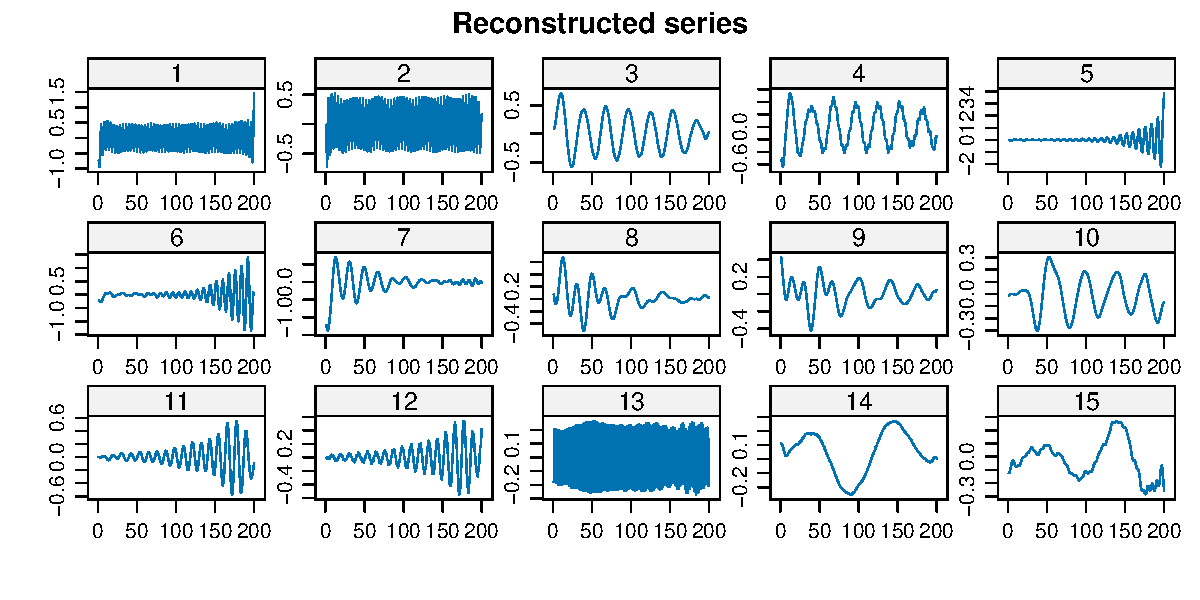
\includegraphics[width=0.8\textwidth]{img/reconstructed_ts.pdf}
	\caption{Элементарные восстановленные компоненты}
	\label{fig:reconstructed_ts}
\end{figure}

\begin{figure}[!h]
	\centering
	
\includegraphics[width=0.8\textwidth]{img/auto_mcssa_result.pdf}
	\caption{Результат autoMCSSA ($L=48$, $\delta=1/80$, $T_0=0.5$)}
	\label{fig:autoMCSSA_res}
\end{figure}

На рис.~\ref{fig:reconstructed_ts} представлены первые $15$ элементарных восстановленных  с помощью SSA компонент (длина окна $L_\text{SSA}=96$). Сигналу соответствуют компоненты с индексами $1$, $2$, $5$, $6$ и $13$. Не видя формулы, по которой этот сигнал задается, сказать наверняка, какие компоненты неслучайные, проблематично, поскольку компоненты ($3, 4$) и ($11, 12$) похожи на пары гармоник. Получено, что разработанный метод правильно идентифицировал компоненты, соответствующие сигналу, на рис.~\ref{fig:autoMCSSA_res} представлены истинная форма сигнала $\mathsf{S}$ и его оценка методом autoMCSSA.

\begin{remark}
	Для демонстрации работы алгоритма параметры $\delta$ и $T_0$ были подобраны так, чтобы autoMCSSA выделил весь сигнал. В общем случае выбор оптимальных $\delta$ и $T_0$ проблематичен. Эта проблема будет исследована далее в разделе~\ref{sect:autoMCSSA_opt_param}.
\end{remark}

\subsection{Выбор оптимальных параметров}\label{sect:autoMCSSA_opt_param}

Частота экспоненциально-модулированной гармоники~\eqref{eq:em_harmonic}, в отличие от гармоники с постоянной амплитудой, всегда растекается по спектру. Чем больше абсолютное значение показателя экспоненты $a$, тем сильнее это растекание. Поэтому радиус частотного интервала $\delta$ должен зависеть от величины $|a|$. Из формулы~\eqref{eq:em_harmonic} видно, что амплитуда сигнала в точке $N$ равна $e^{aN}$, поэтому можно считать, что $C=aN$~--- величина амплитудной модуляции.

Пусть $\tilde \Pi(k / N) = \Pi(k / N) / \sum_{k} \Pi(k / N)$~--- нормированная (односторонняя) периодограмма, где $\Pi(k / N)$ определена в формуле~\eqref{eq:pgram_corrected}. Обозначим за $\tilde\Pi^{C, \omega}$ нормированную периодограмму для сигнала с частотой $\omega$ и амплитудной модуляцией $C$. Отсортируем частоты $k/N$ по убыванию расстояния до частоты $\omega$, обозначим их как $\omega_{(n)}$, $n=0,\ldots,\lfloor N/2\rfloor$.
Рассмотрим следующие $\delta$:
\begin{equation}\label{eq:delta_n}
	\delta_{n}=|\omega_{(n)} - \omega|, \quad n=0,\ldots,\lfloor N/2\rfloor.
\end{equation}

% Обозначим $\delta_0=|\omega - \omega_{(2)}|$ (расстояние до дальней соседней точки), если $\omega$ не попадает в решетку периодограммы, иначе $\delta_0=0$. Рассмотрим следующие $\delta_n$:
% \begin{equation}\label{eq:delta_n}
% 	\delta_n=\delta_0 + n / N, \quad n=1,\ldots,\lfloor N / 2 \rfloor.
% \end{equation}
Введем частичные суммы вокруг главной частоты:
\begin{equation}\label{eq:Sigma_n}
	% \Sigma^{C, \omega}_n=\sum_{m:~|\omega_{(k)} - \omega| \leqslant \delta_{n}} \tilde\Pi^{C, \omega}\left(\omega_{(m)}\right), \quad n=0,\ldots,\lfloor N / 2 \rfloor.
	\Sigma^{C, \omega}_n=\sum_{m=0}^{n} \tilde\Pi^{C, \omega}\left(\omega_{(m)}\right), \quad n=0,\ldots,\lfloor N / 2 \rfloor.
\end{equation}
% Тогда рассмотрим следующий выбор $\delta$ в зависимости от частоты $\omega$ и силы модуляции $C$: находим такое первое $n=n^*$, что $\Sigma^{C, \omega}_{n^*} > \Sigma_t$ и $\delta_{n^*}>0$, и берем $\delta = \delta_{n^*} \eqcolon \delta^*$. То есть выбираем такое $\delta$, чтобы захватывать б\'{о}льшую часть спектра.
Тогда рассмотрим следующий выбор $\delta$ в зависимости от частоты $\omega$ и силы модуляции $C$: находим такое первое $n=n^*$, что $\Sigma^{C, \omega}_{n^*} > \Sigma_t$ и $\delta_{n^*}>0$ и берем $\delta = \delta_{n^*} \eqcolon \delta^*$. То есть выбираем такое $\delta$, чтобы захватывать б\'{о}льшую часть спектра.

\begin{figure}[h!]
	\centering
	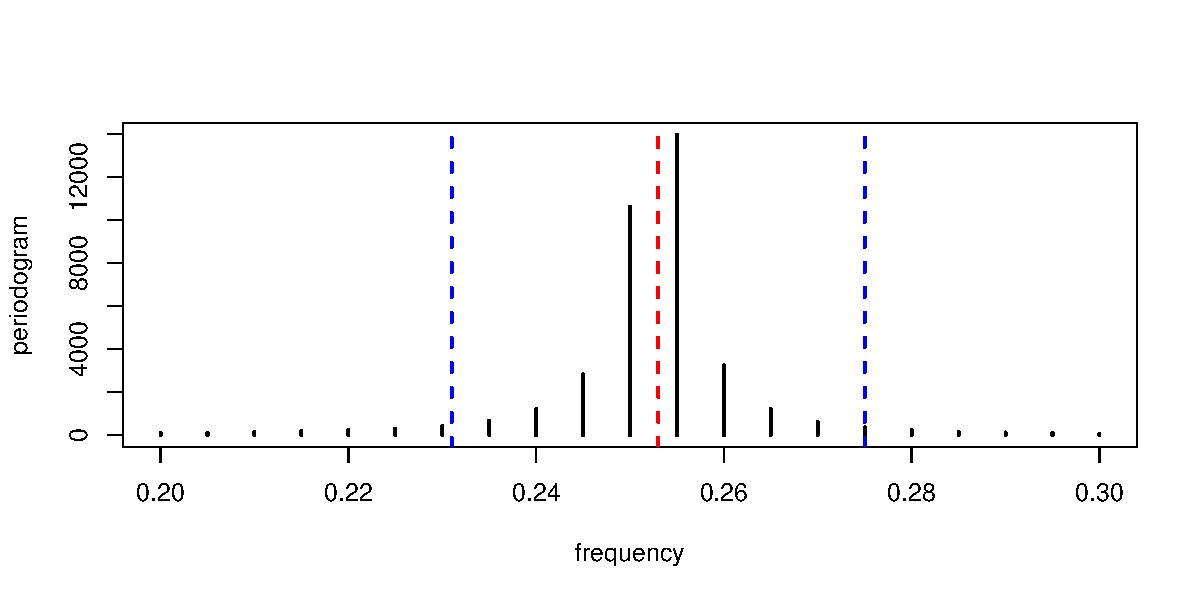
\includegraphics[width=\linewidth]{img/delta_choice_example.pdf}
	\caption{Границы частотного интервала при $\delta=\delta^*$ ($N=200$, $C=4$, $\omega=0.253$, $\Sigma_t=0.9$)}
	\label{fig:delta_choice_example}
\end{figure}

Рассмотрим пример. Пусть $N=200$, $C=4$, $\omega=0.253$. На рис.~\ref{fig:delta_choice_example} изображена периодограмма такого сигнала, красной пунктирной линией обозначена главная частота.
%Одним цветом покрашены значения $\Sigma^{C, \omega}_n - \Sigma^{C, \omega}_{n-1}$, то есть при переходе от $n$ к $n+1$ количество частот, участвующих в сумме, увеличивается на $2$.
Пусть $\Sigma_t=0.9$, тогда $\delta^*=0.022$, границы частотного интервала обозначены на графике синими пунктирными линиями.

Для проверки, насколько такой выбор $\delta$ оптимален, сравним его с другим (итеративным) подходом к выбору $\delta$: будем увеличивать $n$ до тех пор, пока для $\delta=\delta_{n}$ не обнаружится $d_{\cos}(\omega)$~\eqref{eq:d_cos} компонент.

\subsubsection{Численное сравнение}\label{sect:delta_choice_numerical_research}

Проведем численный эксперимент и посчитаем ошибку восстановления сигнала для обоих способов выбора $\delta$. Не ограничивая общности, будем считать, что $C\geqslant0$, поскольку форма периодограммы для $C$ и $-C$ совпадают. Для исследования были выбраны следующие $C$: $0$ (отсутствие модуляции), $1$ (слабая модуляция), $2$ (умеренная модуляция), $5$ (сильная модуляция). Учитывая, что, помимо $\delta$, существует параметр $T_0$ (см. алгоритм~\ref{alg:auto_periodic}), выбор которого тоже затруднителен, рассмотрим сетку из возможных значений порога.

Пусть $N=200$, $\omega=0.25$. Параметры шума $\phi=0.7$, $\sigma^2=4$. Амплитуды $A$ для гармоник выбирать будем так, чтобы их SNR по формуле~\eqref{eq:snr} совпадали и равнялись $0.25$. Для вычисления $\delta^*$ рассмотрим $\Sigma_t=0.9$.

\begin{remark}
	Поскольку основное преимущество autoMCSSA~--- умение выделять сигнал с недоминирующими компонентами, частота сигнала и дисперсия белого шума были выбраны так, чтобы сигнал был отделим от шума и чтобы компоненты сигнала в SSA не были доминирующими. Далее в примерах будет рассмотрен сигнал с меньшей частотой, однако стоит учитывать, что в таком случае при корректировке SNR компоненты сигнала выйдут на первые позиции из-за вида спектральной плотности красного шума (убывающая функция).
\end{remark}

\begin{figure}[!h]
	\centering
	\begin{subfigure}{0.45\textwidth}
		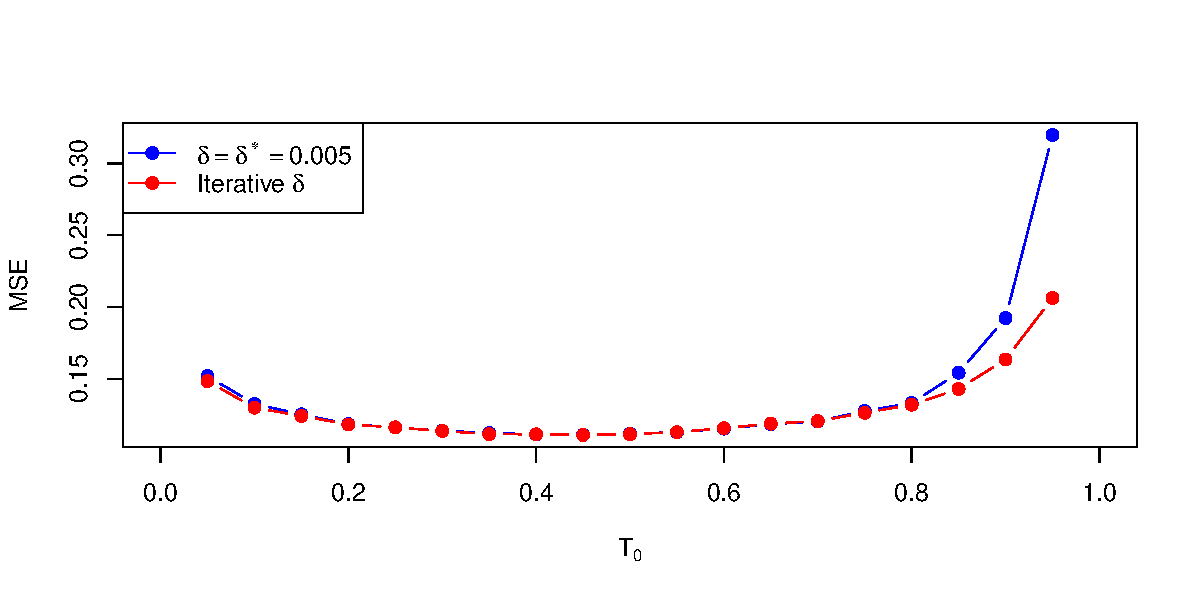
\includegraphics[width=\textwidth]{img/mse_omega025_C0.pdf}
		\caption{$C=0$}
	\end{subfigure}
	\begin{subfigure}{0.45\textwidth}
		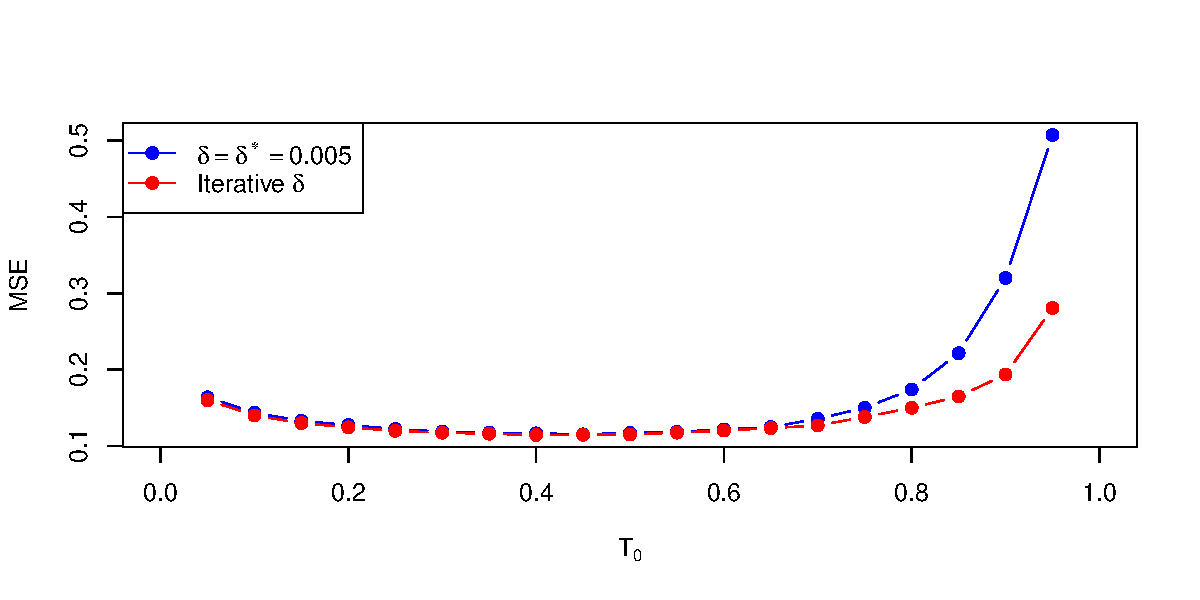
\includegraphics[width=\textwidth]{img/mse_omega025_C1.pdf}
		\caption{$C=1$}
	\end{subfigure}
	\begin{subfigure}{0.45\textwidth}
		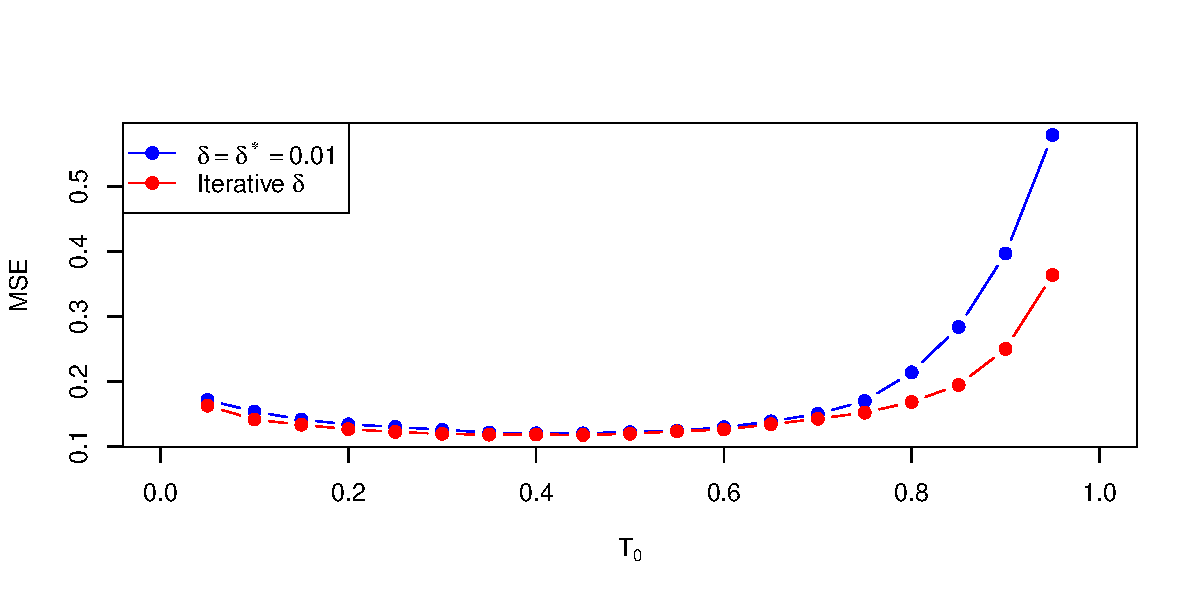
\includegraphics[width=\textwidth]{img/mse_omega025_C2.pdf}
		\caption{$C=2$}
	\end{subfigure}
	\begin{subfigure}{0.45\textwidth}
		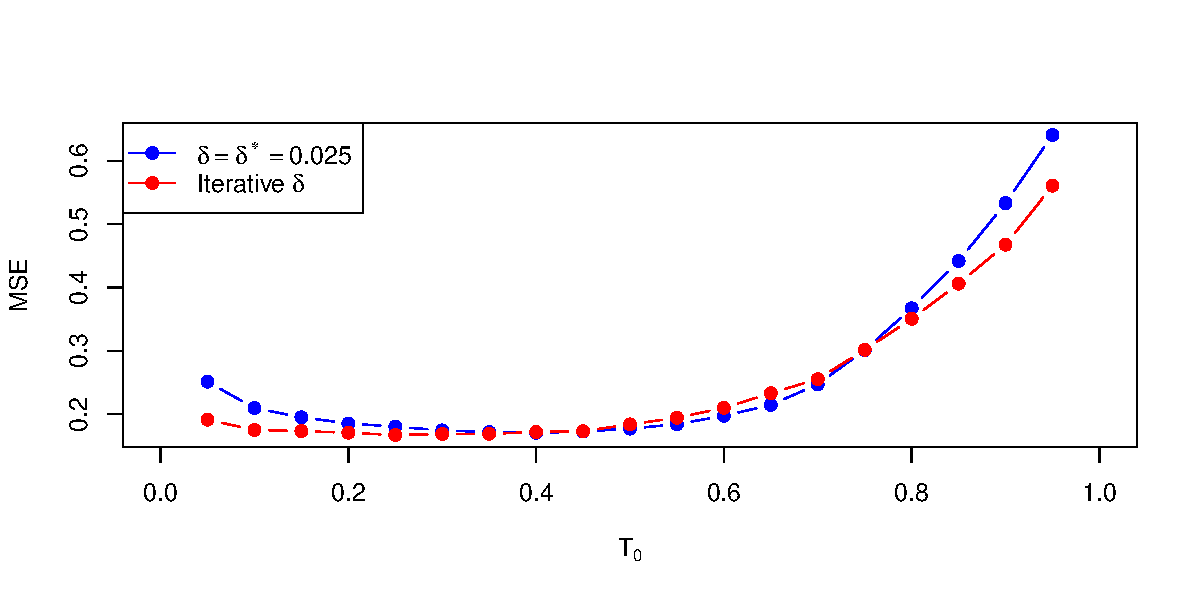
\includegraphics[width=\textwidth]{img/mse_omega025_C5.pdf}
		\caption{$C=5$}
	\end{subfigure}
	\caption{Ошибка восстановления сигнала для разных $C$ и $T_0$ ($\omega=0.25$)}
	\label{fig:mse_omega025}
\end{figure}

\begin{figure}[!h]
	\centering
	\begin{subfigure}{0.45\textwidth}
		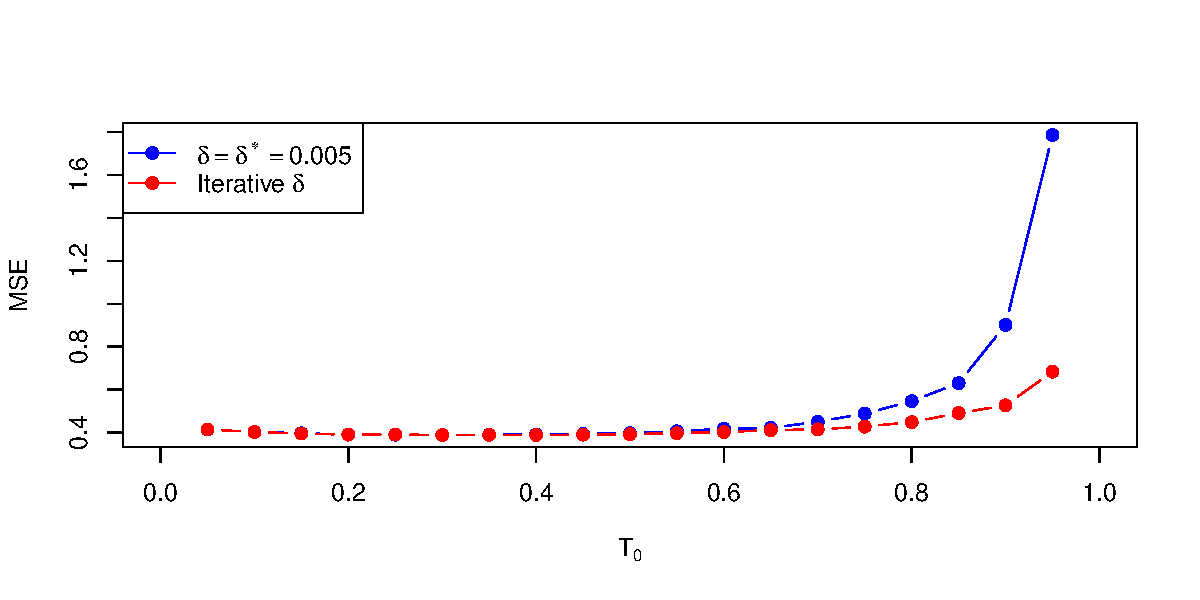
\includegraphics[width=\textwidth]{img/mse_omega01_C0.pdf}
		\caption{$C=0$}
	\end{subfigure}
	\begin{subfigure}{0.45\textwidth}
		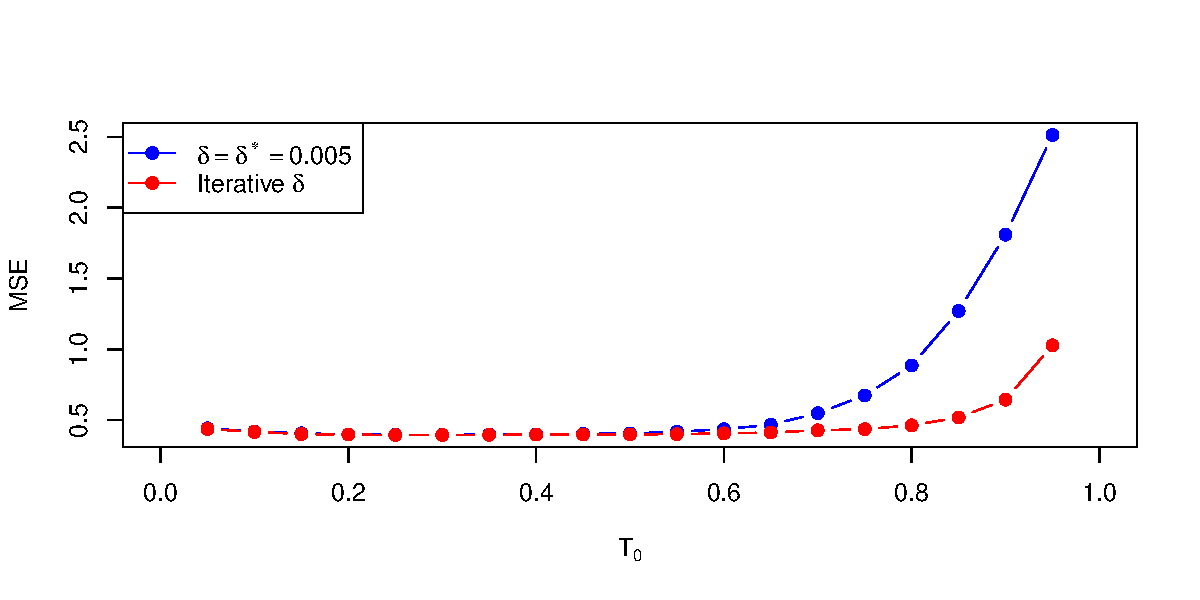
\includegraphics[width=\textwidth]{img/mse_omega01_C1.pdf}
		\caption{$C=1$}
	\end{subfigure}
	\begin{subfigure}{0.45\textwidth}
		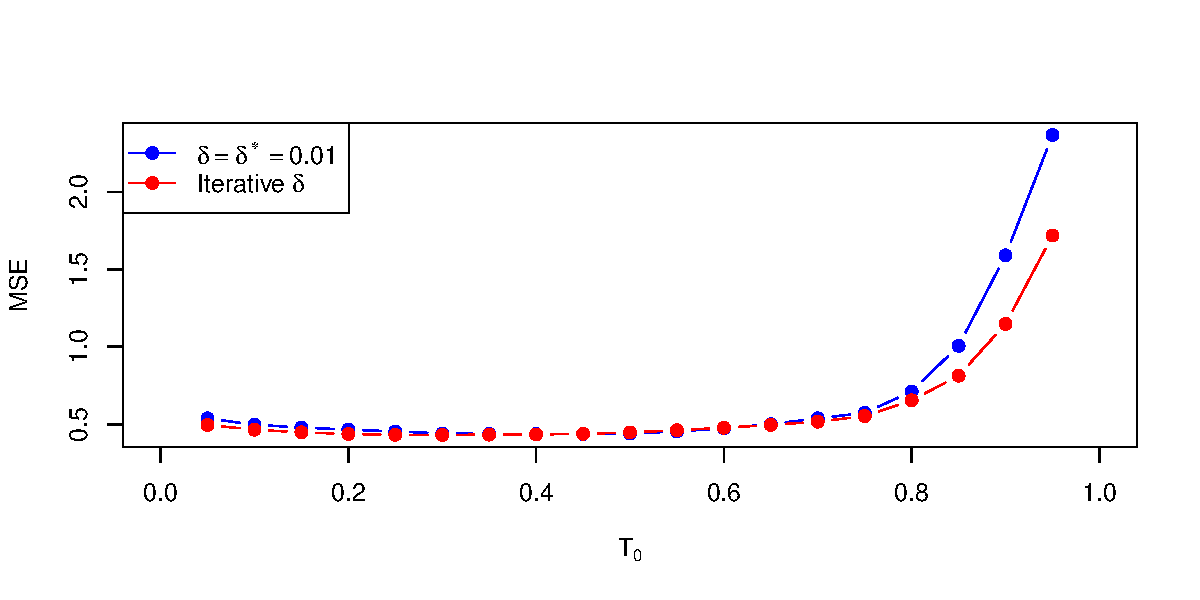
\includegraphics[width=\textwidth]{img/mse_omega01_C2.pdf}
		\caption{$C=2$}
	\end{subfigure}
	\begin{subfigure}{0.45\textwidth}
		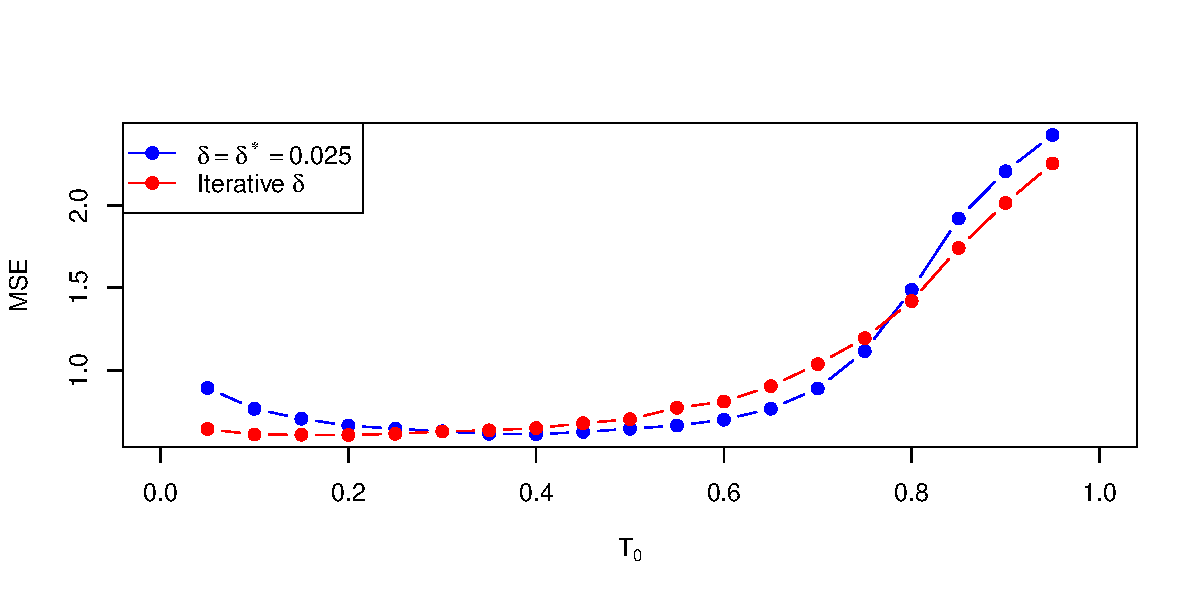
\includegraphics[width=\textwidth]{img/mse_omega01_C5.pdf}
		\caption{$C=5$}
	\end{subfigure}
	\caption{Ошибка восстановления сигнала для разных $C$ и $T_0$ ($\omega=0.1$)}
	\label{fig:mse_omega01}
\end{figure}

На рис.~\ref{fig:mse_omega025} представлены MSE восстановления сигнала для двух подходов к выбору $\delta$ для разных значений порога $T_0$. Стоит отметить следующую зависимость ошибки от порога: при увеличении $T_0$ ошибки сначала уменьшаются, достигая минимума, а затем увеличиваются. Для $\delta=\delta^*$ этот минимум находится в интервале $[0.4, 0.5]$, но разница в ошибках внутри этого интервала незначительна. Можно заметить, что для $C\geqslant2$ графики для $\delta=\delta^*$ и итеративного $\delta$ практически совпадают, за исключением больших значений порога. Для сильной модуляции итеративный вариант дает меньшую ошибку для малых значений $T_0$, но наименьшее значение MSE примерно такое же, что и у первого варианта.

\begin{figure}[!h]
	\centering
	\begin{subfigure}{0.45\textwidth}
		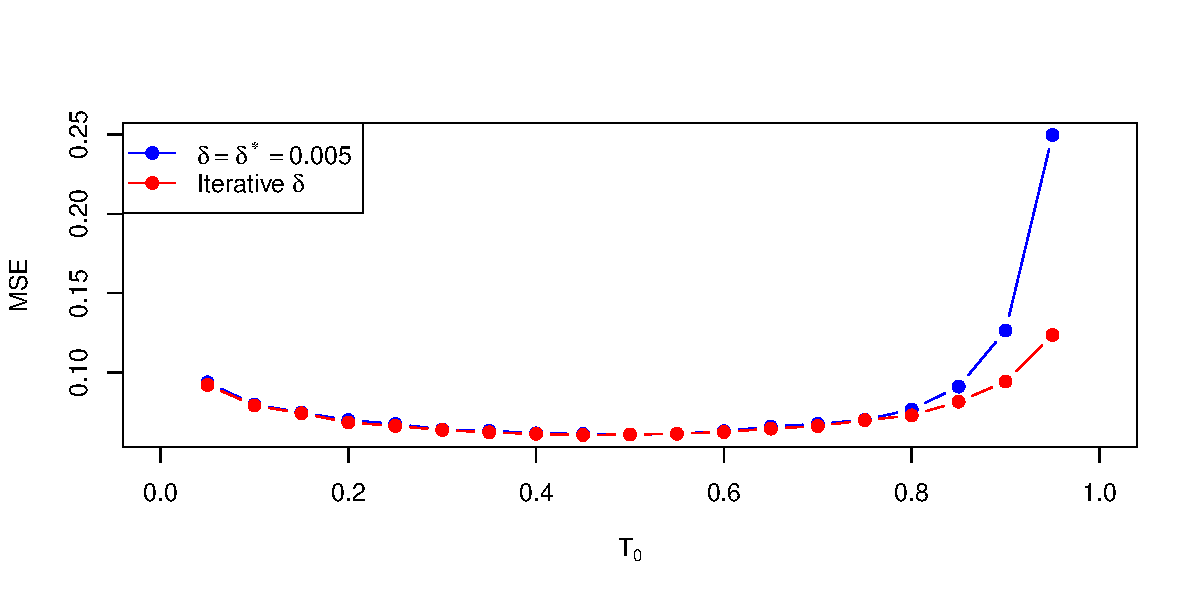
\includegraphics[width=\textwidth]{img/mse_omega04_C0.pdf}
		\caption{$C=0$}
	\end{subfigure}
	\begin{subfigure}{0.45\textwidth}
		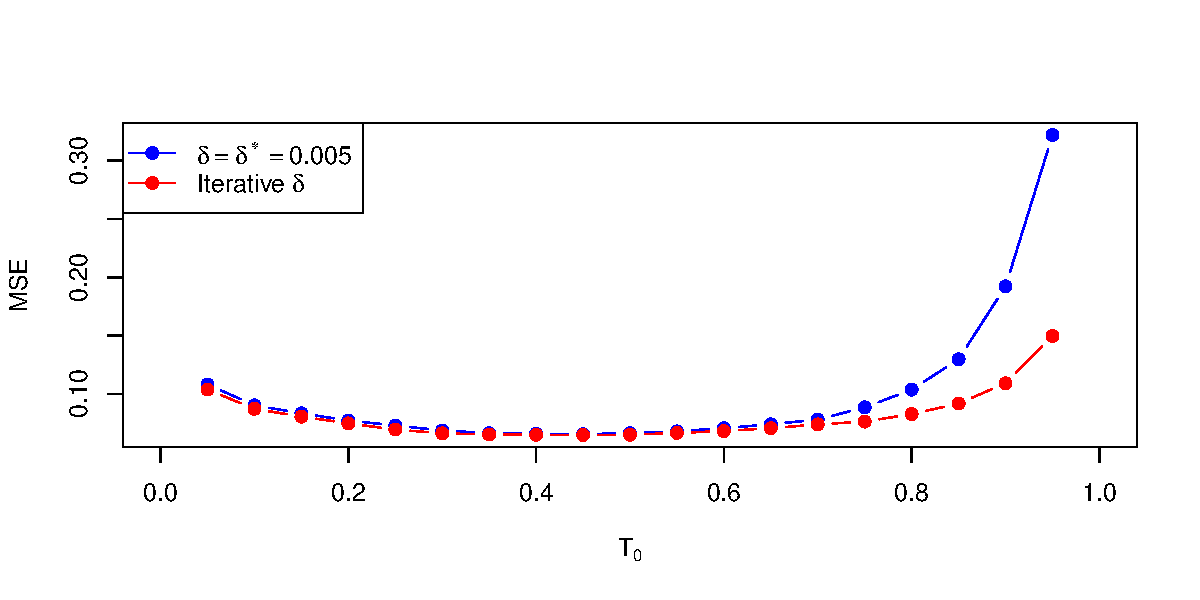
\includegraphics[width=\textwidth]{img/mse_omega04_C1.pdf}
		\caption{$C=1$}
	\end{subfigure}
	\begin{subfigure}{0.45\textwidth}
		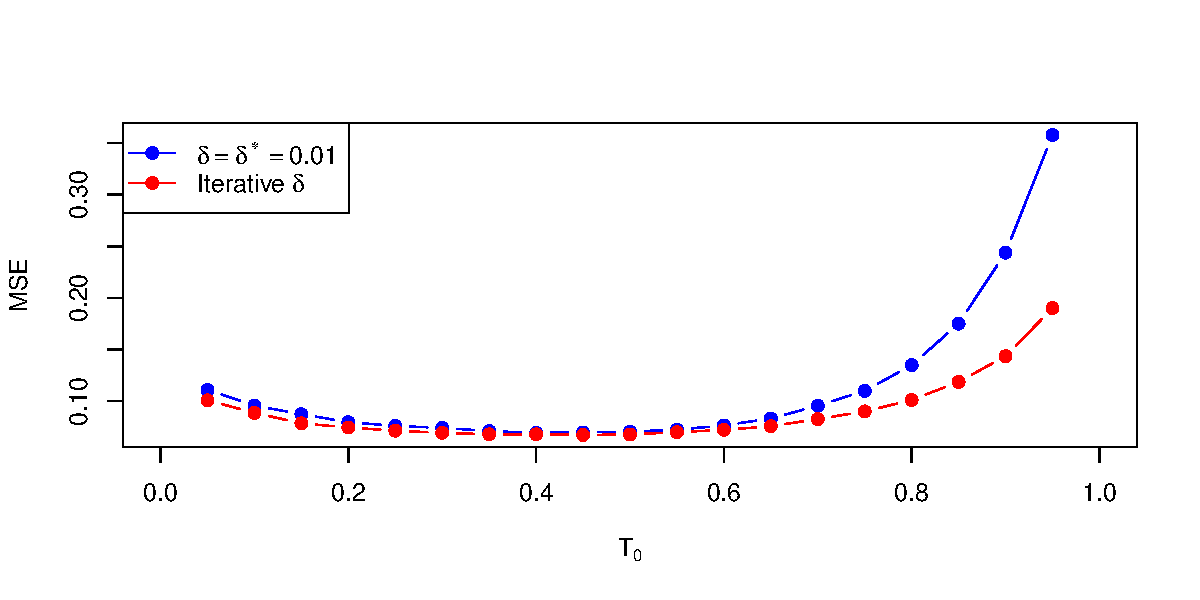
\includegraphics[width=\textwidth]{img/mse_omega04_C2.pdf}
		\caption{$C=2$}
	\end{subfigure}
	\begin{subfigure}{0.45\textwidth}
		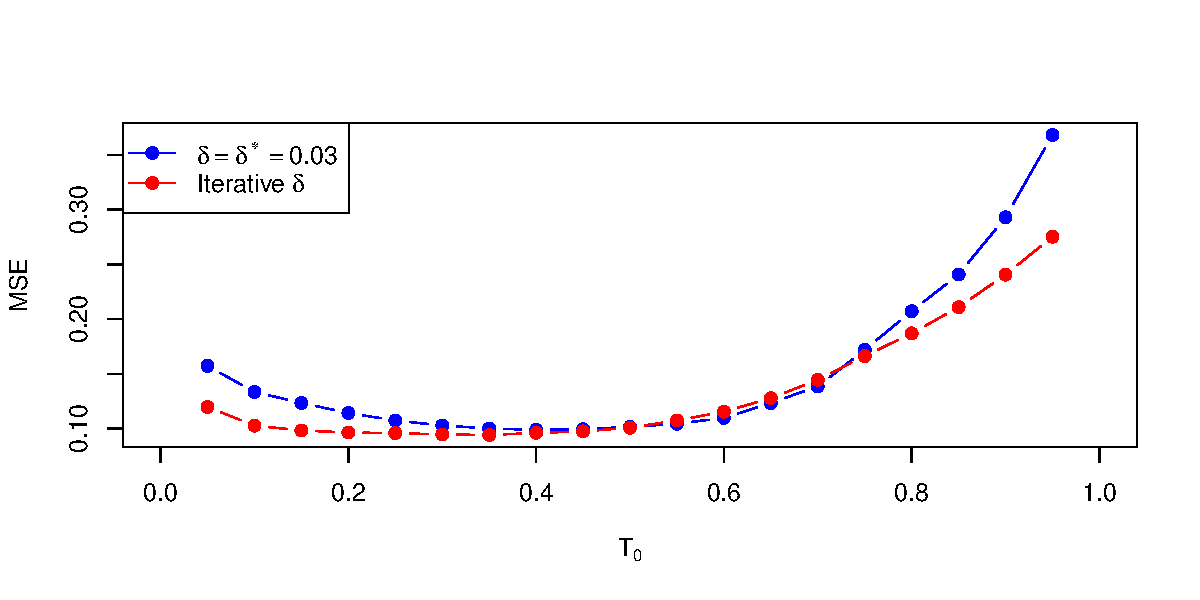
\includegraphics[width=\textwidth]{img/mse_omega04_C5.pdf}
		\caption{$C=5$}
	\end{subfigure}
	\caption{Ошибка восстановления сигнала для разных $C$ и $T_0$ ($\omega=0.4$)}
	\label{fig:mse_omega04}
\end{figure}

\begin{figure}[!h]
	\centering
	\begin{subfigure}{0.45\textwidth}
		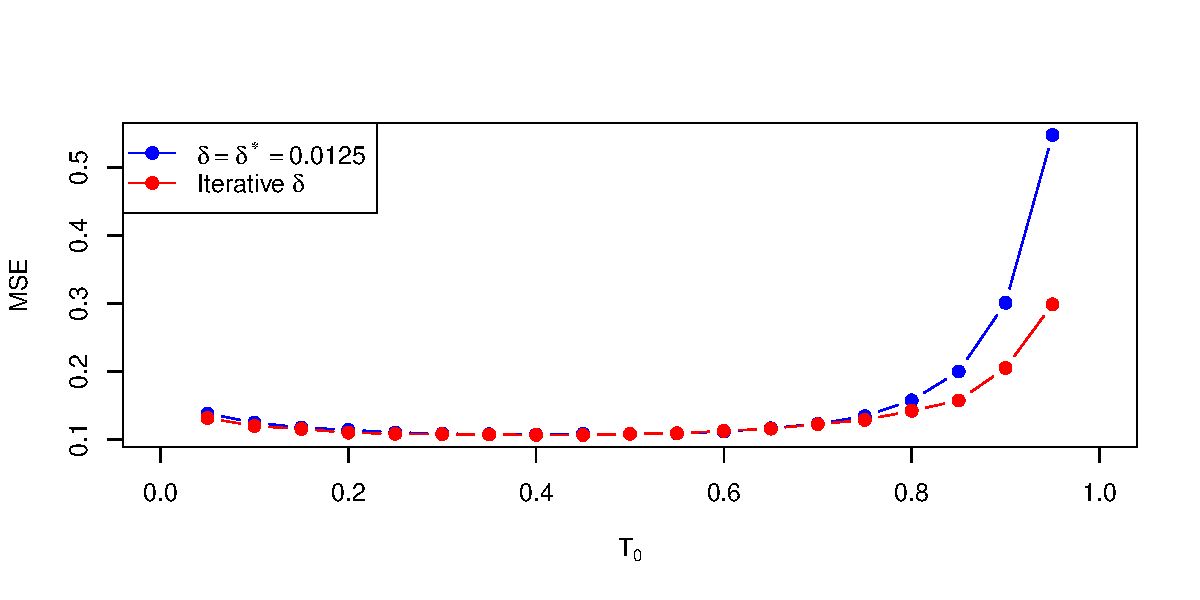
\includegraphics[width=\textwidth]{img/mse_omega02525_C0.pdf}
		\caption{$C=0$}
	\end{subfigure}
	\begin{subfigure}{0.45\textwidth}
		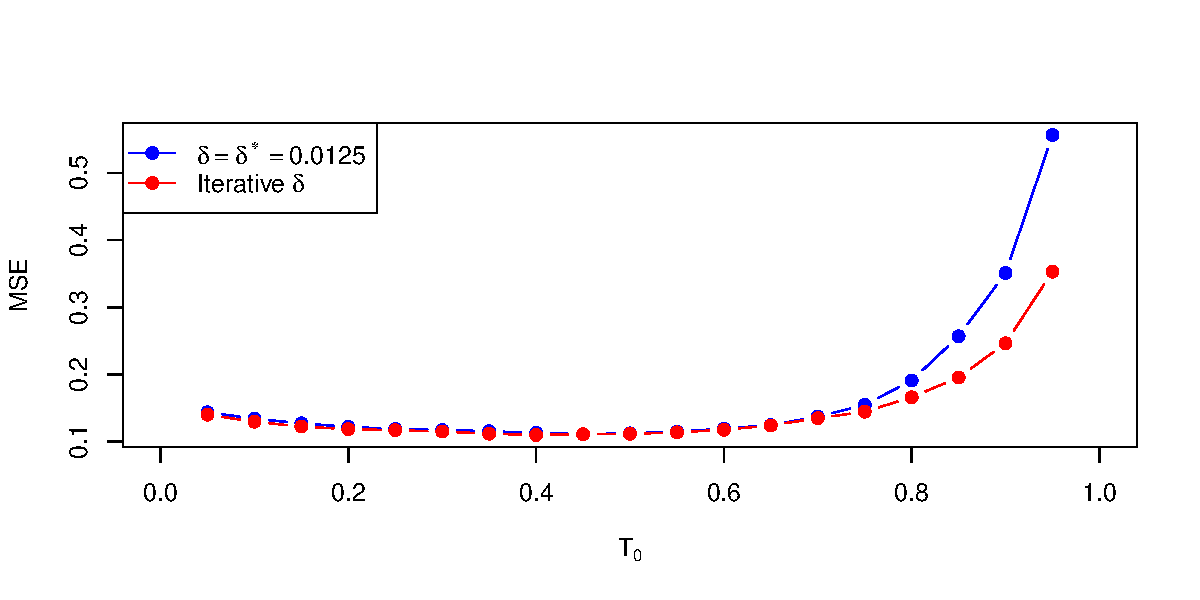
\includegraphics[width=\textwidth]{img/mse_omega02525_C1.pdf}
		\caption{$C=1$}
	\end{subfigure}
	\begin{subfigure}{0.45\textwidth}
		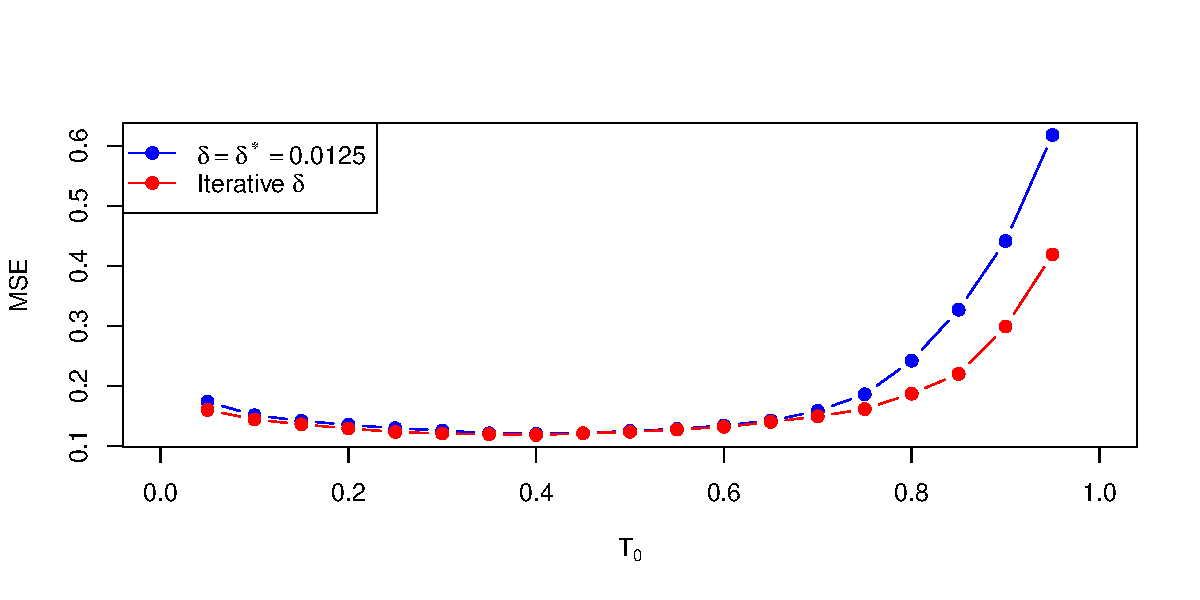
\includegraphics[width=\textwidth]{img/mse_omega02525_C2.pdf}
		\caption{$C=2$}
	\end{subfigure}
	\begin{subfigure}{0.45\textwidth}
		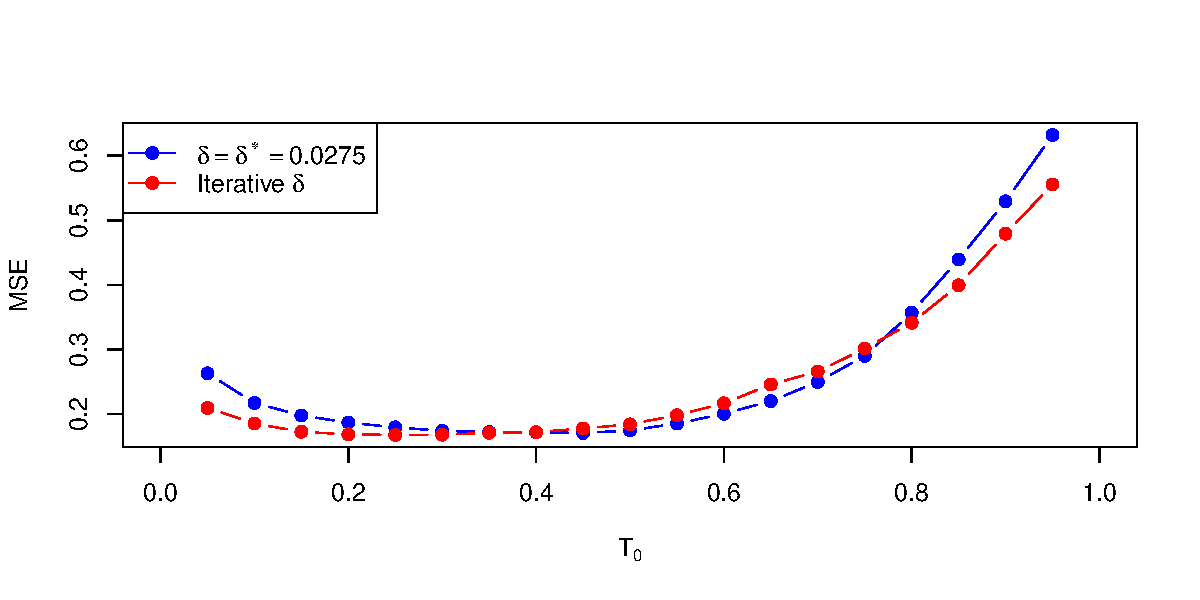
\includegraphics[width=\textwidth]{img/mse_omega02525_C5.pdf}
		\caption{$C=5$}
	\end{subfigure}
	\caption{Ошибка восстановления сигнала для разных $C$ и $T_0$ ($\omega=0.2525$)}
	\label{fig:mse_omega02525}
\end{figure}

Увеличим/уменьшим главную частоту сигнала и проверим, можно ли сделать те же выводы, что и в случае $\omega=0.25$. На рис.~\ref{fig:mse_omega01} и~\ref{fig:mse_omega04} представлены результаты для $\omega=0.1$ и $\omega=0.4$ соответственно. Как видим, поведение графиков практически идентично случаю $\omega=0.25$.

Теперь пусть частота не попадает в решетку периодограммы: $\omega=0.2525$ (наихудший случай, частота попала ровно посередине между частотами). Результаты моделирования представлены на рис.~\ref{fig:mse_omega02525}. Как видно, по данным графикам можно сделать аналогичные предыдущим случаям выводы.

По результатам численного исследования можно сделать следующие выводы:

\begin{enumerate}
	\item Оба способа выбора $\delta$ дают примерно одинаковую минимальную ошибку.
	\item Минимальная ошибка достигается при $T_0\in[0.4, 0.5]$.
\end{enumerate}

Учитывая это и некоторые вычислительные сложности итеративного метода, предпочтение отдается варианту с $\delta=\delta^*$.

\subsubsection{Случай неизвестной амплитудной модуляции}\label{sect:C_max}

В предыдущем разделе предполагалось, что истинная модуляция $C$ известна, что, конечно же, не верно на практике. Поэтому можно допустить максимально возможную (но не слишком большую) в ряде модуляцию $C_{\max}$ и брать $\delta=\delta^*(\omega, C_{\max})$.

\begin{figure}[!h]
	\centering
	\begin{subfigure}{0.3\textwidth}
		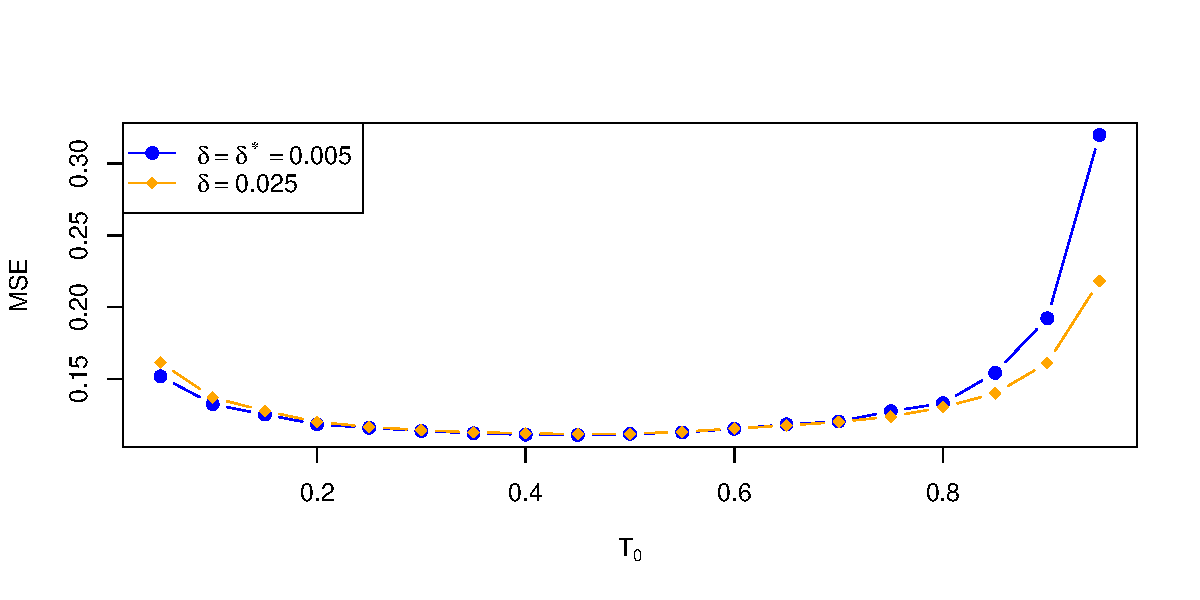
\includegraphics[width=\textwidth]{img/mse_omega025_Cmax_0.pdf}
		\caption{$C=0$}
	\end{subfigure}
	\begin{subfigure}{0.3\textwidth}
		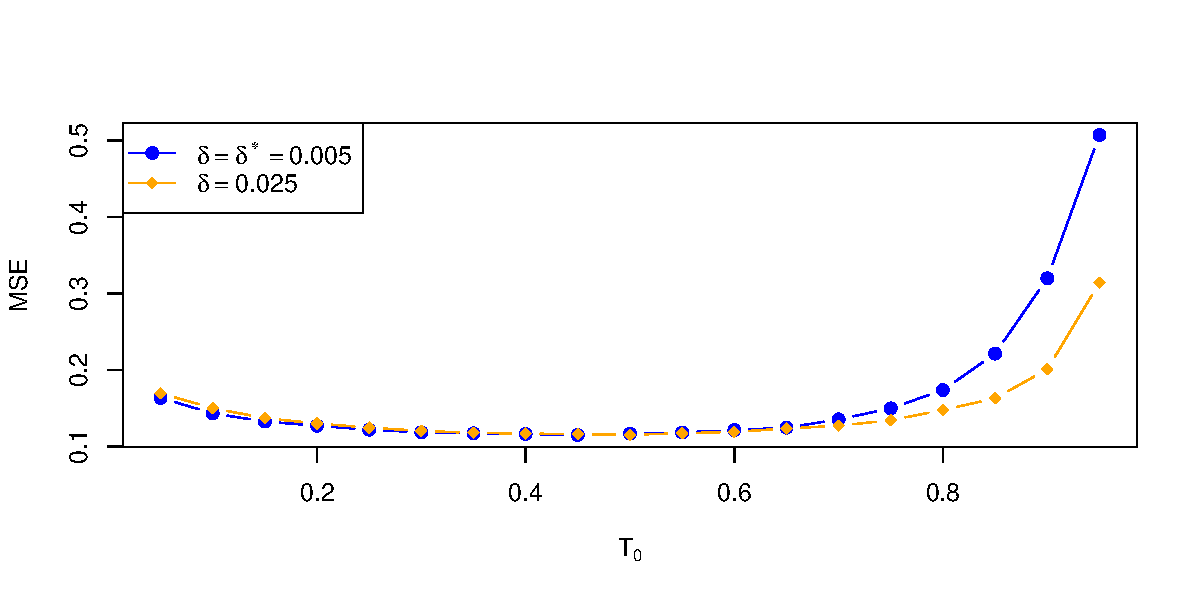
\includegraphics[width=\textwidth]{img/mse_omega025_Cmax_1.pdf}
		\caption{$C=1$}
	\end{subfigure}
	\begin{subfigure}{0.3\textwidth}
		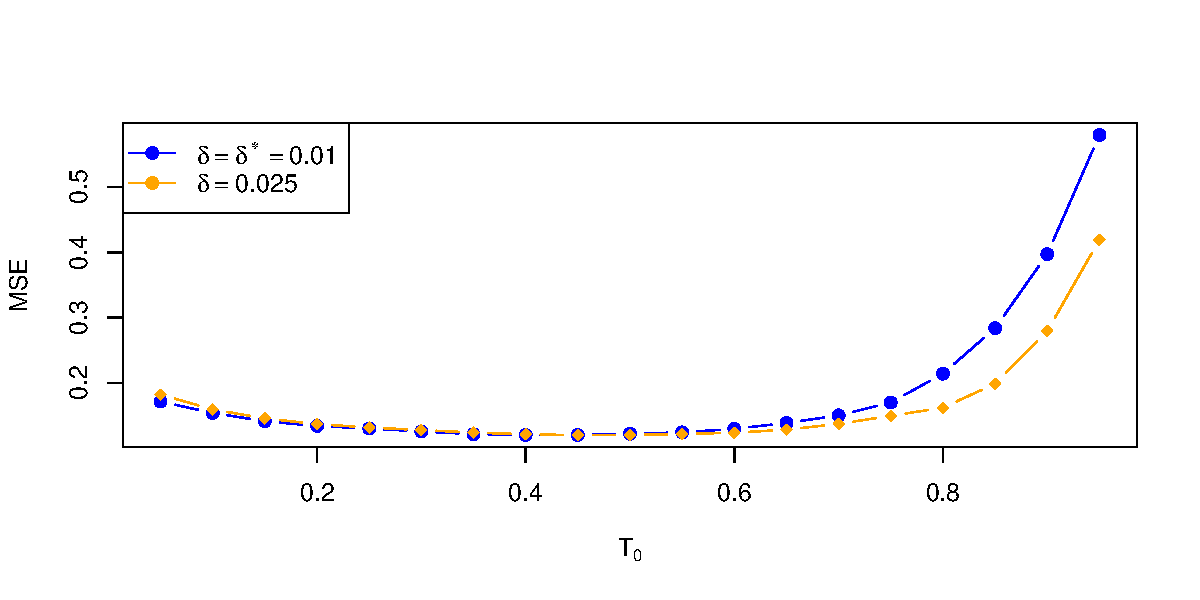
\includegraphics[width=\textwidth]{img/mse_omega025_Cmax_2.pdf}
		\caption{$C=2$}
	\end{subfigure}
	\caption{Ошибка восстановления сигнала для разных $C$ и $T_0$ ($\omega=0.25$, $C_{\max}=5$)}
	\label{fig:mse_omega025_Cmax}
\end{figure}

\begin{figure}[!h]
	\centering
	\begin{subfigure}{0.3\textwidth}
		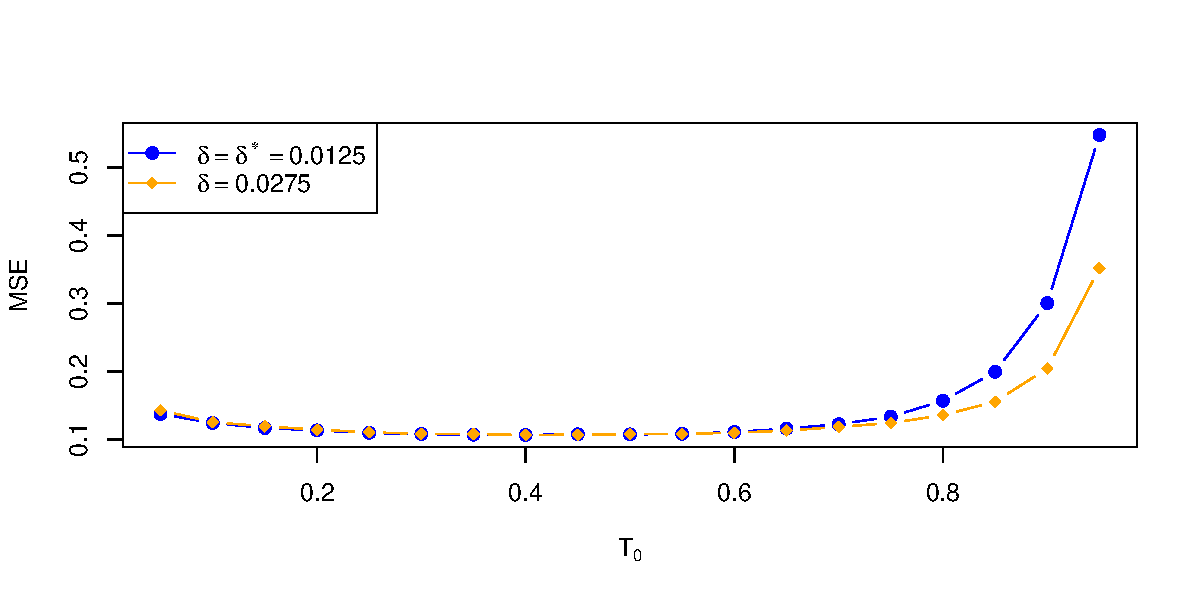
\includegraphics[width=\textwidth]{img/mse_omega02525_Cmax_0.pdf}
		\caption{$C=0$}
	\end{subfigure}
	\begin{subfigure}{0.3\textwidth}
		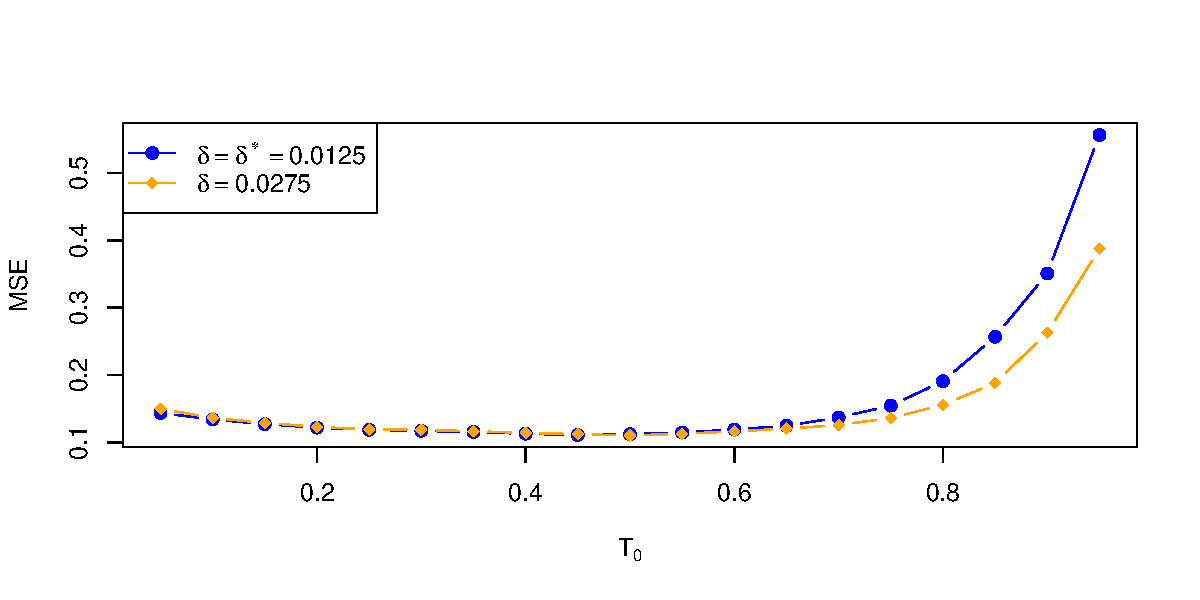
\includegraphics[width=\textwidth]{img/mse_omega02525_Cmax_1.pdf}
		\caption{$C=1$}
	\end{subfigure}
	\begin{subfigure}{0.3\textwidth}
		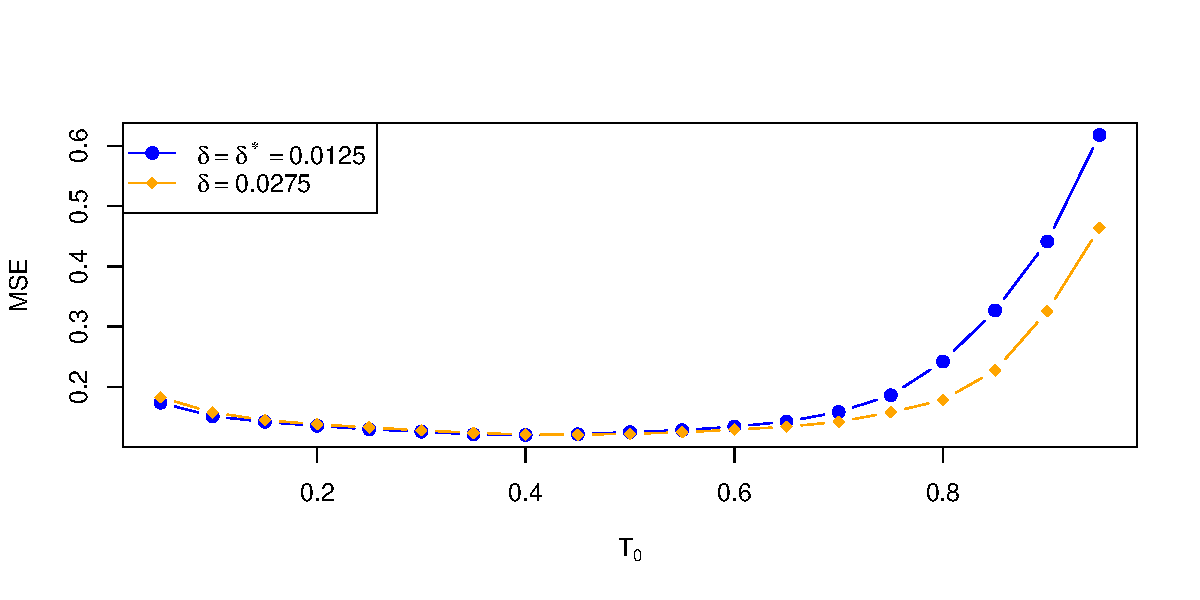
\includegraphics[width=\textwidth]{img/mse_omega02525_Cmax_2.pdf}
		\caption{$C=2$}
	\end{subfigure}
	\caption{Ошибка восстановления сигнала для разных $C$ и $T_0$ ($\omega=0.2525$, $C_{\max}=5$)}
	\label{fig:mse_omega02525_Cmax}
\end{figure}

Пусть $C_{\max}=5$, $\Sigma_t=0.9$. На примерах из раздела~\ref{sect:delta_choice_numerical_research} посмотрим на применимость данного подхода. На рис.~\ref{fig:mse_omega025_Cmax} и рис.~\ref{fig:mse_omega02525_Cmax} представлены результаты моделирования. Видно, что оптимальный порог $T_0$ совпадает со случаем истинного $C$. Можно сделать вывод, что выбор $\delta$ по верхней границе для амплитудной модуляции не портит оценку сигнала c $\delta=\delta^*$. Приведем в алгоритме~\ref{alg:delta_opt} результирующий алгоритм выбора радиуса $\delta$ при заданной границе $C_{\max}$.

\begin{algorithm}[!ht]
	\caption{Выбор радиуса частотного интервала при заданной границе величины амплитуднои модуляции}
	\label{alg:delta_opt}
	\Input Длина ряда $N$, частота $\omega$, верхняя граница величины амплитудной модуляции $C_{\max}$, порог $\Sigma_t$.\\
	\Output Радиус частотного интервала $\delta^*$ .
	\begin{algorithmic}[1]
		\State Ранжировать $\left\{k/N\right\}_{k=0}^{\lfloor N/2 \rfloor}$ по величине $|\omega-k/N|$, $\omega_{(k)}$~--- полученный набор.
		% \State Если $\omega N$~--- целое, $\delta_0 \coloneq 0$, иначе $\delta_0 \coloneq |\omega-\omega_{(2)}|$.
		\State Для $n=1,\ldots, \lfloor N/2 \rfloor$ вычислить $\delta_n$ по формуле~\eqref{eq:delta_n}.
		\State Для $n=0,\ldots, \lfloor N/2 \rfloor$ вычислить $\Sigma_n^{C_{\max},\omega}$ по формуле~\eqref{eq:Sigma_n}.
		\State Найти такое первое $n=n^*$, что $\Sigma_{n^*}^{C_{\max},\omega}>\Sigma_t$ и $\delta_{n^*}>0$; $\delta^* \coloneq \delta_{n^*}$.
	\end{algorithmic}
\end{algorithm}

\begin{remark}
	Чтобы окончательно удостовериться, что данный подход работает, он был применен на примере из раздела~\ref{sect:autoMCSSA_example}. В результате при $C_{\max}=5$, $\Sigma_t=0.9$ весь сигнал был успешно выделен. Далее, если не сказано иначе, будем считать $\Sigma_t=0.9$.
\end{remark}

\section{Метод SSA-AidMC}\label{sect:ssa_aid_mc}

Метод autoMCSSA, введенный в разделе~\ref{sect:autoMCSSA}, обладает большим недостатком: если компоненты в разложении SSA неразделимы (это так, например, в случае гармоник с одинаковыми амплитудами), то описанный способ автоматической группировки (алгоритм~\ref{alg:auto_periodic}) перестает работать, поскольку, например, в случае гармоник с одинаковыми амплитудами, спектры элементарных восстановленных компонент смешиваются, что не дает гарантий идентификации этих компонент. Можно уменьшить порог $T_0$, но тогда увеличивается риск ложной идентификации шумовых компонент.

\subsection{Модификация SSA-Aid}

Можно заметить, что в алгоритме~\ref{alg:auto_periodics} в качестве критерия проверки нулевой гипотезы используется MC-SSA. Однако в алгоритме не используется информация о значимых частотах, и поэтому, вообще говоря, метод может случайно идентифицировать шумовые компоненты. Предлагаемый алгоритм~\ref{alg:auto_periodics_mc} представляет собой модификацию алгоритма~\ref{alg:auto_periodics}, которая лишена подобного недостатка: вместо последовательного выбора периодик с наибольшей суммой квадратов, модификация использует оценку значимой частоты (алгоритм~\ref{alg:signif_freq_est}) и идентифицирует периодику с помощью алгоритма~\ref{alg:auto_periodic}. Этим он схож с методом autoMCSSA. 

Стоит отметить, что модификация, в отличие от базового алгоритма, не использует метод регулярности углов~(алгоритм~\ref{alg:angle_reg}). Связано это по следующей причине. В работе~\cite{Dudnik2025} показано, что метод EOSSA, примененный к шумовым компонентам, делает их похожими на периодики, то есть мера $\tau$~\eqref{eq:tau_measure} для них становится слишком заниженной и метод регулярности углов их ложно идентифицирует. Для борьбы с этим в работе используется критерий MC-SSA (или любой другой критерий проверки гипотезы о наличии сигнала в шуме). То есть MC-SSA в алгоритме~\ref{alg:auto_periodics} является дополнением к алгоритму~\ref{alg:angle_reg}, чтобы не набрать лишних (шумовых) компонент. В алгоритме~\ref{alg:auto_periodics_mc} же идентификация периодик происходит с помощью значимых частот, полученных методом MC-SSA, и меры $T$~\eqref{eq:freq_measure}, делая метод регулярности углов избыточным.

В алгоритме~\ref{alg:auto_periodic_trend_mc} представлена модификация алгоритма~\ref{alg:auto_periodic_trend}, которая использует модифицированный отбор гармоник (алгоритм~\ref{alg:auto_periodics_mc}). 

% Однако на шаге~\ref{alg:auto_periodic_trend_mc_modified_step} алгоритма~\ref{alg:auto_periodic_trend_mc_modified} используется $d=1$ компонент (вместо $d=d_{\cos}(\omega^\star)$ в алгоритме~\ref{alg:autoMCSSA}), поскольку ряды $\{\tX^{(j)}\}_{j\in J_\text{Periodics}}$ в этом случае представляют собой сгруппированные периодики, а не элементарные восстановленные компоненты.

\begin{algorithm}[!ht]
	\caption{Модификация алгоритма отбора гармоник, использующего критерий MC-SSA}\label{alg:auto_periodics_mc}
	\Input Ряд без тренда $\tX^\prime$, элементарные восстановленные компоненты $\tX^{(j)}$, $j\in J$, длина окна $L_\text{MC-SSA}$, модель шума $\bm\xi$, уровень значимости $\alpha$, порог низких частот $\omega_0$, порог $T_0$, верхняя граница амплитудной модуляции $C_\text{max}$.\\
	\Output Оценка периодик $\hat \tP$, оценка ранга периодик $\hat r_\text{Periodics}$.
	\begin{algorithmic}[1]
		\State Шаг аналогичен шагу 1 алгоритма~\ref{alg:auto_periodics}.
		\State Шаг аналогичен шагу 2 алгоритма~\ref{alg:auto_periodics}.
		\State Пока $|J_\text{Periodics}|\ne0$:
		\begin{algsubstates}
			\State Вычислим оценку максимально значимой частоты $\omega^\star$ (алгоритм~\ref{alg:signif_freq_est}).
			\State Применить алгоритм~\ref{alg:delta_opt} с $\omega=\omega^\star$. Результат: радиус $\delta_{\omega^\star}^*$.
			\State \label{alg:auto_periodic_trend_mc_modified_step} Применить алгоритм ~\ref{alg:auto_periodic} с рядами $\left\{\tX^{(j)}\right\}_{j\in J_{\text{Periodics}}}$ и $\delta=\delta_{\omega^\star}$. Результат: множество $J_{\omega^\star}$ и оценка периодики $\tP_{\omega^\star}$.
			\State $\hat{\tP} \coloneq \hat{\tP} + \tP_{\omega^\star}$, $\hat{\tN} \coloneq \tX^\prime - \hat{\tP}$.
			\State Если $|J_{\omega^\star}|=0$, $\mathcal{B} \coloneq \mathcal{B}\cup\left[\omega^\star - \delta_{\omega^\star}, \omega^\star + \delta_{\omega^\star}\right]$.
			\State Применить к остатку $\hat{\tN}$ алгоритм~\ref{alg:multiple_mc-ssa_part_spectrum}. Если гипотеза не отвергается при уровне значимости $\alpha$, завершить работу алгоритма.
			\State $J_\text{Periodics} \coloneq J_\text{Periodics} \setminus J_{\omega^\star}$.
		\end{algsubstates}
	\end{algorithmic}
\end{algorithm}

\begin{algorithm}[!htbp]
	\caption{Модификация алгоритма автоматической идентификации компонент, использующего критерий MC-SSA}\label{alg:auto_periodic_trend_mc}
	\Input временной ряд $\tX$, длина окна $L_\text{SSA}$, длина окна $L_\text{MC-SSA}$, модель шума $\bm\xi$, оценка ранга сигнала $r$, уровень значимости $\alpha$, порог низких частот $\omega_0$, порог вклада низких частот $T_{\text{low}}$, порог $T_0$, верхняя граница амплитудной модуляции $C_\text{max}$.\\
	\Output разложение оценки сигнала в сумму тренда и периодик $\hat{\tS}=\hat{\tT} + \hat{\tP}$, уточненная оценка ранга сигнала $\hat{r}=\hat{r}_\text{Trend} + \hat{r}_\text{Periodics}$.
	\begin{algorithmic}[1]
		\State Применить к исходному ряду алгоритм autoEOSSA($r, \omega_0, T_{\text{low}}$)~\cite{autoSSA}. Результат: множество индексов $J_\text{Trend}$, которое соответствует тренду, оценка тренда $\hat\tT$, оценка ранга тренда $\hat{r}_\text{Trend}=|J_\text{Trend}|$.
		% \State Применить к компонентам с индексами из множества $J\setminus J_\text{Trend}$ модифицированный метод регулярности углов (алгоритм~\ref{alg:angle_reg}). Результат: множество индексов $J_\text{Periodics}$, которое соответствует периодикам.
		\State Применить алгоритм~\ref{alg:auto_periodics_mc} с $\tX^\prime = \tX - \hat\tT$ и $J=\{1,\ldots,r\} \setminus  J_\text{Trend}$. Результат: оценка периодики $\hat\tP$, оценка ранга периодик $\hat{r}_\text{Periodics}$.
	\end{algorithmic}
\end{algorithm}

% \begin{remark}
% 	На шаге~\ref{alg:auto_periodic_trend_mc_modified_step} алгоритма~\ref{alg:auto_periodic_trend_mc_modified} используется $d=1$ компонент, поскольку ряды $\{\tX^{(j)}\}_{j\in J_\text{Periodics}}$ в этом случае представляют собой сгруппированные периодики, а не элементарные восстановленные компоненты.
% \end{remark}

\begin{remark}\label{remark:auto_ssa_modified}
	В работе~\cite{Dudnik2025} в алгоритме~\ref{alg:auto_ssa} в качестве $\mathcal{A}$ используется алгоритм~\ref{alg:auto_periodic_trend}. Далее под SSA-Aid будем подразумевать именно такой вариант алгоритма.
\end{remark}
\begin{remark}
	Можно использовать в алгоритме~\ref{alg:auto_ssa} вместо алгоритма~\ref{alg:auto_periodic_trend} алгоритм~\ref{alg:auto_periodic_trend_mc}. Таким образом, можно добиться меньшего количества запусков алгоритма MC-SSA и отсутствия необходимости задавать пороги $t_0$ и $p_0$ метода регулярности углов (алгоритм~\ref{alg:angle_reg}).
\end{remark}

\subsection{Алгоритм}

Недостаток алгоритма~\ref{alg:auto_ssa}~--- неумение идентифицировать недоминирующие компоненты, например, 13-я компонента на рис.~\ref{fig:reconstructed_ts}. Однако с помощью него можно идентифицировать первые $r_1$ компонент, соответствующих сигналу, а затем оставшиеся компоненты идентифицировать отдельно, например, с помощью autoMCSSA. Таким образом, приведем в алгоритме~\ref{alg:ssa_aid_mc} алгоритм SSA-AidMC (SSA Automatic Identification using MC-SSA). На рис~\ref{fig:ssa_aidmc_flowchart} изображена его упрощенная блок-схема.

\begin{remark}
	В алгоритме~\ref{alg:ssa_aid_mc} после нахождения периодик в остатке $\{\tX^{(j)}\}_{j=\hat{r}_1 + 1}^r$ применяется EOSSA и затем алгоритм~\ref{alg:auto_periodics_mc}. Это делается, во-первых, для улучшения разделимости компонент, во-вторых, для выяаления среди компонент $J \setminus J_\text{Periodics}$ сигнальных, которые не были обнаружены на предыдущих шагах. 
\end{remark}

\begin{algorithm}[!ht]
	\caption{SSA-AidMC}\label{alg:ssa_aid_mc}
	\Input временной ряд $\tX$, длина окна $L_\text{SSA}$, длина окна $L_\text{MC-SSA}$, оценка ранга сигнала $r$, уровень значимости $\alpha$, порог низких частот $\omega_0$, порог $T_{\text{low}}$, порог $T_0$, верхняя граница величины амплитудной модуляции $C_\text{max}$.\\
	\Output разложение оценки сигнала в сумму тренда и периодик $\hat{\tS}=\hat{\tT} + \hat{\tP}$, уточненная оценка ранга сигнала $\hat{r}=\hat{r}_\text{Trend} + \hat r_\text{Periodics}$.
	\begin{algorithmic}[1]
		\State Применить алгоритм~\ref{alg:auto_ssa} с $\mathcal{A}$ равным алгоритму~\ref{alg:auto_periodic_trend_mc}. Результат: оценка сигнала $\hat{\tS}_1=\hat\tT + \hat\tP$, множество индексов $J_\text{Trend}$, соответствующих тренду, ранг $\hat r_1=\hat{r}_\text{Trend}+\hat{r}_\text{Periodics}$ и элементарные восстановленные компоненты $\left\{\tX^{(j)}\right\}_{j=\hat r_1+1}^{r}$, соответствующие остатку $\tX-\hat{\tS}_1$.
		\State Применить алгоритм~\ref{alg:autoMCSSA} к ряду $\tX-\hat{\tS}_1$ с $L=L_\text{MC-SSA}$, компонентами $\left\{\tX^{(j)}\right\}_{j=\hat r_1+1}^{r}$ и $\delta=\delta^*$ (алгоритм~\ref{alg:delta_opt}). Результат: компоненты $J_\text{Periodics}$.
		\State Если $|J_\text{Periodics}|=0$, завершить работу алгоритма с $\hat \tS=\hat \tS_1$ и $\hat r = \hat r_1$.
		\State Определить максимальный индекс, соответствующий сигналу: $j_{\max}=\max\limits_{j\in J_\text{Periodics}} j$.
		\State Применить алгоритм EOSSA к компонентам с индексами из $J=\{1,\ldots, j_\text{max}\} \setminus J_\text{Trend}$. Результат: элементарные восстановленные компоненты $\left\{\tilde{\tX}^{(j)}\right\}_{j\in J}$.
		\State Применить алгоритм~\ref{alg:auto_periodics_mc} с $\tX^\prime=\tX-\hat{\tT}$ и компонентами $\left\{\tilde{\tX}^{(j)}\right\}_{j\in J}$. Результат: оценка периодик $\hat\tP$ и оценка ранга периодик $\hat{r}_\text{Periodics}$.
	\end{algorithmic}
\end{algorithm}

\begin{figure}[htbp]
	\centering
	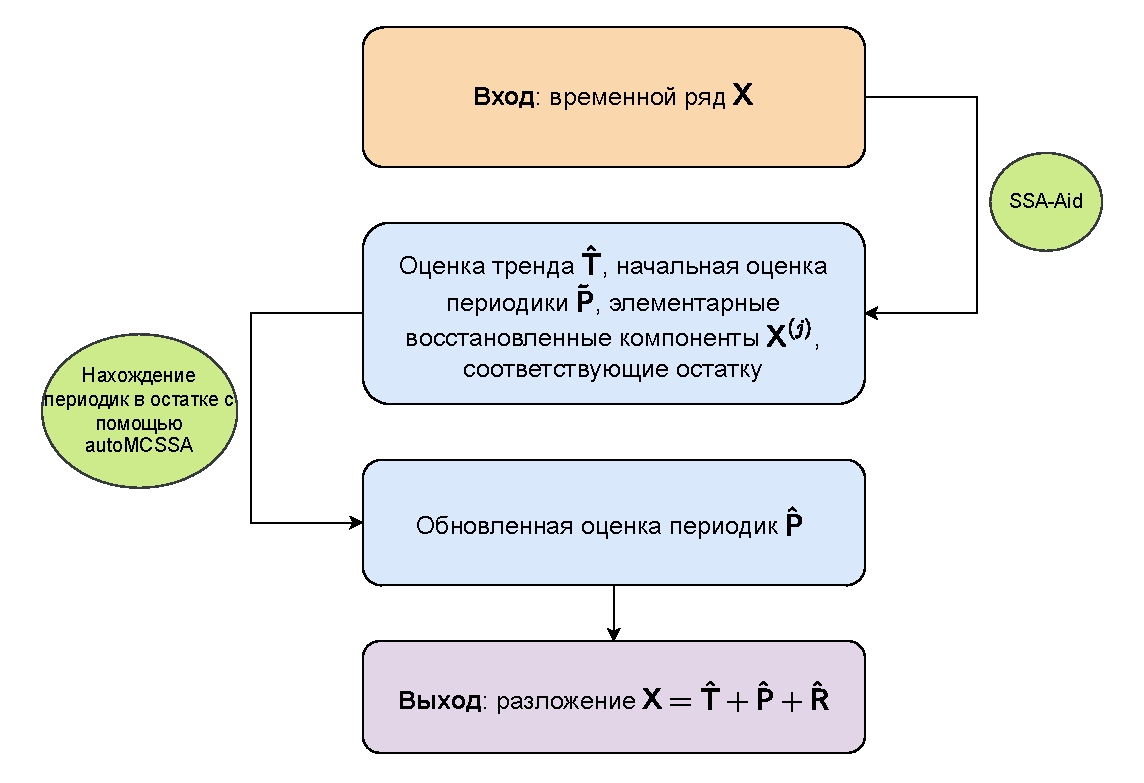
\includegraphics[width=0.9\textwidth]{img/ssa_aidmc_flowchart.pdf}
	\caption{Блок-схема метода SSA-AidMC}
	\label{fig:ssa_aidmc_flowchart}
\end{figure}

\subsection{Выбор параметров метода}

Как можно заметить, алгоритм~\ref{alg:ssa_aid_mc} имеет внушительное количество параметров, однако большинство из имеют в той или иной степени рекомендации к их выбору.

Длину окна $L_\text{SSA}$ для метода SSA следует выбрать исходя из теории SSA: для достижения лучшей (слабой) разделимости компонент длина окна должна быть достаточно большой ($L_\text{SSA}\approx N / 2$); помимо этого, если известно, что в ряде присутствует гармоника, имеет смысл взять длину окна, кратную периоду этой гармоники~\cite{Golyandina2001}.

Длину окна $L_\text{MC-SSA}$ для метода MC-SSA следует выбирать так, чтобы мощность критерия была наибольшей. Как было показано в разделе~\ref{sect:mcssa_comp}, если предполагается, что в ряде присутствуют периодики с амплитудной модуляцией, $L_\text{MC-SSA}$ не должна быть слишком большой, поскольку чем больше длина окна, тем сильнее растекается частота, соответствующая сигналу и тем меньше мощность критерия. С другой стороны, длина окна должна давать достаточную дискретизацию частот спектра (напомним, что длине окна $L$ соответствуют частоты $k/(2L)$), чтобы адекватно идентифицировать значимую частоту. Как и в случае $L_\text{SSA}$, если известен предполагаемый период сигнала, стоит выбирать длину окна, кратную этому периоду: это повышает мощность критерия против данной альтернативы.   

Поскольку для реальных рядов неизвестно значение ранга сигнала, оценку ранга сигнала $r$ следует брать с запасом. Поскольку метод SSA-AidMC базируется на методе SSA-Aid (алгоритм ~\ref{alg:auto_ssa}), который по построению устойчив к завышению ранга сигнала~\cite{Dudnik2025}, для него это также не является проблемой.

Порог низких частот $\omega_0$ задается исходя из того, какие частоты считаются трендовыми. В случае, когда известны частоты тренда и периодические частоты, следует выбрать значение $\omega_0$, лежащее между наибольшей частотой тренда и наименьшей периодической частотой, например, $\omega_0=1/24$ для месячных временных рядов с сезонностью. Порог низких частот $T_\text{low}$ рекомендуется брать равным $0.5$~\cite{autoSSA}.

Как было показано в разделе~\ref{sect:delta_choice_numerical_research}, оптимальные значения для порога $T_0$ лежат в диапазоне $[0.4, 0.5]$, поэтому, как и в случае с порогом $T_\text{low}$, будем брать $T_0=0.5$.

Верхняя граница амплитудной модуляции $C_\text{max}$ определяется по виду ряда и, как было показано в разделе~\ref{sect:C_max}, ее можно выбирать с запасом, например, $C_\text{max}=5$.

\subsection{Численное сравнение точности идентификации компонент}\label{sect:ssa_aid_mc_comparison}

Сравним описанные выше методы по точности выделения различных сигналов. Будем сравнивать три метода: autoMCSSA (алгоритм~\ref{alg:autoMCSSA}), SSA-Aid (алгоритм~\ref{alg:auto_ssa}) и SSA-AidMC (алгоритм~\ref{alg:ssa_aid_mc}). Рассматриваемые ряды имеют следующую модель:
\[
	\tX = \tT + \tP + \bm{\xi},
\]
где $N=200$, $\tT=(t_1,\ldots, t_N)$~--- тренд, $\tP=(p_1,\ldots, p_N)$~--- периодика, $\bm\xi$~--- шум. Количество симуляций для оценки MSE~--- 500.

\begin{remark}
	Стоит уточнить, что до этого момента ряды с трендом не рассматривались, поэтому метод autoMCSSA умеет работать только с периодичностью. Однако можно сначала применить алгоритм autoEOSSA~\cite{autoSSA} для выделения тренда, а потом применять autoMCSSA к остатку и с нетрендовыми элементарными компонентами.
\end{remark}

Для всех рассмотренных примеров были выбраны следующие параметры (параметры метода SSA-Aid взяты из работы~\cite{Dudnik2025}):
\begin{enumerate}
	\item Длины окна $L_\text{SSA}=96$ и $L_\text{MC-SSA}=48$;
	\item Оценка ранга сигнала $r=30$.
	\item Уровень значимости $\alpha=0.05$ для autoMCSSA и SSA-AidMC, $\alpha=0.01$ для SSA-Aid;
	\item Порог низких частот $\omega_0=1/24$;
	\item Пороги $T_\text{low}=T_0=0.5$;
	\item Максимально возможная модуляция $C_{\max}=5$.
	\item Пороги для метода регулярности углов $t_0=0.05$, $p_0=0.03$.
\end{enumerate}

\subsubsection{Сигнал доминирует над шумом}

Рассмотрим примеры сигналов, доминирующих над шумом, то есть сигналу соответствует первые $t$ компонент, где $t$~--- ранг сигнала.

Рассмотрим следующие модели шума $\bm\xi$:
\begin{enumerate}
	\item Белый шум с дисперсией $\sigma^2=1$;
	\item Красный шум с параметрами $\phi=0.3$ и $\sigma^2=1$, $\mathsf{D}\bm\xi\approx1.0989$;
	\item Процесс ARFIMA(0, $d$, 0) с параметрами $d=0.2$ и $\sigma^2=1$, $\mathsf{D}\bm\xi\approx1.0987$.
\end{enumerate}

\begin{example}\label{eg:signal1}
	\begin{align*}
		t_n & =0.2 e^{0.025n} + 2\cos\left(\frac{2\pi n}{60}\right),                                            \\
		p_n & =4.12\cos\left(\frac{2\pi n}{4}\right) + 4.12\cos\left(\frac{2\pi n}{3}\right) + 6\cdot (-1)^{n}.
	\end{align*}

	\begin{table}[h!]
        \centering
		\caption{MSE восстановления сигнала, случай белого шума ($\sigma^2=1$), пример~\ref{eg:signal1}}
	\label{tab:mse_signal1_wn}
        \begin{tabular}{c|c|c|c}
			Компонента & Метод & Mean MSE & Median MSE \\
			\hline
			Тренд & autoMCSSA & 0.063704 & 0.056327 \\
			& SSA-Aid & 0.04361  & 0.03652 \\
			& SSA-AidMC & 0.04372  & 0.03652 \\
			\hline
			Периодика & autoMCSSA & 0.15015  & 0.07147 \\
			& SSA-Aid & 0.07180  & 0.06608 \\
			& SSA-AidMC & 0.07818  & 0.07105 \\
			\hline
			Сигнал & autoMCSSA & 0.21350  & 0.13867 \\
			& SSA-Aid & 0.11539  & 0.10880 \\
			& SSA-AidMC & 0.12177  & 0.11197 \\
			\hline
		\end{tabular}
    \end{table}

	\begin{table}[h!]
        \centering
		\caption{MSE восстановления сигнала, случай красного шума ($\phi=0.3$, $\sigma^2=1$), пример~\ref{eg:signal1}}
	\label{tab:mse_signal1_rn}
		\begin{tabular}{c|c|c|c}
			Компонента & Метод & Mean MSE & Median MSE \\
			\hline
			Тренд & autoMCSSA & 0.17572  & 0.15898 \\
			& SSA-Aid & 0.10623  & 0.09286 \\
			& SSA-AidMC & 0.10664  & 0.09316 \\
			\hline
			Периодика & autoMCSSA & 0.20079  & 0.05290 \\
			& SSA-Aid & 0.05377  & 0.04891 \\
			& SSA-AidMC & 0.05874  & 0.05005 \\
			\hline
			Сигнал & autoMCSSA & 0.37495  & 0.22399 \\
			& SSA-Aid & 0.16036  & 0.14576 \\
			& SSA-AidMC & 0.16518  & 0.15285 \\
			\hline
		\end{tabular}
    \end{table}

	\begin{table}[h!]
        \centering
		\caption{MSE восстановления сигнала, случай шума с длинной памятью ($d=0.2$, $\sigma^2=1$), пример~\ref{eg:signal1}}
	\label{tab:mse_signal1_fi}
		 \begin{tabular}{c|c|c|c}
			Компонента & Метод & Mean MSE & Median MSE \\
			\hline
			Тренд & autoMCSSA & 0.25176  & 0.23243 \\
			& SSA-Aid & 0.18660  & 0.17058 \\
			& SSA-AidMC & 0.18745  & 0.17185 \\
			\hline
			Периодика & autoMCSSA & 0.17576  & 0.05760 \\
			& SSA-Aid & 0.05778  & 0.05271 \\
			& SSA-AidMC & 0.06280  & 0.05435 \\
			\hline
			Сигнал & autoMCSSA & 0.42597  & 0.30628 \\
			& SSA-Aid & 0.24401  & 0.22586 \\
			& SSA-AidMC & 0.24961  & 0.22942 \\
			\hline
			\end{tabular}
    \end{table}
\end{example}

\begin{example}\label{eg:signal2}
	\begin{align*}
		t_n & =0.2 e^{0.025n} + 2\cos\left(\frac{2\pi n}{60}\right),                                                           \\
		p_n & =4 e^{-0.01n}\cos\left(\frac{2\pi n}{4}\right) + 4\cos\left(\frac{2\pi n}{3}\right) + 6e^{-0.01n}\cdot (-1)^{n}.
	\end{align*}

	\begin{table}[h!]
        \centering
        \caption{MSE восстановления сигнала, случай белого шума ($\sigma^2=1$), пример~\ref{eg:signal2}}
		\label{tab:mse_signal2_wn}
        \begin{tabular}{c|c|c|c}        
			Компонента & Метод & Mean MSE & Median MSE \\
			\hline
			Тренд & autoMCSSA & 0.063607 & 0.055946 \\
			& SSA-Aid & 0.043717 & 0.036592 \\
			& SSA-AidMC & 0.043721  & 0.036592 \\
			\hline
			Периодика & autoMCSSA & 0.07721  & 0.06963 \\
			& SSA-Aid & 0.07180  & 0.06705 \\
			& SSA-AidMC & 0.07841  & 0.07014 \\
			\hline
			Сигнал & autoMCSSA & 0.14047 & 0.13513 \\
			& SSA-Aid & 0.11540   & 0.10871 \\
			& SSA-AidMC & 0.12201  & 0.11429 \\
			\hline
        \end{tabular}
    \end{table}

	\begin{table}[h!]
        \centering
        \caption{MSE восстановления сигнала, случай красного шума ($\phi=0.3$, $\sigma^2=1$), пример~\ref{eg:signal2}}
		\label{tab:mse_signal2_rn}
		\begin{tabular}{c|c|c|c}
			Компонента & Метод & Mean MSE & Median MSE \\
			\hline
			Тренд & autoMCSSA & 0.17581  & 0.15984 \\
			& SSA-Aid & 0.10619  & 0.09303 \\
			& SSA-AidMC & 0.10656  & 0.09329 \\
			\hline
			Периодика & autoMCSSA & 0.05808  & 0.05206 \\
			& SSA-Aid & 0.05448  & 0.05106 \\
			& SSA-AidMC & 0.05847  & 0.05204 \\
			\hline
			Сигнал & autoMCSSA & 0.23168  & 0.21785 \\
			& SSA-Aid & 0.16035  & 0.14724 \\
			& SSA-AidMC & 0.16477  & 0.15108 \\
			\hline
		\end{tabular}
    \end{table}

	\begin{table}[h!]
        \centering
        \caption{MSE восстановления сигнала, случай шума с длинной памятью ($d=0.2$, $\sigma^2=1$), пример~\ref{eg:signal2}}
		\label{tab:mse_signal2_fi}
		\begin{tabular}{c|c|c|c}
			Компонента & Метод & Mean MSE & Median MSE \\
			\hline
			Тренд & autoMCSSA & 0.25383  & 0.23167 \\
			& SSA-Aid & 0.18653  & 0.17045 \\
			& SSA-AidMC & 0.18759  & 0.17206 \\
			\hline
			Периодика & autoMCSSA & 0.06260  & 0.05612 \\
			& SSA-Aid & 0.05762  & 0.05485 \\
			& SSA-AidMC & 0.06317  & 0.05614 \\
			\hline
			Сигнал & autoMCSSA & 0.31368  & 0.29704 \\
			& SSA-Aid & 0.24370  & 0.22807 \\
			& SSA-AidMC & 0.25004  & 0.23343 \\
			\hline
		\end{tabular}
    \end{table}
\end{example}

В таблицах~\ref{tab:mse_signal1_wn},~\ref{tab:mse_signal1_rn},~\ref{tab:mse_signal1_fi},~\ref{tab:mse_signal2_wn},~\ref{tab:mse_signal2_rn} и~\ref{tab:mse_signal2_fi} представлены среднее и медианное MSE восстановления тренда, периодики и всего сигнала для кажой расссматриваемой модели шума $\bm\xi$. Из этих таблиц можно увидеть следующее:
\begin{enumerate}
	\item Хуже всего справился autoMCSSA как в оценке тренда, так и в оценке периодики. Б\'{о}льшая ошибка в оценке тренда связана с завышенным рангом сигнала ($r=30$), а оценке периодики~--- с отсутствием сильной разделимости гармоник с периодами $4$ и $3$;
	\item Для SSA-AidMC и SSA-Aid среднее и медианное MSE не сильно отличаются, что может говорить об устойчивости алгоритмов. С другой стороны, у autoMCSSA среднее MSE заметно больше медианного.
	\item SSA-Aid и SSA-AidMC практически не отличаются по точности выделения тренда: разница средних в парном t-критерии значима только в случае модели шума ARFIMA(0, $d$, 0).  
	\item В точности выделения периодики SSA-Aid и SSA-AidMC, хотя и не слишком сильно, но отличаются: разница в средних значима в каждой рассматриваемой модели шума.
\end{enumerate}

\subsubsection{Шум доминирует над некоторыми компонентами сигнала}

Рассмотрим примеры сигналов, некоторые компоненты которых не доминируют над шумом.

Рассмотрим следующие модели шума $\bm\xi$:
\begin{enumerate}
	\item Красный шум с параметрами $\phi=0.7$ и $\sigma^2=1$, $\mathsf{D}\bm\xi\approx1.9608$;
	\item Процесс ARFIMA(0, $d$, 0) с параметрами $d=0.4$ и $\sigma^2=1$, $\mathsf{D}\bm\xi\approx2.0701$.
\end{enumerate}

\begin{example}\label{eg:signal3}
	\begin{align*}
		t_n & = 0.05n,\\
		p_n & = \cos\left(\frac{2 \pi n}{8}\right) + 0.8\cos\left(\frac{2 \pi n}{4}\right) + 0.2\cdot (-1)^n.
	\end{align*}

	\begin{table}[h!]
		\centering
		\caption{MSE восстановления сигнала, случай красного шума ($\phi=0.7$, $\sigma^2=1$), пример~\ref{eg:signal3}}
		\label{tab:mse_signal3_rn}
		\begin{tabular}{c|c|c|c}
			Компонента & Метод & Mean MSE & Median MSE \\
			\hline
			Тренд & autoMCSSA & 0.93705  & 0.88430 \\
			& SSA-Aid & 0.75702  & 0.73264 \\
			& SSA-AidMC & 0.67193  & 0.64756 \\
			\hline
			Периодика & autoMCSSA & 0.11670  & 0.09334 \\
			& SSA-Aid & 0.36983  & 0.30517 \\
			& SSA-AidMC & 0.09988  & 0.08944 \\
			\hline
			Сигнал & autoMCSSA & 1.03212 & 0.97698 \\
			& SSA-Aid & 1.10023  & 1.04891 \\
			& SSA-AidMC & 0.76530  & 0.74120 \\
		\end{tabular}
	\end{table}

	\begin{table}[h!]
		\centering
		\caption{MSE восстановления сигнала, случай шума с длинной памятью ($d=0.4$, $\sigma^2=1$), пример~\ref{eg:signal3}}
		\label{tab:mse_signal3_fi}
		\begin{tabular}{c|c|c|c}
			Компонента & Метод & Mean MSE & Median MSE \\
			\hline
			Тренд & autoMCSSA & 1.30061  & 0.95479 \\
			& SSA-Aid & 1.20080  & 0.85764 \\
			& SSA-AidMC & 1.19324  & 0.85769 \\
			\hline
			Периодика & autoMCSSA & 0.08640  & 0.07802 \\
			& SSA-Aid & 0.11507  & 0.09260 \\
			& SSA-AidMC & 0.08629  & 0.07985 \\
			\hline
			Сигнал & autoMCSSA & 1.37545  & 1.05840 \\
			& SSA-Aid & 1.31128  & 0.97677 \\
			& SSA-AidMC & 1.27636  & 0.94729 \\
		\end{tabular}
	\end{table}
\end{example}

\begin{example}\label{eg:signal4}
	\begin{align*}
		t_n & = 0.05n,\\
		p_n & = 0.075 e^{0.02n}\cos\left(\frac{2 \pi n}{8}\right) + 1.5e^{-0.01n}\cos\left(\frac{2 \pi n}{4}\right) + e^{-0.01n}\cdot (-1)^n.
	\end{align*}

	\begin{table}[h!]
		\centering
		\caption{MSE восстановления сигнала, случай красного шума ($\phi=0.7$, $\sigma^2=1$), пример~\ref{eg:signal4}}
		\label{tab:mse_signal4_rn}
		\begin{tabular}{c|c|c|c}
			Компонента & Метод & Mean MSE & Median MSE \\
			\hline
			Тренд & autoMCSSA & 0.94400  & 0.88290 \\
			& SSA-Aid & 0.69651  & 0.67877 \\
			& SSA-AidMC & 0.67324  & 0.65120 \\
			\hline
			Периодика & autoMCSSA & 0.14870  & 0.09408 \\
			& SSA-Aid & 0.42177  & 0.32153 \\
			& SSA-AidMC & 0.11317  & 0.09408 \\
			\hline
			Сигнал & autoMCSSA & 1.06679  & 0.97830 \\
			& SSA-Aid & 1.08578  & 1.02239 \\
			& SSA-AidMC & 0.77277  & 0.74446 \\
		\end{tabular}
	\end{table}

	\begin{table}[h!]
		\centering
		\caption{MSE восстановления сигнала, случай шума с длинной памятью ($d=0.4$, $\sigma^2=1$), пример~\ref{eg:signal4}}
		\label{tab:mse_signal4_fi}
		\begin{tabular}{c|c|c|c}
			Компонента & Метод & Mean MSE & Median MSE \\
			\hline
			Тренд & autoMCSSA & 1.32725  & 0.96783 \\
			& SSA-Aid & 1.18787  & 0.86008 \\
			& SSA-AidMC & 1.19253  & 0.87273 \\
			\hline
			Периодика & autoMCSSA & 0.08081  & 0.06413 \\
			& SSA-Aid & 0.13258  & 0.06676 \\
			& SSA-AidMC & 0.07699  & 0.06468 \\
			\hline
			Сигнал & autoMCSSA & 1.39344  & 1.04542 \\
			& SSA-Aid & 1.31456  & 0.96974 \\
			& SSA-AidMC & 1.26487  & 0.93489 \\
		\end{tabular}
	\end{table}
\end{example}

В таблицах~\ref{tab:mse_signal3_rn},~\ref{tab:mse_signal3_fi},~\ref{tab:mse_signal4_rn} и~\ref{tab:mse_signal4_fi} представлены среднее и медианное MSE восстановления тренда, периодики и всего сигнала для каждой рассматриваемой модели шума $\bm\xi$. Из этих таблиц можно сделать следующие выводы:
\begin{enumerate}
	\item SSA-AidMC является безоговорочным лидером, имеющим наименьшие ошибки восстановления сигнала;
	\item autoMCSSA все еще имеет наибольшую ошибку при выделении тренда. Причина та же: завышенный ранг сигнала $r$. Однако в оценке периодик метод немного уступает SSA-AidMC: разница в средних значима только в случае модели красного шума;
	\item SSA-Aid оказался наихудшим в оценке периодик, особенно это заметно в модели красного шума.
\end{enumerate} 

\begin{remark}
	Поскольку метод SSA-Aid при отвержении гипотезы $H_0:\tS=0$ выделяет компоненты с наибольшей суммой квадратов, в случае недоминирующего сигнала метод показывает плохие результаты, вне зависимости от значения порогов $t_0$ и $p_0$.
\end{remark}

\conclusion

В ходе данной работы был реализован метод Monte Carlo SSA, когда в качестве модели шума рассматривается процесс с длинной памятью, а также его численное сравнение с Monte Carlo SSA с моделью красного шума, обладающей такой же дисперсией. Было получено, что если в качестве альтернативы рассмотреть сигнал с некоторой частотой, б\'{о}льшую мощность против этой альтернативы дает та модель шума, спектральная плотность которой в этой частоте наименьшая.

Помимо этого, было проведено численное сравнение различных методов оценки параметров модели ARFIMA$(p, d, q)$. Для этого были реализованы методы максимального правдоподобия и Whittle, а также были взяты функции из пакетов языка программирования \textsf{R}. Получено, что при известном среднем метод максимального правдоподобия является наилучшим методом, дающим наименьшую среднеквадратичную ошибку и смещение параметров. Если же среднее неизвестно, наиболее предпочтительным методом является Whittle. Отметим, что реализованный метод максимального правдоподобия оказался лучше, чем в пакете \textsf{arfima}, а качественной реализации метода Whittle на момент написания работы обнаружено не было.

Особое внимание было уделено сравнению способов задания проекционных векторов в модели красного шума: порожденных исходным рядом и представляющих собой косинусы с равноотстоящими частотами. Численные эксперименты показали, что проекция на косинусы дает более мощный критерий в большинстве случаев, особенно при наличии экспоненциальной модуляции сигнала.

Основываясь на полученных результатах сравнения способов задания проекционных векторов, был разработан метод autoMCSSA, позволяющий автоматически идентифицировать значимые компоненты. Проведенные эксперименты подтвердили, что autoMCSSA способен корректно идентифицировать значимые компоненты, которые не обязательно доминируют по вкладу. Также были сформулированы рекомендации по выбору параметров метода.

В связи с неустойчивостью autoMCSSA в случае неразделимости элементарных восстановленных компонент сигнала между собой, была предложена его модификация, которая использует autoMCSSA и метод SSA-Aid, предложенный в~\cite{Dudnik2025}. Было проведено численное сравнение этих трех методов на разных примерах. Получено, что предложенная модификация стала точнее выделять сигнал. При этом она сохранила возможность идентифицировать значимые компоненты, которые не обязательно доминируют по вкладу, в отличие от метода SSA-Aid, который корректно работает только в случае, когда сигналу соответствуют первые $r$ компонент разложения.

\bibliographystyle{ugost2008}
\bibliography{report}

\appendix

\chapter{Графики}

\section{Сравнение \textsf{arfima\_mle} и \textsf{arfima}}\label{sect:mle_comparison}

На рис.~\ref{fig:mle_comparison_phi1},~\ref{fig:mle_comparison_phi5} и~\ref{fig:mle_comparison_phi9} представлены среднеквадратичное отклонение, смещение и дисперсия оценок параметров $\phi$ и $d$ модели $\textrm{ARFIMA}(1, d, 0)$. По ним, видно, что при $\phi=0.1$ на рис.~\ref{fig:mle_comparison_phi1} оценки функцией \textsf{arfima} имеют скачок в $d=0.4$, что может говорить о некоторой вычислительной неустойчивости функции для больших $d$. Функция \textsf{arfima\_mle} не только не имеет подобной проблемы, но и дает более точные оценки, например, при $\phi=0.5$ на рис.~\ref{fig:mle_comparison_phi5}.

\begin{figure}[h]
	\centering
	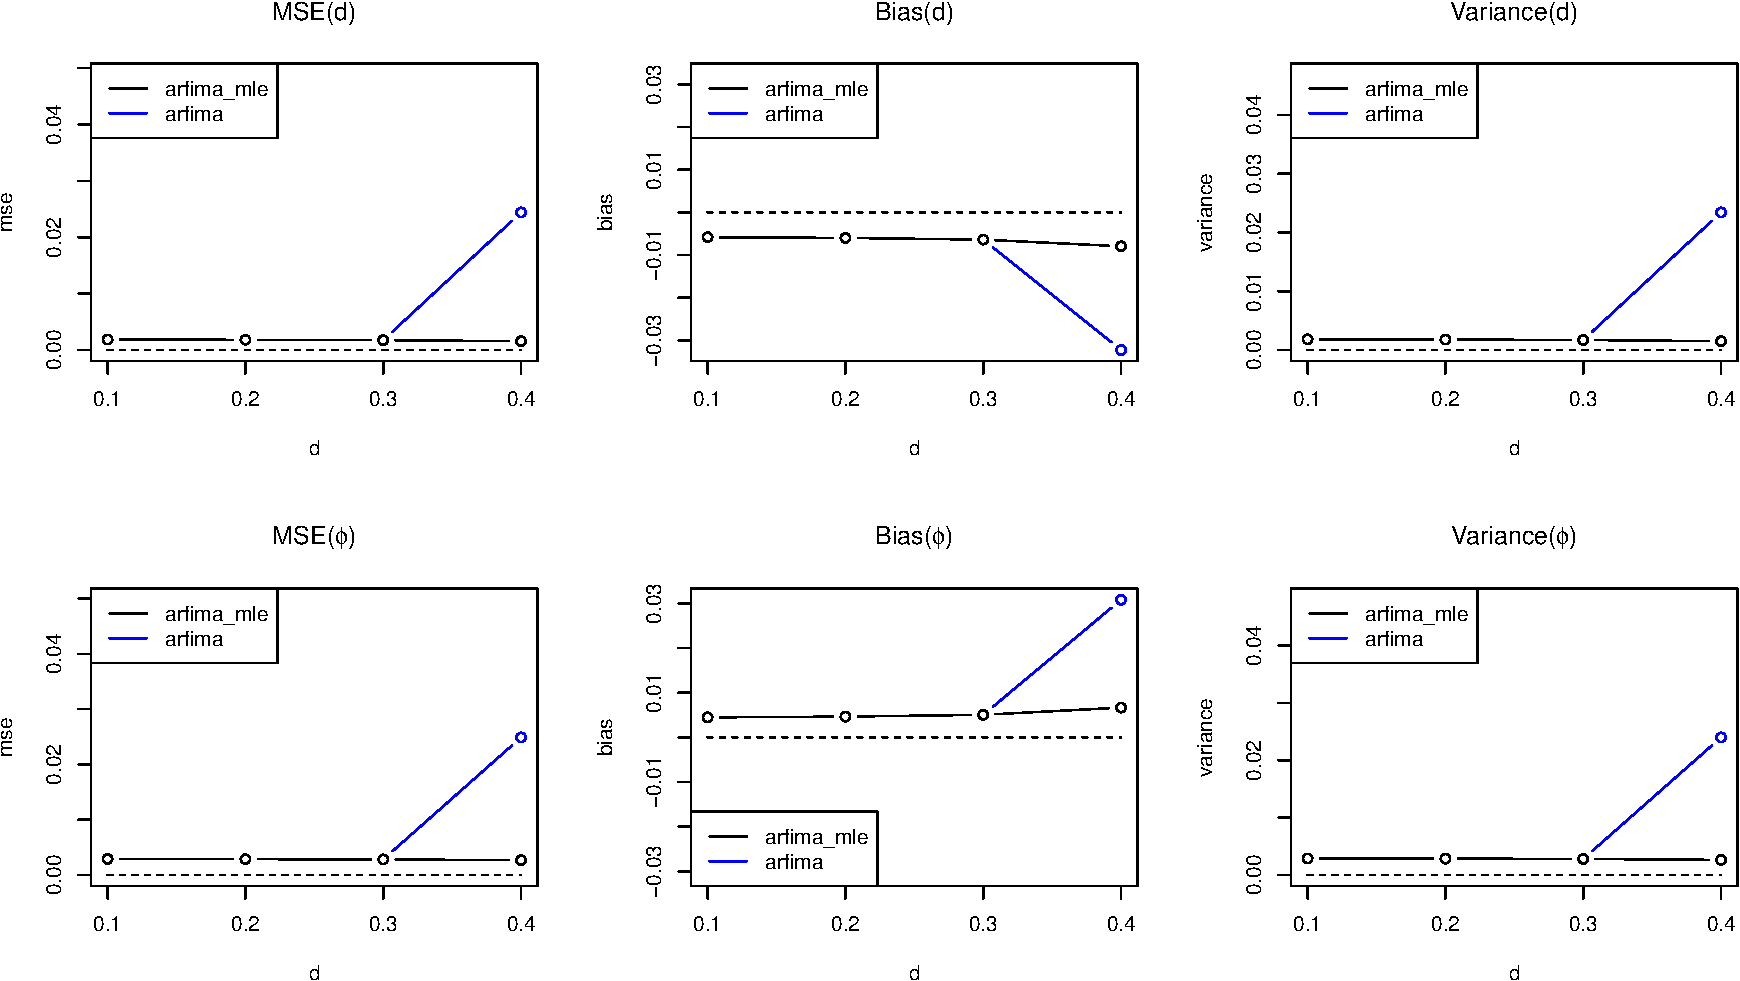
\includegraphics[width=\textwidth]{img/arfi_est_phi1.pdf}
	\caption{Сравнение \textsf{arfima\_mle} и \textsf{arfima} при $\phi=0.1$ ($n=1000$, $500$ повторений)}
	\label{fig:mle_comparison_phi1}
\end{figure}

\begin{figure}[h]
	\centering
	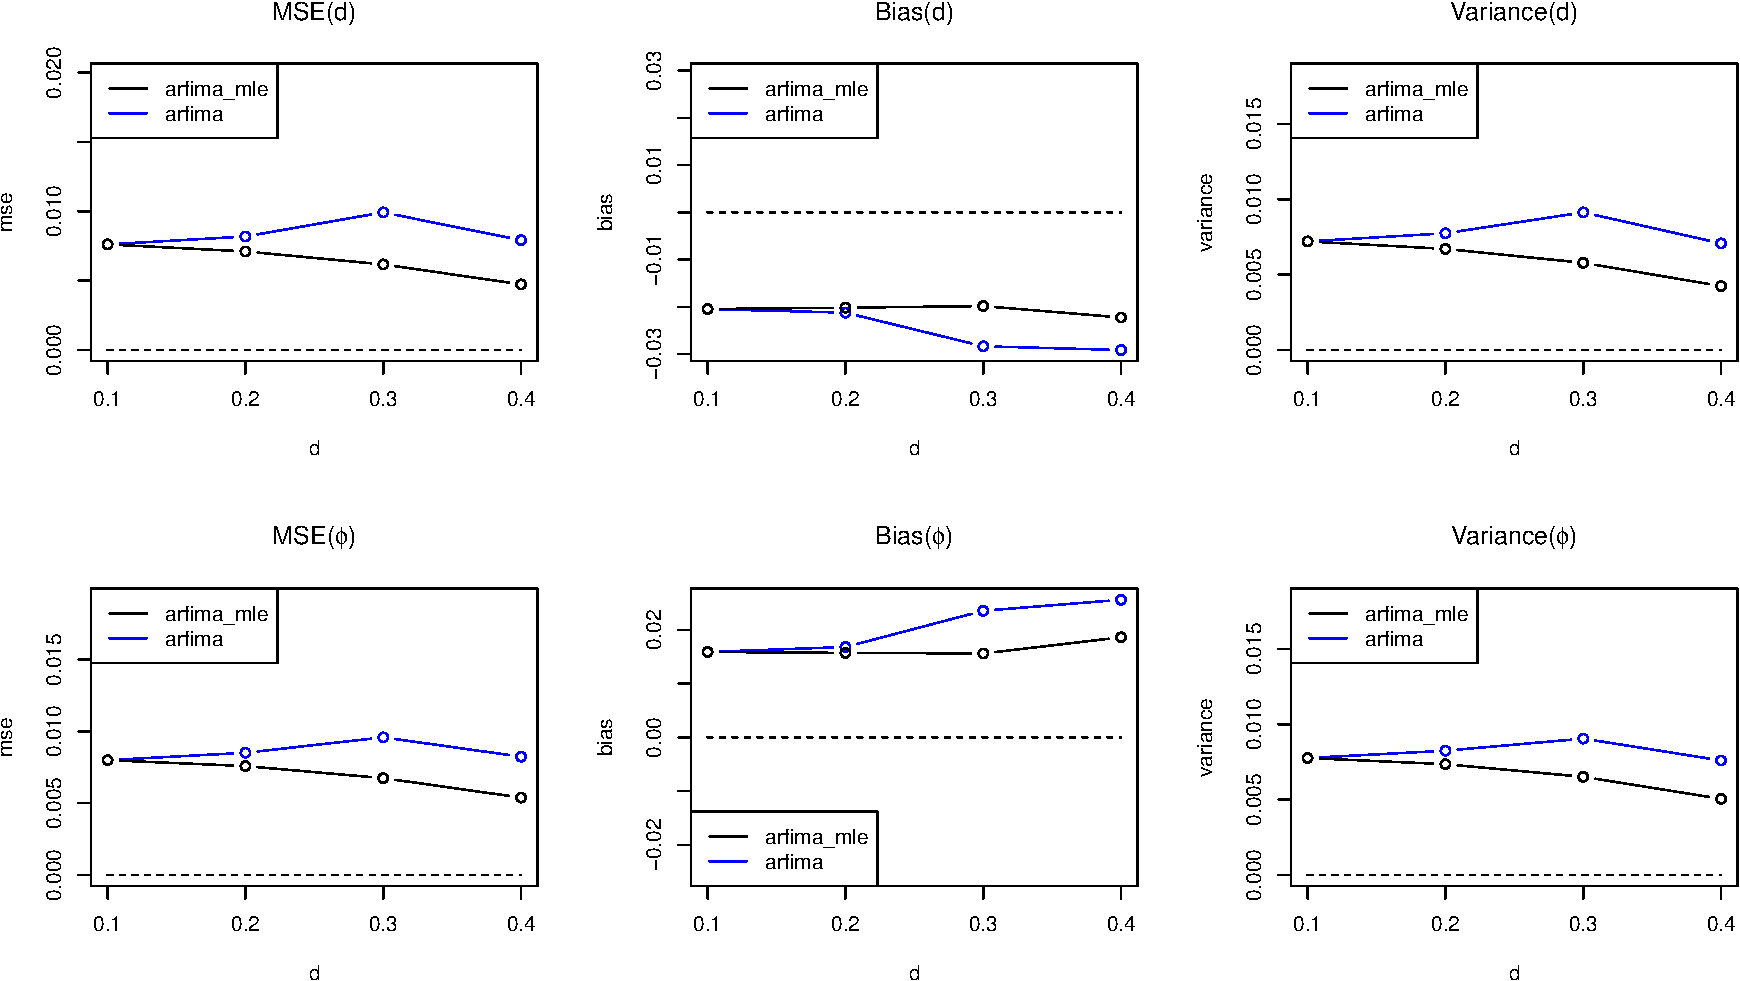
\includegraphics[width=\textwidth]{img/arfi_est_phi5.pdf}
	\caption{Сравнение \textsf{arfima\_mle} и \textsf{arfima} при $\phi=0.5$ ($n=1000$, $500$ повторений)}
	\label{fig:mle_comparison_phi5}
\end{figure}

\begin{figure}[h]
	\centering
	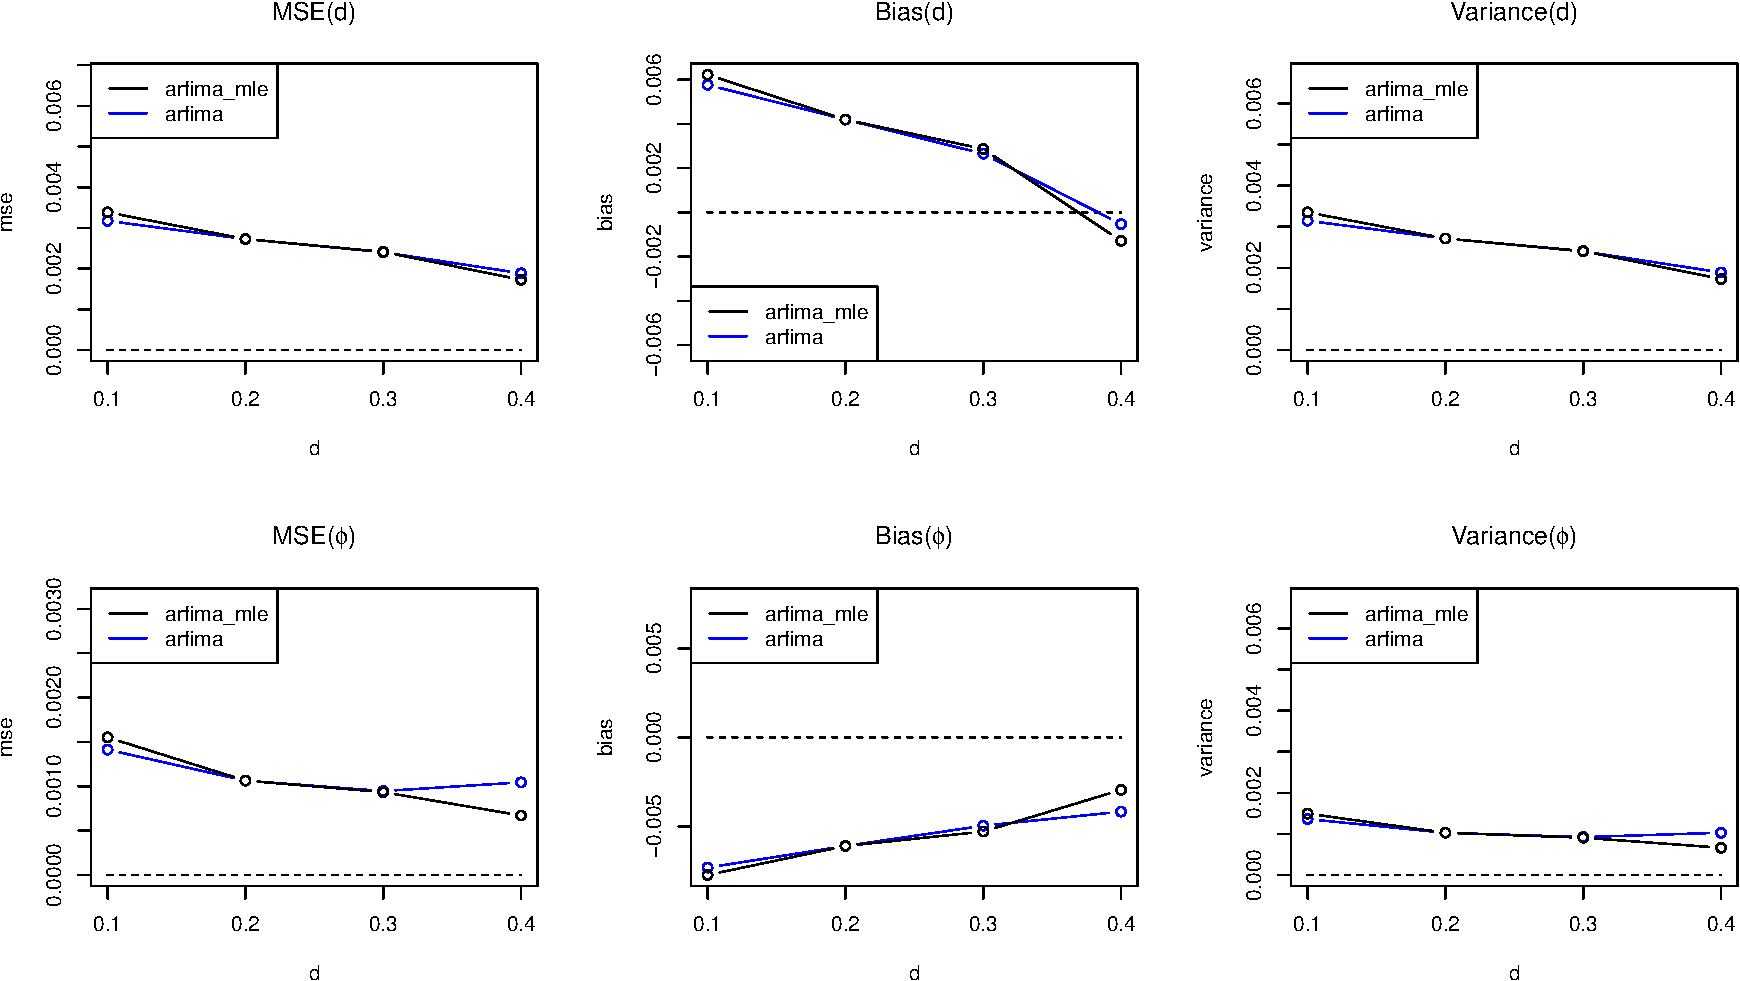
\includegraphics[width=\textwidth]{img/arfi_est_phi9.pdf}
	\caption{Сравнение \textsf{arfima\_mle} и \textsf{arfima} при $\phi=0.9$ ($n=1000$, $500$ повторений)}
	\label{fig:mle_comparison_phi9}
\end{figure}

\chapter{Подходы к выделению сигнала в методе autoMCSSA}\label{chpt:signal_extraction_approaches}

При описании алгоритма autoMCSSA (алгоритм~\ref{alg:autoMCSSA}) для выделения сигнала $\tS$ использовалось разложение базового варианта SSA. Можно обобщить этот подход на SSA с проекцией, зафиксировав подходящий базис.

\section{SSA с проекцией}\label{sect:ssa_with_proj}

Базовый вариант SSA использует адаптивный базис для оценки подпространства сигнала, но существует возможность зафиксировать некоторые компоненты разложения. Пусть $\bfD\in\R^{L\times m}$~--- матрица, проекцию на столбцы которой мы хотим зафиксировать в разложении $\mathbf{X}$. Тогда SSA с проекцией отличается от базового алгоритма только шагом разложения:
\begin{enumerate}
	\item В случае, если столбцы матрицы $\mathbf{D}$ не ортонормированны, $\mathbf{D}$ приводится к нужному виду путем ортогонализации Грамма-Шмидта.
	\item Вычисляется матрица $\bfC=\bfD\bfD^\rmT\bfX$.
	\item Вычисляется матрица $\bfX^\star=\bfX-\bfC$.
	\item Матрица $\bfX^\star$ раскладывается в сумму матриц ранга $1$.
\end{enumerate}

\begin{remark}
	Таким же образом можно определить SSA с проекцией на строки некоторой матрицы $\bfM\in\R^{l\times K}$.
\end{remark}

\section{Рассматриваемые подходы}

Будем считать, что сигнал представляет из себя экспоненциально-модулированную гармонику~\eqref{eq:em_harmonic} с $\omega\in(0, 0.5)$. Пусть $\hat\omega$~--- оценка $\omega$. Обозначим
\[
	D_1=\begin{pmatrix}
		\cos(2\pi\hat\omega 1) \\
		\ldots                 \\
		\cos(2\pi\hat\omega L_\text{SSA})
	\end{pmatrix}, \,
	D_2=\begin{pmatrix}
		\sin(2\pi\hat\omega 1) \\
		\ldots                 \\
		\sin(2\pi\hat\omega L_\text{SSA})
	\end{pmatrix}\in \R^{L_\text{SSA}}.
\]
Рассмотрим следующие варианты выделения сигнала $\mathsf{S}$ по частоте $\hat \omega$:
\begin{enumerate}
	\item <<adaptive>>: получить разложение исходного ряда на элементарные восстановленные компоненты с помощью SSA и применить алгоритм~\ref{alg:auto_periodic};
	\item  <<semi-adaptive>>: применить SSA с проекцией с $\mathbf{D}=D_1\in \R^{L_\text{SSA}\times 1}$, получить разложение исходного ряда на элементарные восстановленные компоненты и выбрать, помимо компоненты, соответствующей вектору $D_1$, первую компоненту разложения, у которой мера $T$~\eqref{eq:freq_measure} на интервале $[\hat\omega-\delta, \hat\omega+\delta]$, $\delta\geqslant0$, больше некоторого порога $T_0\in[0, 1]$;
	\item <<fixed>>: применить SSA с проекцией с $\mathbf{D}=[D_1:D_2]\in\R^{L_\text{SSA}\times 2}$, получить разложение исходного ряда на элементарные восстановленные компоненты и выбрать компоненты, соответствующие векторам $D_1$, $D_2$.
\end{enumerate}
Заметим, что вариант <<adaptive>> соответствует методу, который используется в методе autoMCSSA (алгоритм~\ref{alg:autoMCSSA}).

\subsection{Численное сравнение подходов}

Проведем численный эксперимент с целью понять, какой из предложенных способов восстановления сигнала наиболее точен. Пусть $N=99$, процесс $\bm\xi$~--- красный шум с параметрами $\phi=0.7$, $\sigma^2\in\{0.2, 0.4, 0.6, 0.8, 1\}$. Для SSA $L_\text{SSA}=50$, для MC-SSA $L=40$ (выводы устойчивы к выбору длины окна). В вариантах <<adaptive>> и <<semi-adaptive>> $\delta=0.025$ и $T_0=0.5$. Рассмотрим два типа сигнала $\mathsf{S}$, один из которых является частным случаем другого:
\begin{enumerate}
	\item $a=0$, $A=1$~--- гармоника с постоянной амплитудой.
	\item $a=0.05$, $A=0.025$~--- экспоненциально-модулированная гармоника.
\end{enumerate}
Возьмем $\omega=0.115$. Заметим, что при таком выборе частоты сигнала $L \omega$ нецелое, а значит $\omega$ не попадает в решетку $k/(2L)$. Оценивать частоту $\omega$ также как и в autoMCSSA с помощью алгоритма~\ref{alg:signif_freq_est}.

На рис.~\ref{fig:mse1} изображена зависимость MSE восстановления сигнала от дисперсии белого шума $\sigma^2$. По графикам видно, что в случае постоянной амплитуды ($a=0$) выигрывает вариант <<fixed>>, однако в случае непостоянной амплитуды фиксированный базис оказывается наихудшим. Полуадаптивный базис, являясь неким компромиссом между адаптивным и фиксированным базисами, оказывается вторым по точности в случае $a=0$ и сравнимым с адаптивным в рассмотренном случае $a\ne0$. При увеличении $|a|$, начиная с какого-то момента, фиксированная половина базиса ухудшает восстановление сигнала.

Теперь посмотрим, как будут изменяться ошибки при уменьшении/увеличении $\delta$ для фиксированного $L$. На рис.~\ref{fig:mse2} $\delta$ уменьшена, а на рис.~\ref{fig:mse3} увеличена в два раза ($\delta=0.0125$ и $0.05$ соответственно). Из этих графиков видно, что слишком маленькое $\delta$ приводит к ухудшению точности адаптивного и полуадаптивного вариантов в случае $a\ne0$. Связано это с тем, что частота экспоненциально-модулированной гармоники, в отличие от гармоники с постоянной амплитудой, всегда растекается по спектру и чем больше абсолютное значение показателя экспоненты $a$, тем сильнее это растекание. Увеличение $\delta$ в два раза не привело к значительному изменению точности методов, однако, если и дальше увеличивать $\delta$, ошибки, как и в случае слишком маленького $\delta$, опять возрастут.

Исходя из полученных результатов, можно сделать следующие выводы. Во-первых, параметр $\delta$, определяющий длину частотного интервала при отборе компонент, не следует выбирать слишком маленьким, если есть подозрения на амплитудную модуляцию сигнала. Во-вторых, при отсутствии или наличии умеренной амплитудной модуляции следует выбирать полуадаптивный метод, имеющий наименьшее MSE восстановления сигнала среди рассмотренных подходов. Если применить autoMCSSA к рассмотренному в разделе~\ref{sect:autoMCSSA_example} примеру, выделяя сигнал полуадаптивным подходом, то полученная оценка сигнала сравнима с результатом адаптивного подхода.

\begin{figure}[h!]
	\centering
	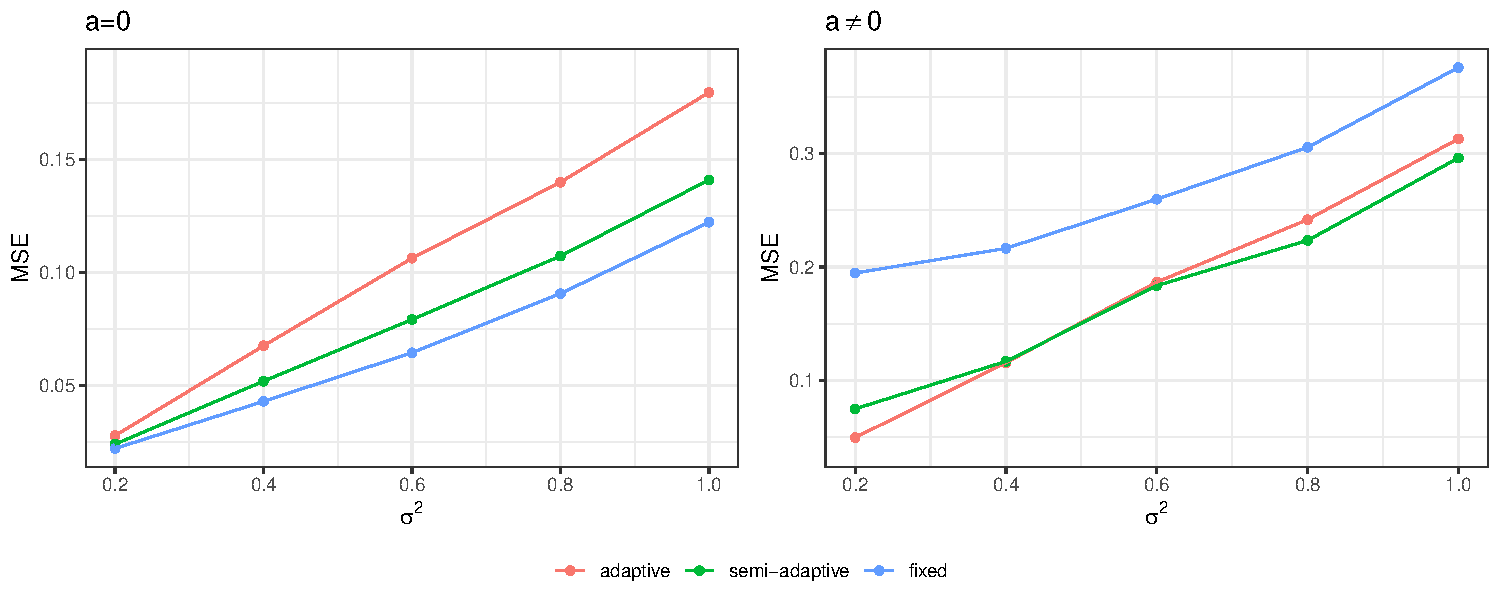
\includegraphics[width=\linewidth]{img/mse.pdf}
	\caption{MSE восстановления сигнала ($\delta=0.025$)}
	\label{fig:mse1}
\end{figure}
\begin{figure}[h!]
	\centering
	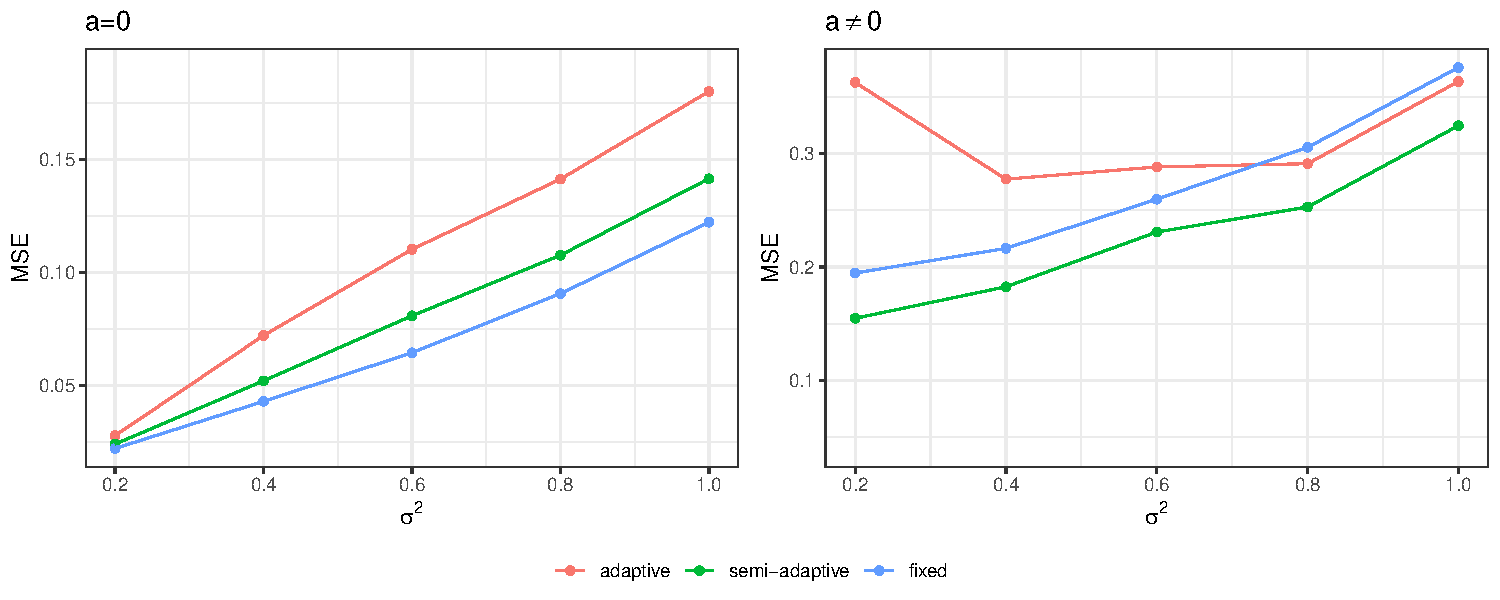
\includegraphics[width=\linewidth]{img/mse_delta_smaller.pdf}
	\caption{MSE восстановления сигнала ($\delta=0.0125$)}
	\label{fig:mse2}
\end{figure}
\begin{figure}[h!]
	\centering
	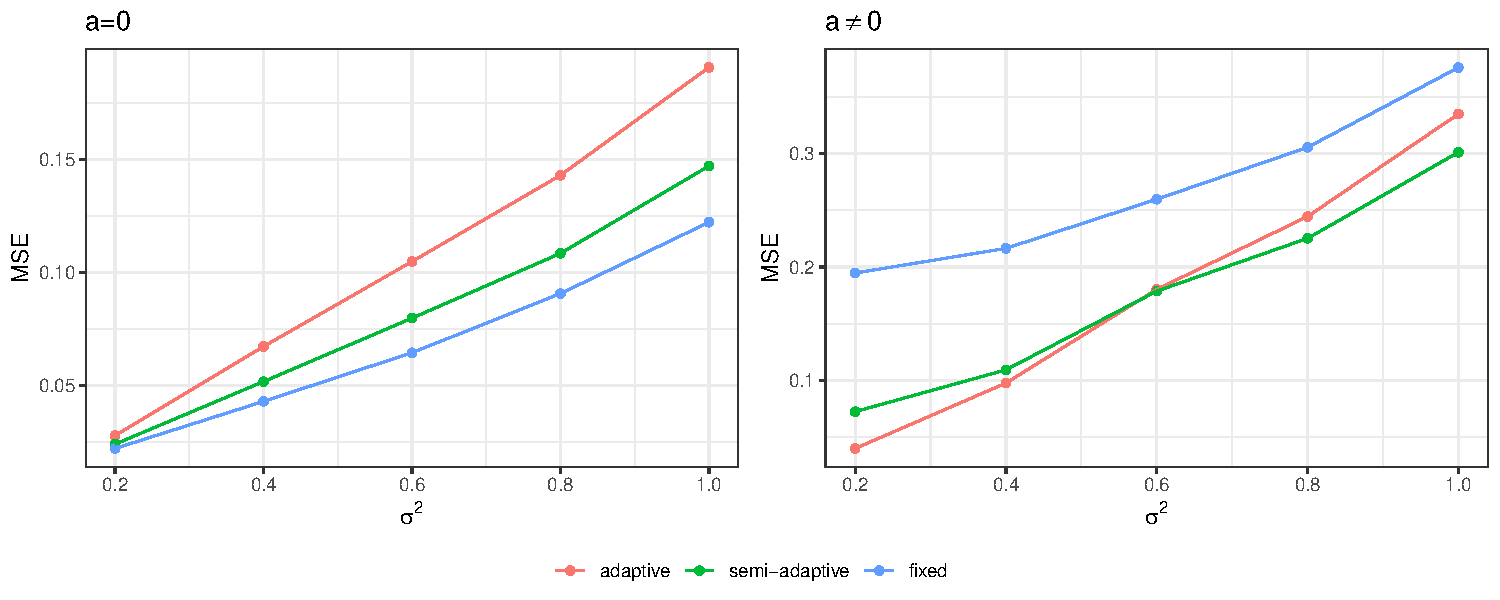
\includegraphics[width=\linewidth]{img/mse_delta_bigger.pdf}
	\caption{MSE восстановления сигнала ($\delta=0.05$)}
	\label{fig:mse3}
\end{figure}

\end{document}
